\section{Evaluation}~\label{sec:evaluation}

\begin{figure*}[!t]
    \centering
    \begin{subfigure}[t]{0.4\textwidth}
        \centering
        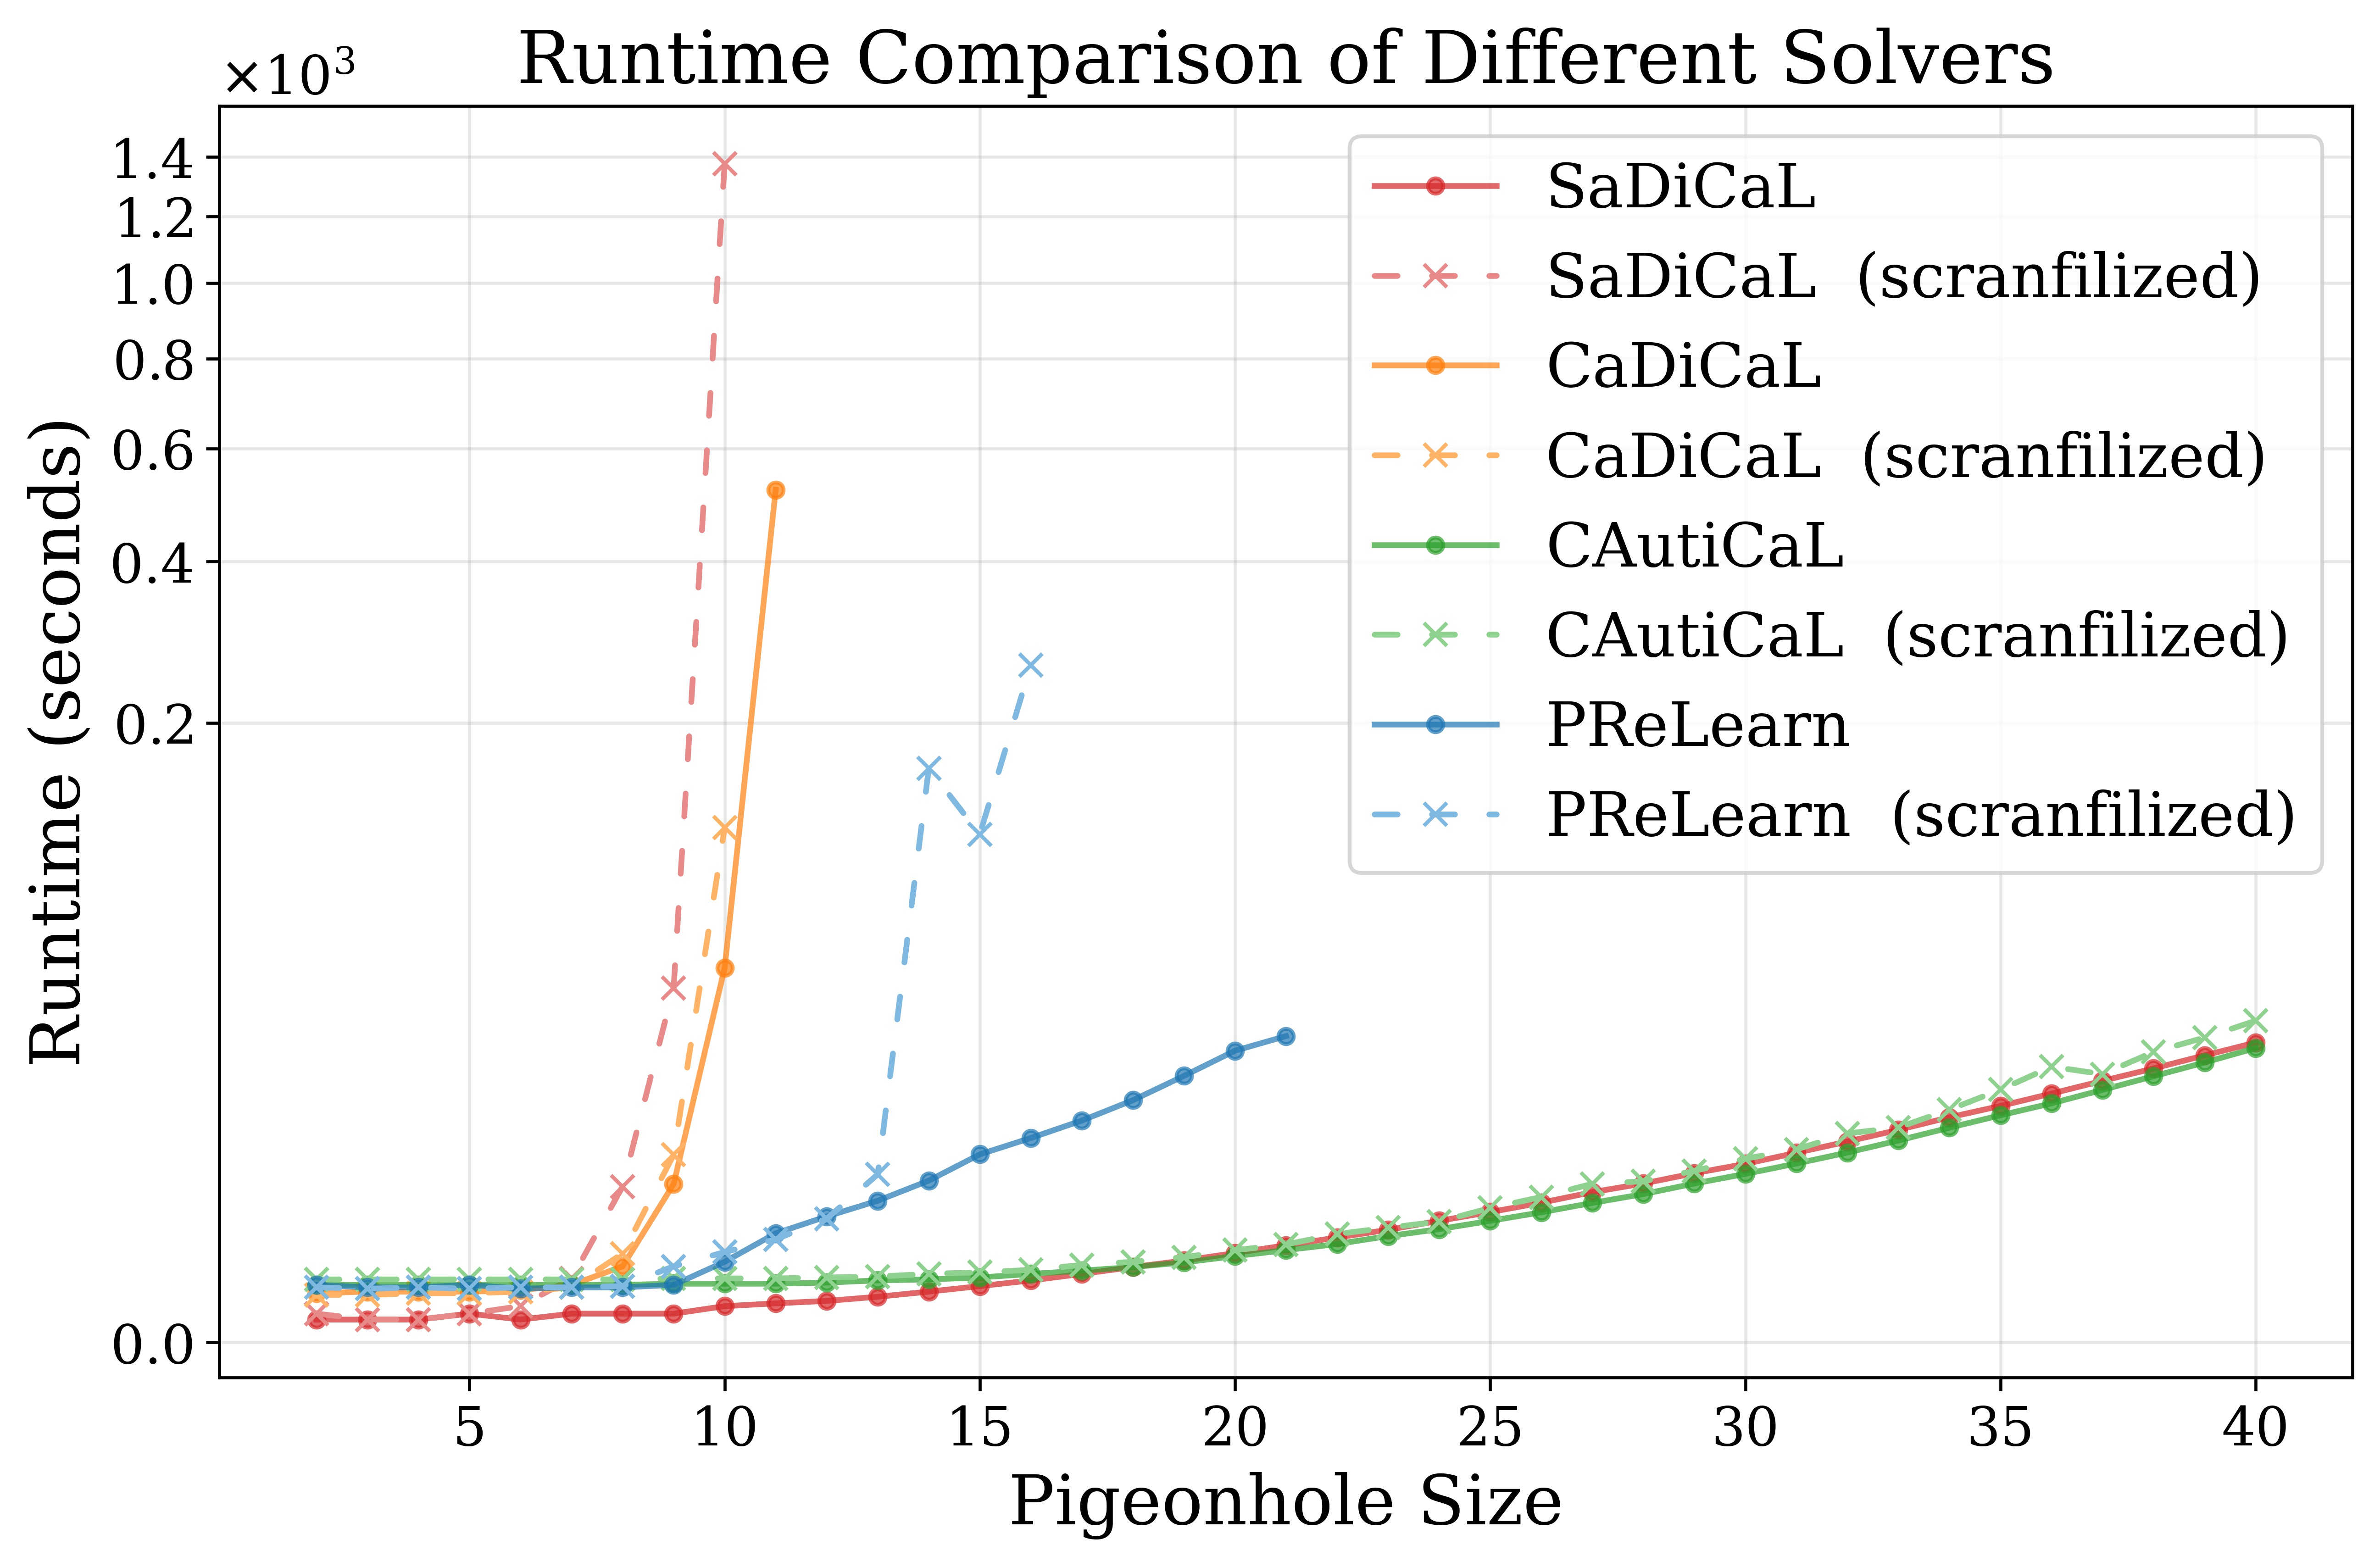
\includegraphics[width=\textwidth]{figs/pigeonhole_runtime_comparison.jpg}
        % \caption{Runtime on Pigeonhole Principle formulas}
        \label{fig:pigeonhole-runtime-comparison}
    \end{subfigure}
    \hspace{0.06\textwidth}
    \begin{subfigure}[t]{0.4\textwidth}
        \centering
        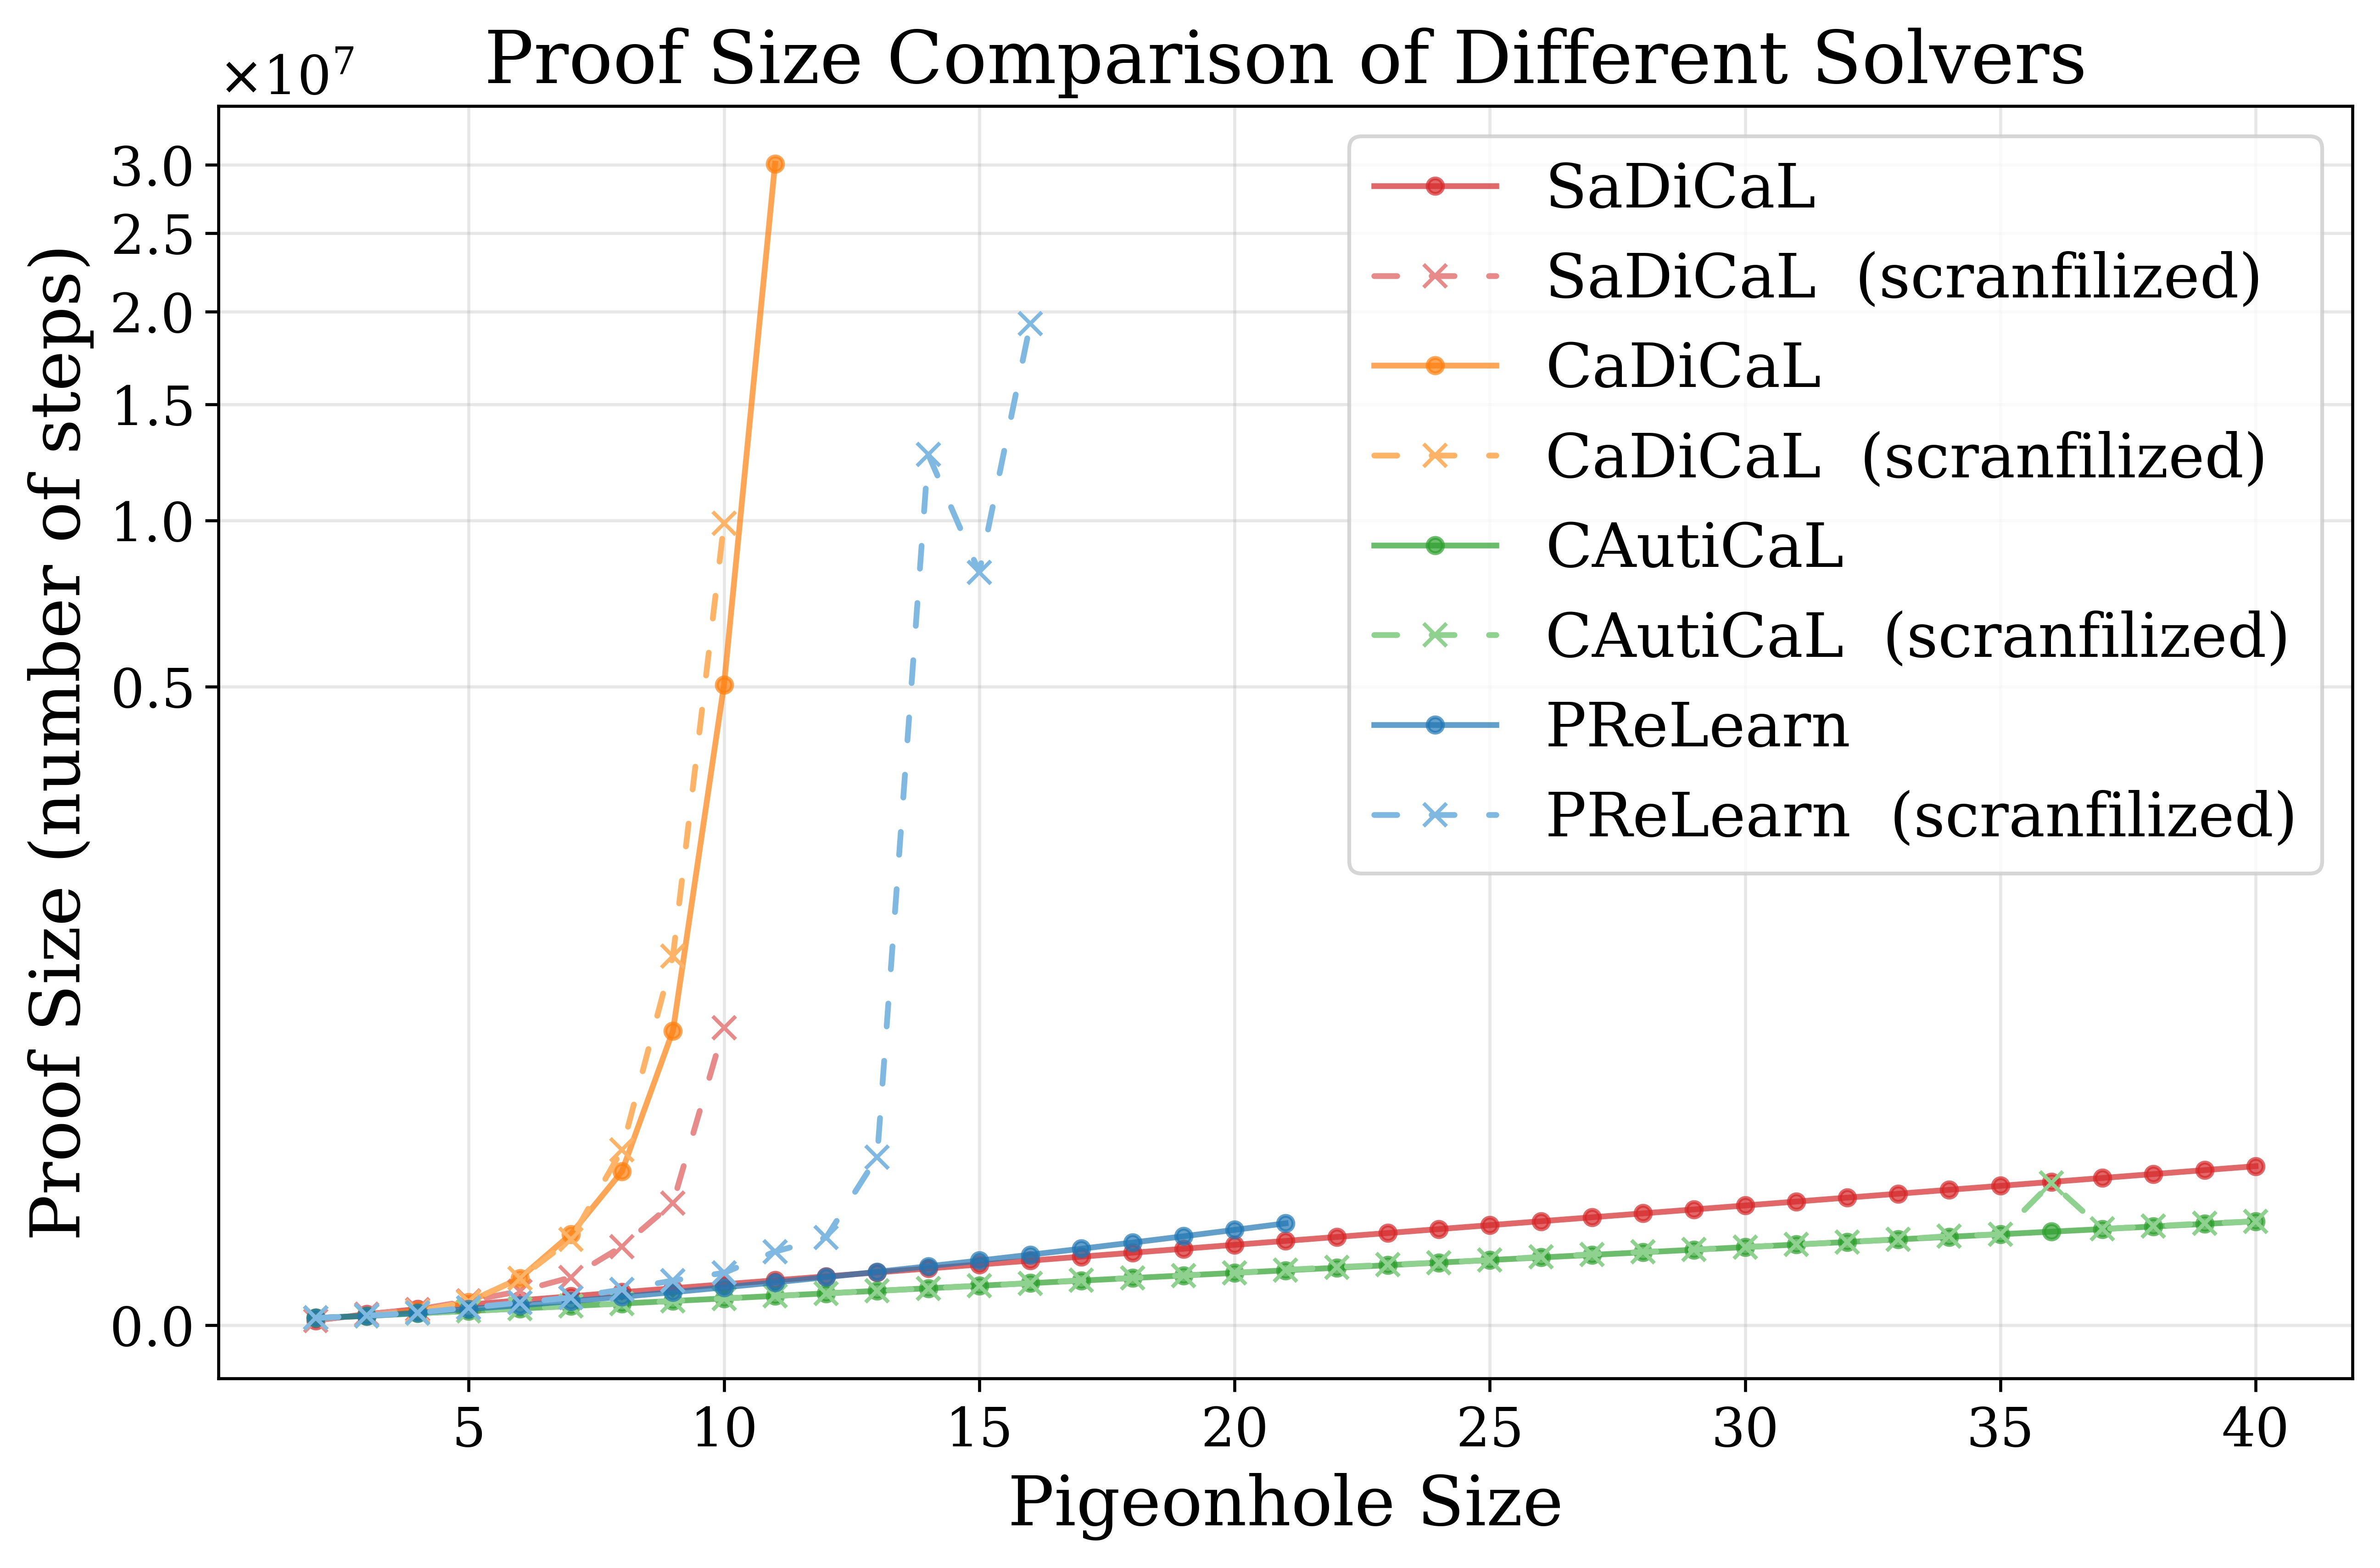
\includegraphics[width=\textwidth]{figs/pigeonhole_proof_size_comparison.jpg}
        % \caption{Proof Size for Pigeonhole Principle formulas}
        \label{fig:pigeonhole-proof-size-comparison}
    \end{subfigure}
    \caption{Comparison of \tool, \cadical, \sadical, and \prelearn on pigeonhole principle benchmarks up to size $40$. The y-axis is on a cube root scale. The performance of a solver on the original benchmark is shown with a solid line. The median of 5 scranfilized queries is shown with a dashed line. If a solver times out on a query in 5000s, it is not shown.}
    \label{fig:pigeonhole-results}
\end{figure*}

In this section, we empirically evaluate our technique against other \pr clause
learning techniques. In doing so, we aim to answer the following research
questions:


\begin{enumerate}[label={RQ\arabic*}]
    \item Can our approach provide a speedup on certain benchmark families?
    \item Is our approach less sensitive to encoding choices compared to other
    \pr learning techniques?
    % \item Can these techniques underperform or outperform SAT solvers on other
    % certain benchmark families?
\end{enumerate}


We compare the two main tools learning \pr clauses: \sadical (based on SDCL) and
\prelearn (a preprocessing technique that calls \sadical). To be consistent with
our approach, we run \prelearn with its default settings for 30 seconds, then
solve the preprocessed formula with \cadical. We also compare to \cadical as a
baseline with no \pr clause learning. We check all proofs of unsatisfiability
from \tool using \texttt{dpr-trim}~\cite{dpr-trim}.

All experiments were performed in the Anvil Supercomputing Center on nodes with
128 cores and 2 GB RAM per core~\cite{anvil}. We ran 64 experiments in parallel
per node with a 5,000 second timeout, the default timeout for the SAT
competition.

In \autoref{subsec:eval-pigeonhole}, we compare all approaches on the pigeonhole
principle, evaluating runtime, proof length, and sensitivity to the encoding of
the formula. In \autoref{subsec:eval-satcomp}, we evaluate the solvers on
benchmarks from the '22, '23, and '24 SAT competition's main
tracks~\cite{satcomp2022,satcomp2023,satcomp2024}. In
\autoref{subsec:eval-discussion}, we highlight certain benchmark families that
benefit from \pr clause learning. In \autoref{sec:heuristics}, we evaluate the 
benefit of different heuristic choices in \tool. Finally, we conclude in 
\autoref{subsec:researchquestions} with a discussion of how performed on RQ1 and 
RQ2.
%We evaluate the different approaches on these families. Finally, we analyze the
% use of specific heuristic choices in \tool by turning heuristics off
% individually and observing their effect (\autoref{subsec:eval-heuristics}). 



\subsection{Pigeonhole results}~\label{subsec:eval-pigeonhole}


Approaches based on SDCL, such as \sadical, are successful for learning $O(n^3)$
proofs for the pigeonhole principle, but are very sensitive to the encoding of
the formula. We compare the solvers on pigeonhole principle from \ph{2} to
\ph{40} and plot these results in \autoref{fig:pigeonhole-results}. As the
expected best-behavior is cubic, we use a cube root scale for the y-axis.

As expected, \cadical grows exponentially, while \sadical and \tool scale
cubicly in both runtime and proof size. Significantly, \tool is able to learn
$3.59$-$3.64\times$ shorter proofs compared to \sadical. 
% on formulas larger than \ph{10} This is because \sadical deletes clauses more
% frequently. , as to not exclude other clauses from being learned. Frequent
% deletion is not necessary in \tool because of its clause shrinking technique. 
\prelearn scales cubicly on small formulas, but for \ph{22} and larger, will not
learn enough useful \pr clauses in the preprocessing step and will timeout after
spending the rest of its time running \cadical.

% As we discuss in \autoref{app:pigeonhole}, \tool learns proofs of size
% $\approx \frac13 n^3$, which is expected to be shorter than known \pr proofs
% for the pigeonhole principle.

Additionally, we evaluate all solvers on scranfilized variations of the
pigeonhole principle. Scranfilization is a technique for generating an
satisfiability-equivalent formula~\cite{scranfilize}. We use the tool
\texttt{scranfilize}~\cite{scranfilize} with the options permuting variables,
permuting clauses, and flipping literals (with probability $0.5$) all turned on.
We run each solver on 5 scranfilized variations for each benchmark and take the
median runtime and proof size. This is shown in \autoref{fig:pigeonhole-results}
with dashed lines.

\sadical and \prelearn exhibit an exponential trend for runtime and proof size
on the scranfilized benchmarks. \sadical will spend all its time in the main
SDCL loop not learning enough useful clauses. \prelearn will learn some useful
\pr clauses in preprocessing, but not enough to sufficiently shrink the search
space for formulas larger than \ph{16}.

On the other hand, \tool almost matches its non-scranfilized performance,
demonstrating that it learns useful \pr clauses regardless of the encoding.

% In conclusion, \tool is able to match \sadical's runtime for the pigeonhole
% principle while shorter proofs by a constant factor. Additionally, \tool is
% insensitive to permuting variables, permuting clauses, and flipping literals
% as it relies on conditional autarkies, a global property of the formula.



\subsection{SAT competition results}~\label{subsec:eval-satcomp}





%   Category                                        0-10k SAT  0-10k UNSAT
% 10k-20M SAT  10k-20M UNSAT  20M+ SAT  20M+ UNSAT  Total Total Formulas 70 132
% 395            416        40          46   1099 Cadical Solved 54           73
% 319            303        35          46    830 Has PR Clauses 57           90
% 224            220         0           3    594 Has Many PR Clauses 36 66 131
% 137         0           0    370 Prelearn Solved 52 90          322 307 35
% 46    852 Prelearn Only 1           17 6              6         0 0     30
% Prelearn Only (on formulas we learn stuff)              1 17            6 5
% 0 0     29 Prelearn Improved 11 42           57 36         1           1
% 148 Prelearn Improved (on formulas we learn stuff) 9           41           51
% 27         0 0    128 Cautical Solved 52 87          317            298
% 32 29    815 Cautical Only 0 18 9              9         0           0     36
% Cautical Only (on formulas we learn stuff)              0           18
% 1 4 0 0     23 Cautical Improved                                      23 48 89
% 59         0           8    227 Cautical Improved (on formulas we learn stuff)
% 7           38            4 7         0           0 56 Blocked Clauses 16 61
% 36             74         0 0    187 Has Many Blocked Clauses 1 42 7 45
% 0           0     95

%   Category                                          0-10k SAT  0-10k UNSAT
% 10k-20M SAT  10k-20M UNSAT        Total Total Formulas 70.000000   132.000000
% 395.000000     416.000000  1013.000000 Cadical Solved 54.000000    73.000000
% 319.000000     303.000000   749.000000 Has PR Clauses 57.000000    90.000000
% 224.000000     220.000000   591.000000 Has Many PR Clauses 36.000000 66.000000
% 131.000000 137.000000   370.000000 Prelearn Solved 52.000000 90.000000
% 322.000000     307.000000   771.000000 Prelearn Only 1.000000 17.000000
% 6.000000       6.000000    30.000000 Prelearn Only (on formulas we learn
% stuff)         1.000000    17.000000     6.000000 5.000000 29.000000 Prelearn
% Only % (on formulas we learn stuff) 0.017544 0.188889 0.026786       0.022727
% 0.255946 Prelearn Improved 11.000000    42.000000 57.000000 36.000000
% 146.000000 Prelearn Improved (on formulas we learn stuff) 9.000000 41.000000
% 51.000000      27.000000 128.000000 Prelearn Improved % (on formulas we learn
% stuff)   0.157895 0.455556     0.227679 0.122727 0.963856 Cautical Solved
% 52.000000 87.000000   317.000000 298.000000 754.000000 Cautical Only 0.000000
% 18.000000     9.000000 9.000000    36.000000 Cautical Only (on formulas we
% learn stuff) 0.000000    18.000000     1.000000 4.000000 23.000000 Cautical
% Only % (on formulas we learn stuff) 0.000000 0.295082 0.027778       0.054054
% 0.376914 Cautical Improved 23.000000 48.000000    89.000000 59.000000
% 219.000000 Cautical Improved (on formulas we learn stuff) 7.000000 38.000000
% 4.000000       7.000000 56.000000 Cautical Improved % (on formulas we learn
% stuff)   0.437500 0.622951     0.111111 0.094595 1.266157 Blocked Clauses
% 16.000000 61.000000    36.000000 74.000000 187.000000 Has Many Blocked Clauses
% 1.000000    42.000000 7.000000 45.000000    95.000000

  % Category                  0-10k SAT  0-10k UNSAT  10k-20M SAT  10k-20M UNSAT
  % 20M+ SAT  20M+ UNSAT  Total
% Total Formulas                   70          132          395            416
% 40          46   1099 -> issue with this total is that certain formula
% statuses are unknown, so not counted here Cadical Solved                   54
% 73          319            303        35          46    830 Has PR Clauses 40
% 73          179            145         0           3    440 Has Many PR
% Clauses              22           51          104             79 0           0
% 256 Prelearn Solved                  52           90 322            307 35 46
% 852 Prelearn Only 1           17            6              6 0 0     30
% Prelearn Improved                11           42 57             36 1 1    148
% Cautical Solved                  52 87 317            298        32 29    815
% Cautical Only 0 18            9              9         0           0 36
% Cautical Improved 23           48           89             59 0           8
% 227 Blocked Clauses                  16           58 30             35 0 0 139
% Has Many Blocked Clauses 1           39            6             11 0 0     57




\begin{figure*}[!t]
    \centering
    \begin{subfigure}[t]{0.45\textwidth}
        \centering
        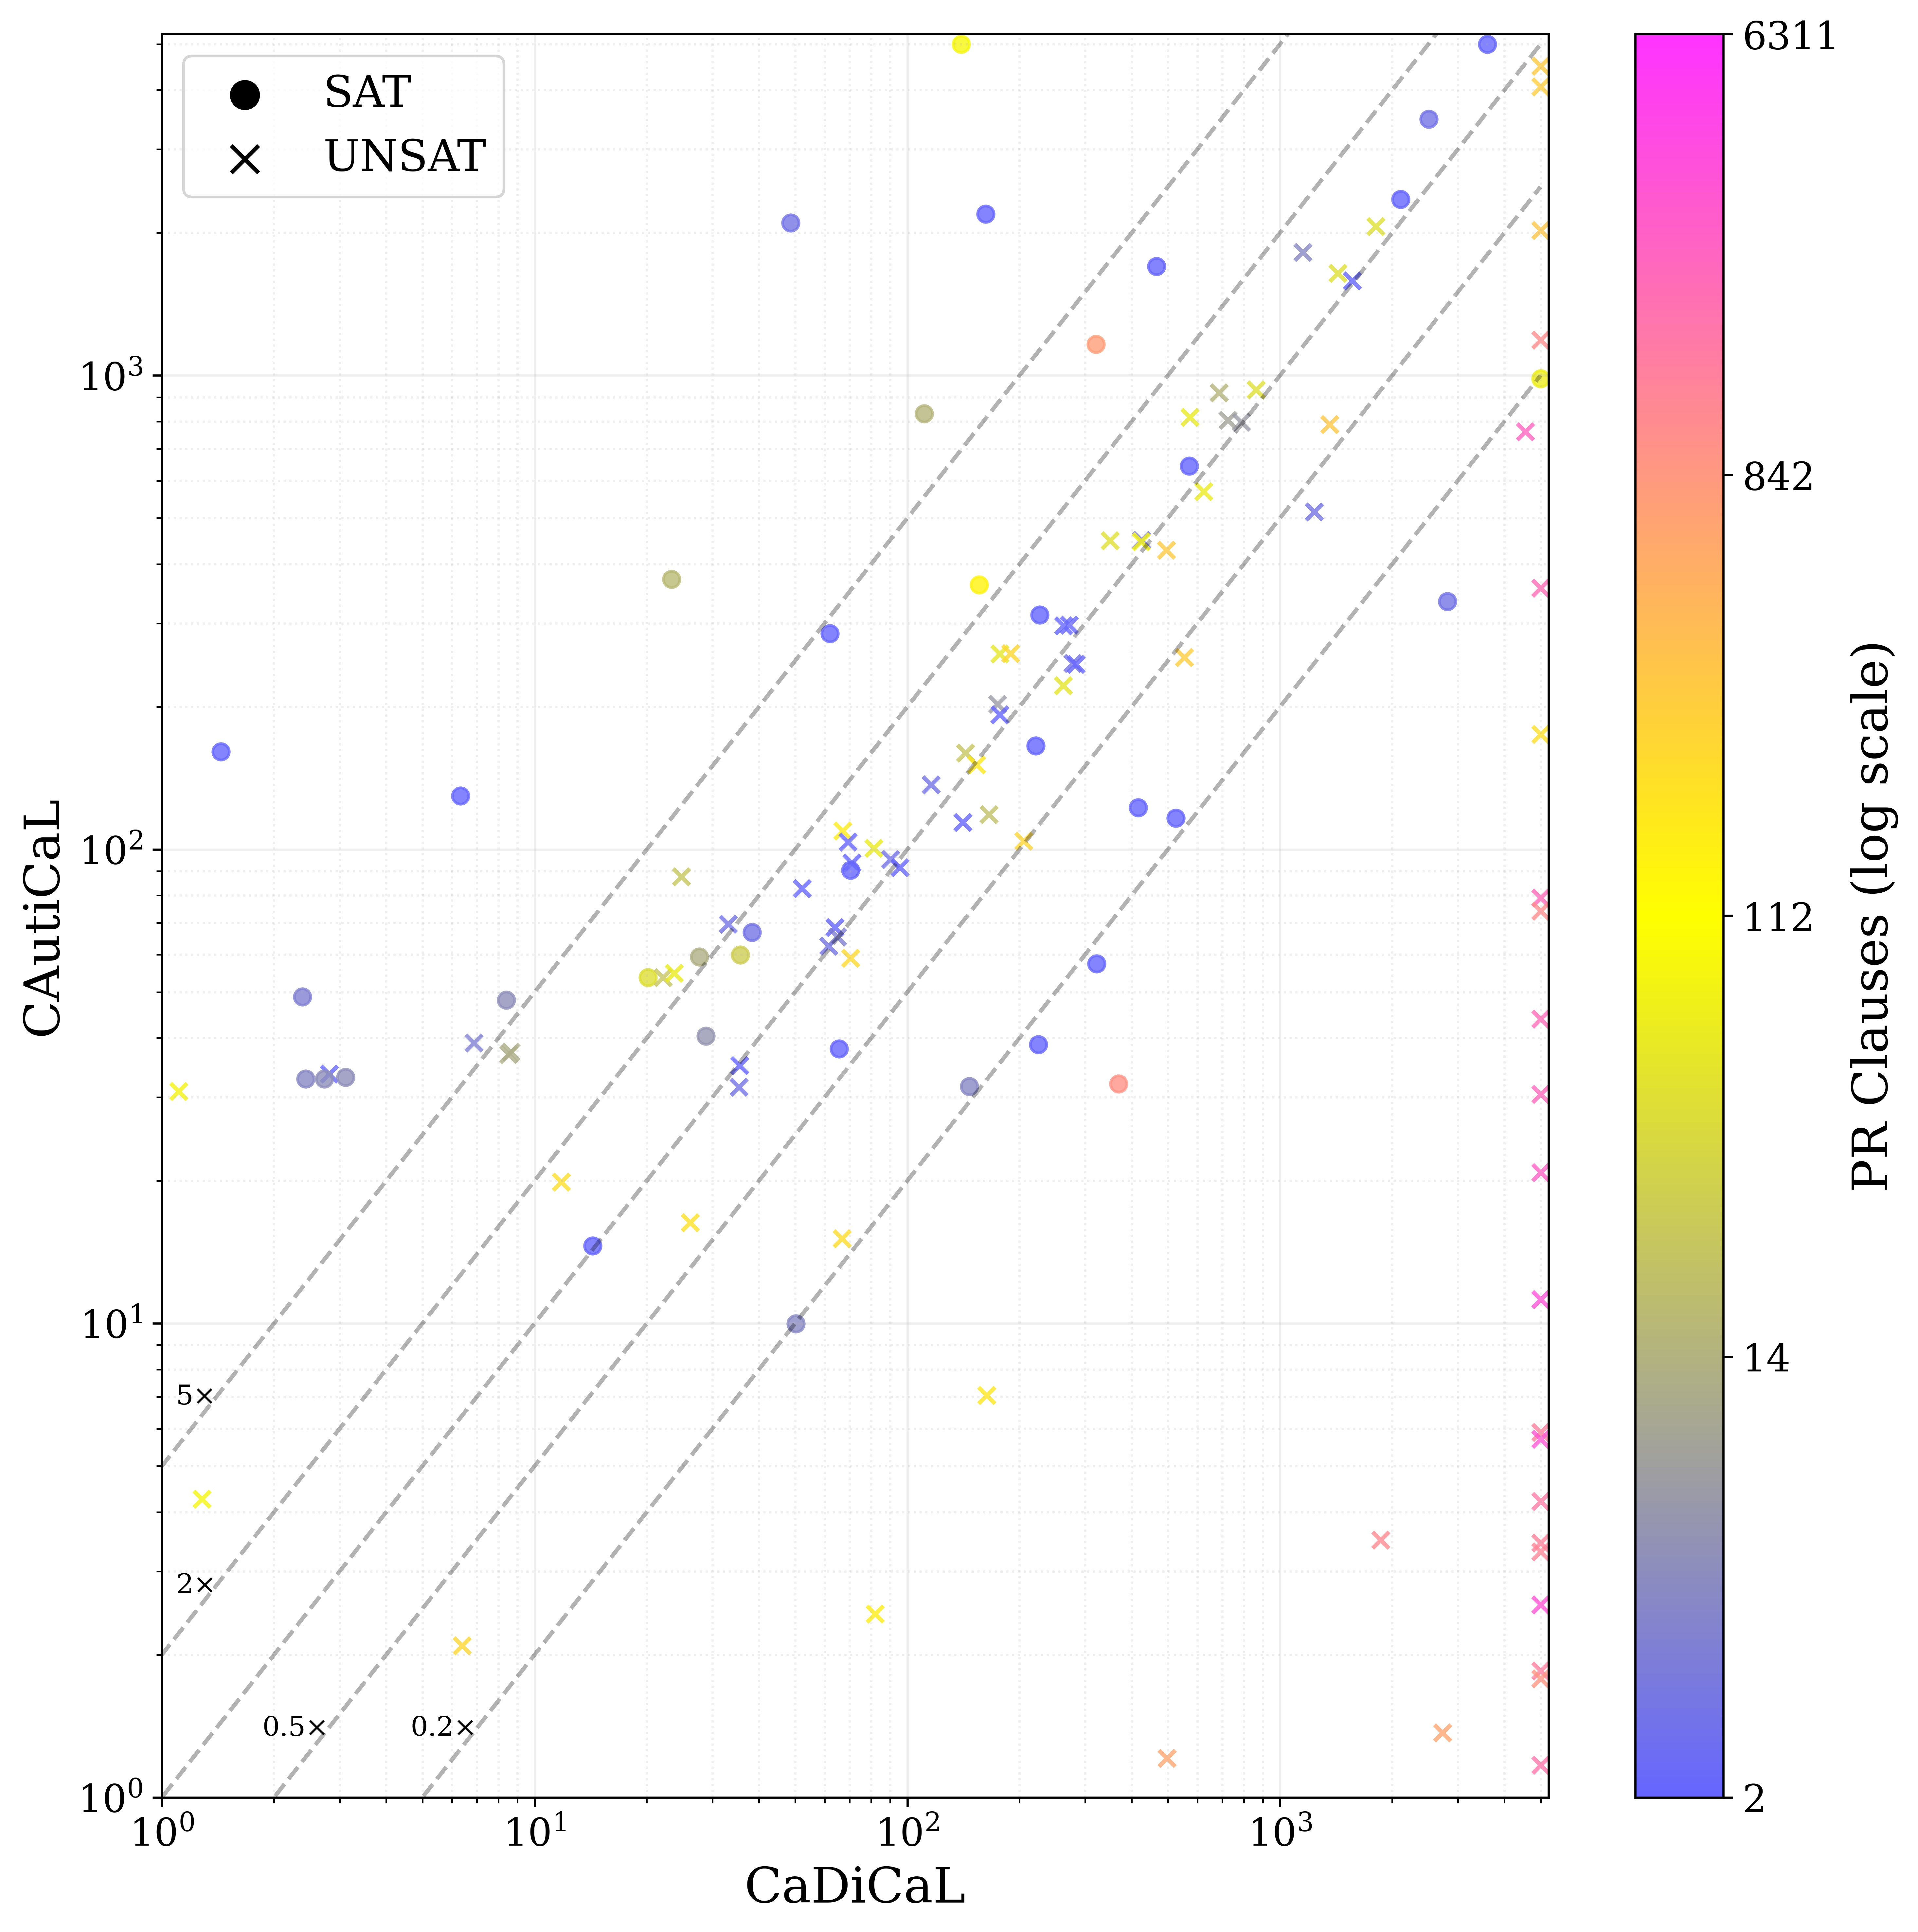
\includegraphics[width=\textwidth]{figs/cadical_vs_cautical_nontrivial.jpg}
        \caption{Comparing \tool to \cadical.}% The color indicates the number
        % of \pr clauses learnt by \tool}
        \label{subfig:cautical-vs-cadical-satcomp}
    \end{subfigure}
    \hspace{0.06\textwidth}
    % \begin{subfigure}[t]{0.45\textwidth} \centering
    %     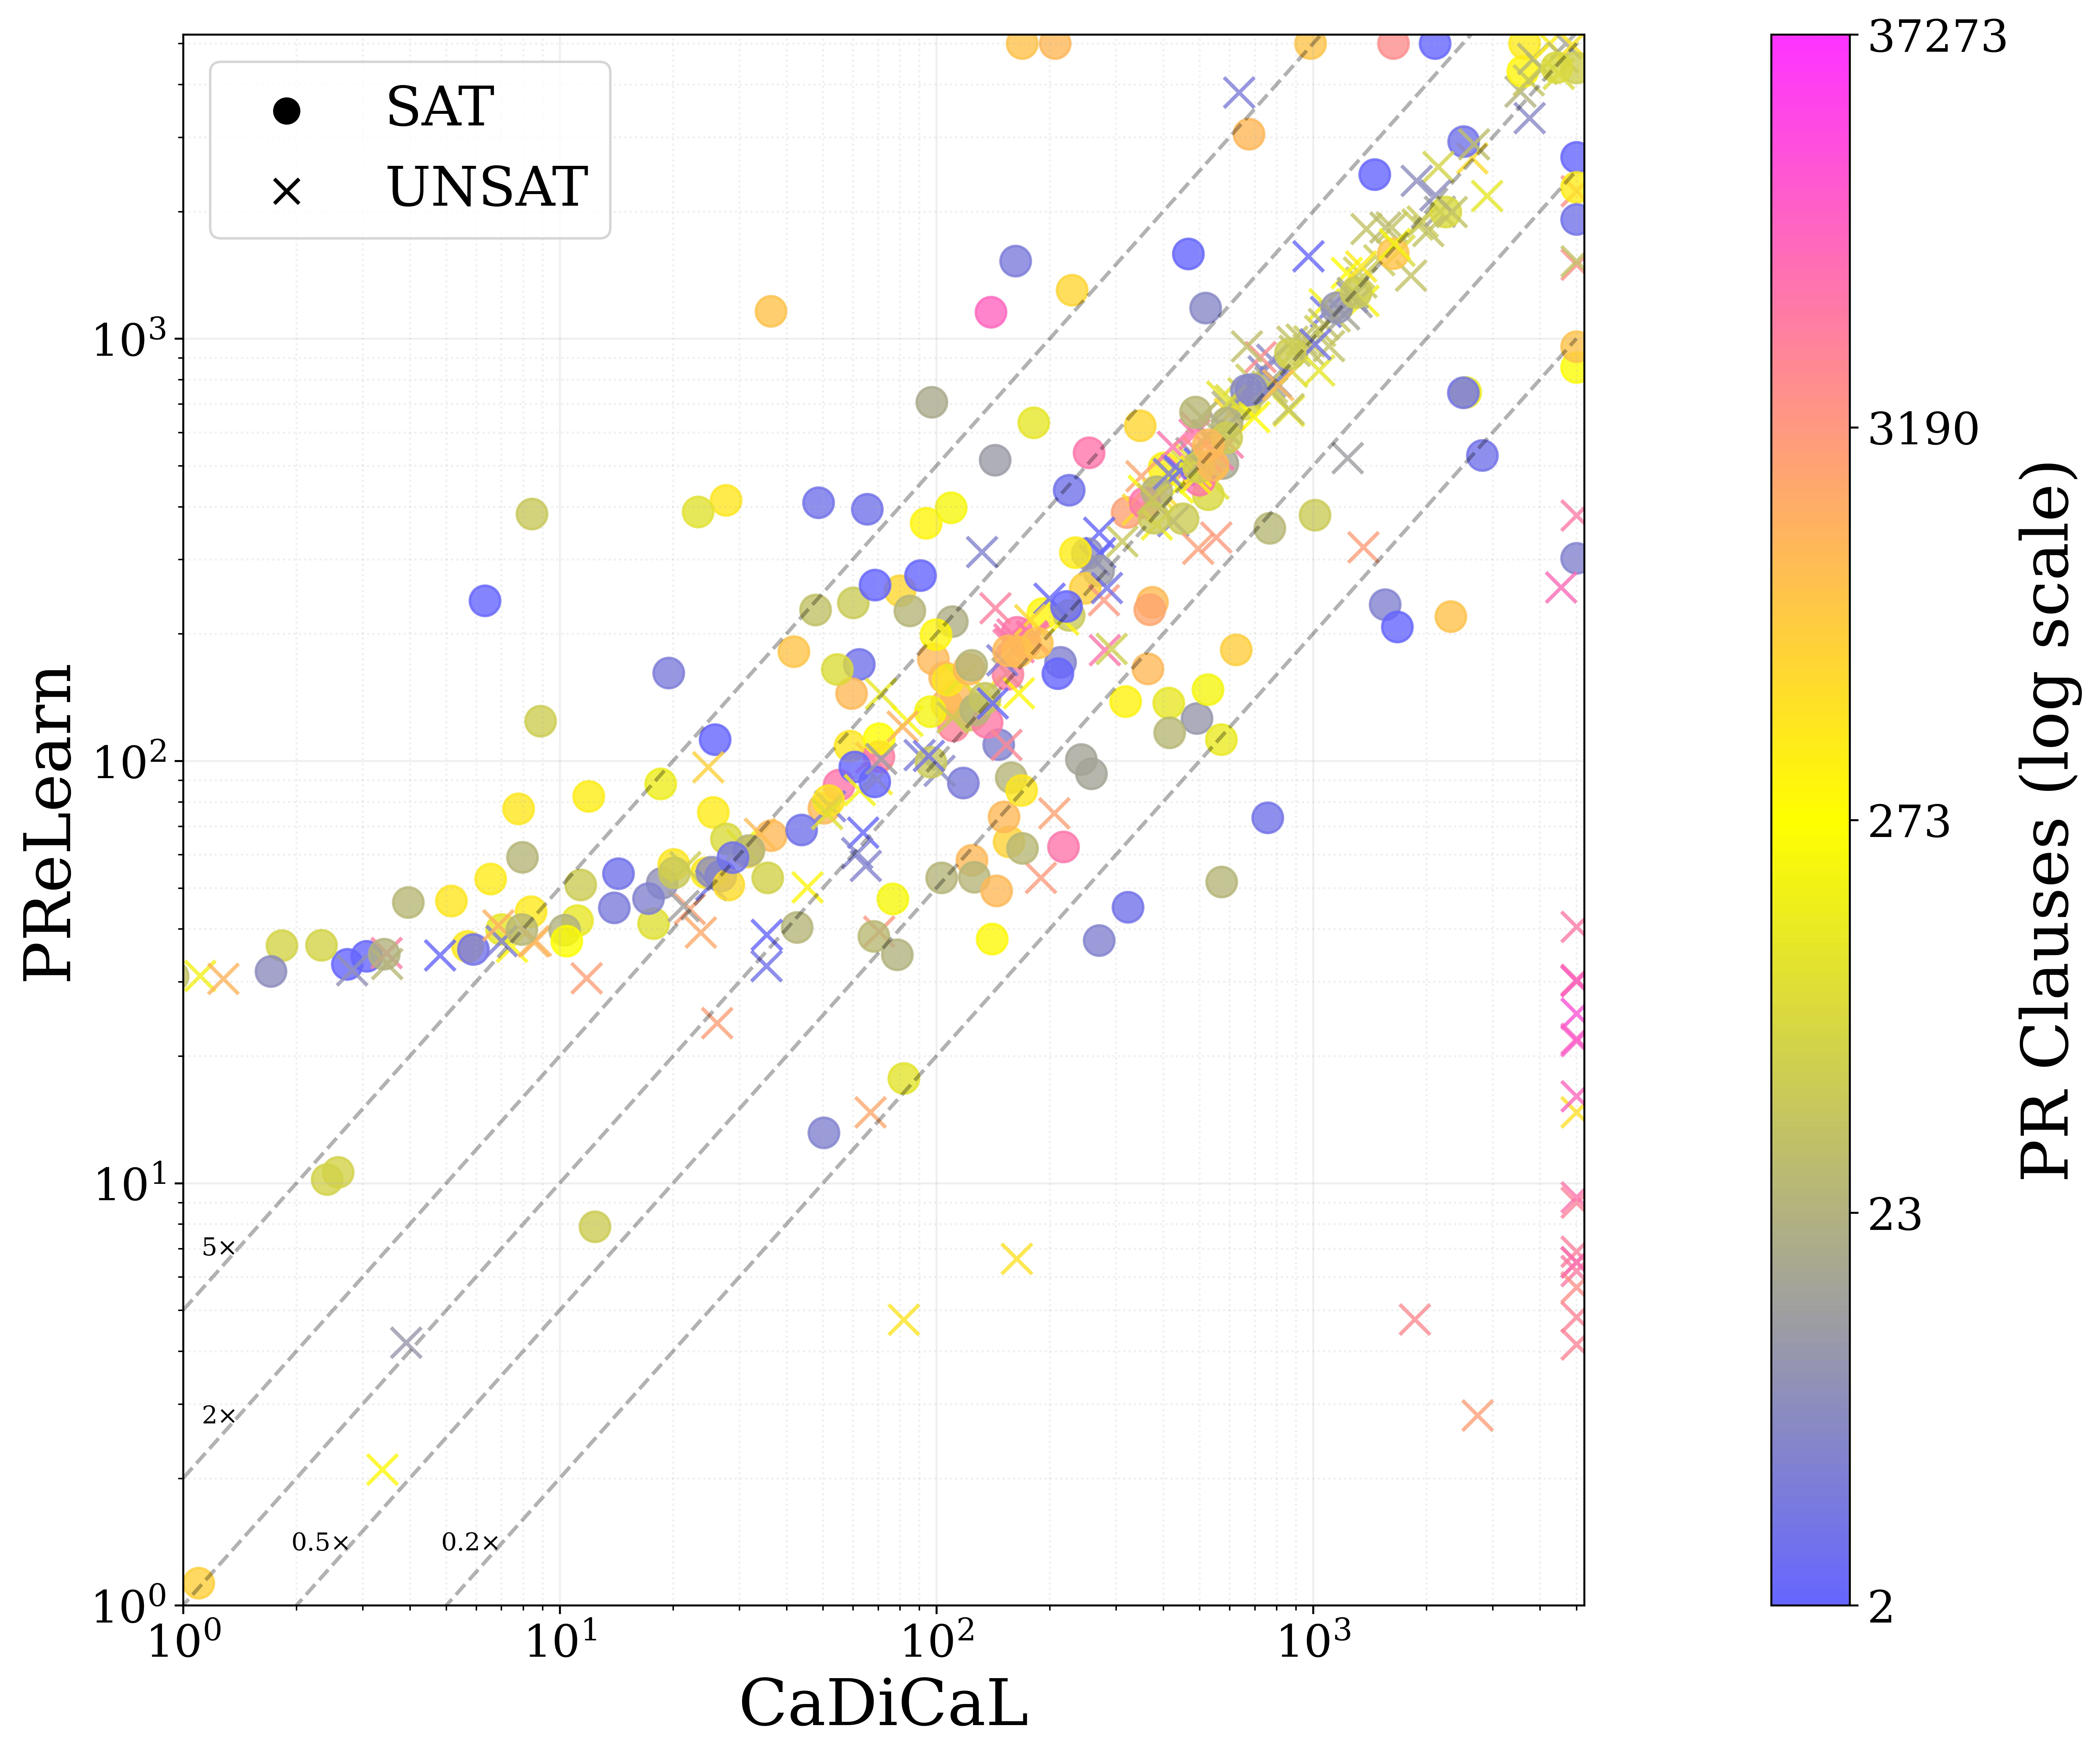
\includegraphics[width=\textwidth]{figs/cadical_vs_prelearn_nontrivial.jpg}
    %     \caption{Comparing \prelearn to \cadical. The color indicates the
    %     number of \pr clauses learnt by \prelearn}
    %     \label{subfig:cautical-vs-prelearn-satcomp} \end{subfigure}
    \begin{subfigure}[t]{0.45\textwidth}
        \centering
        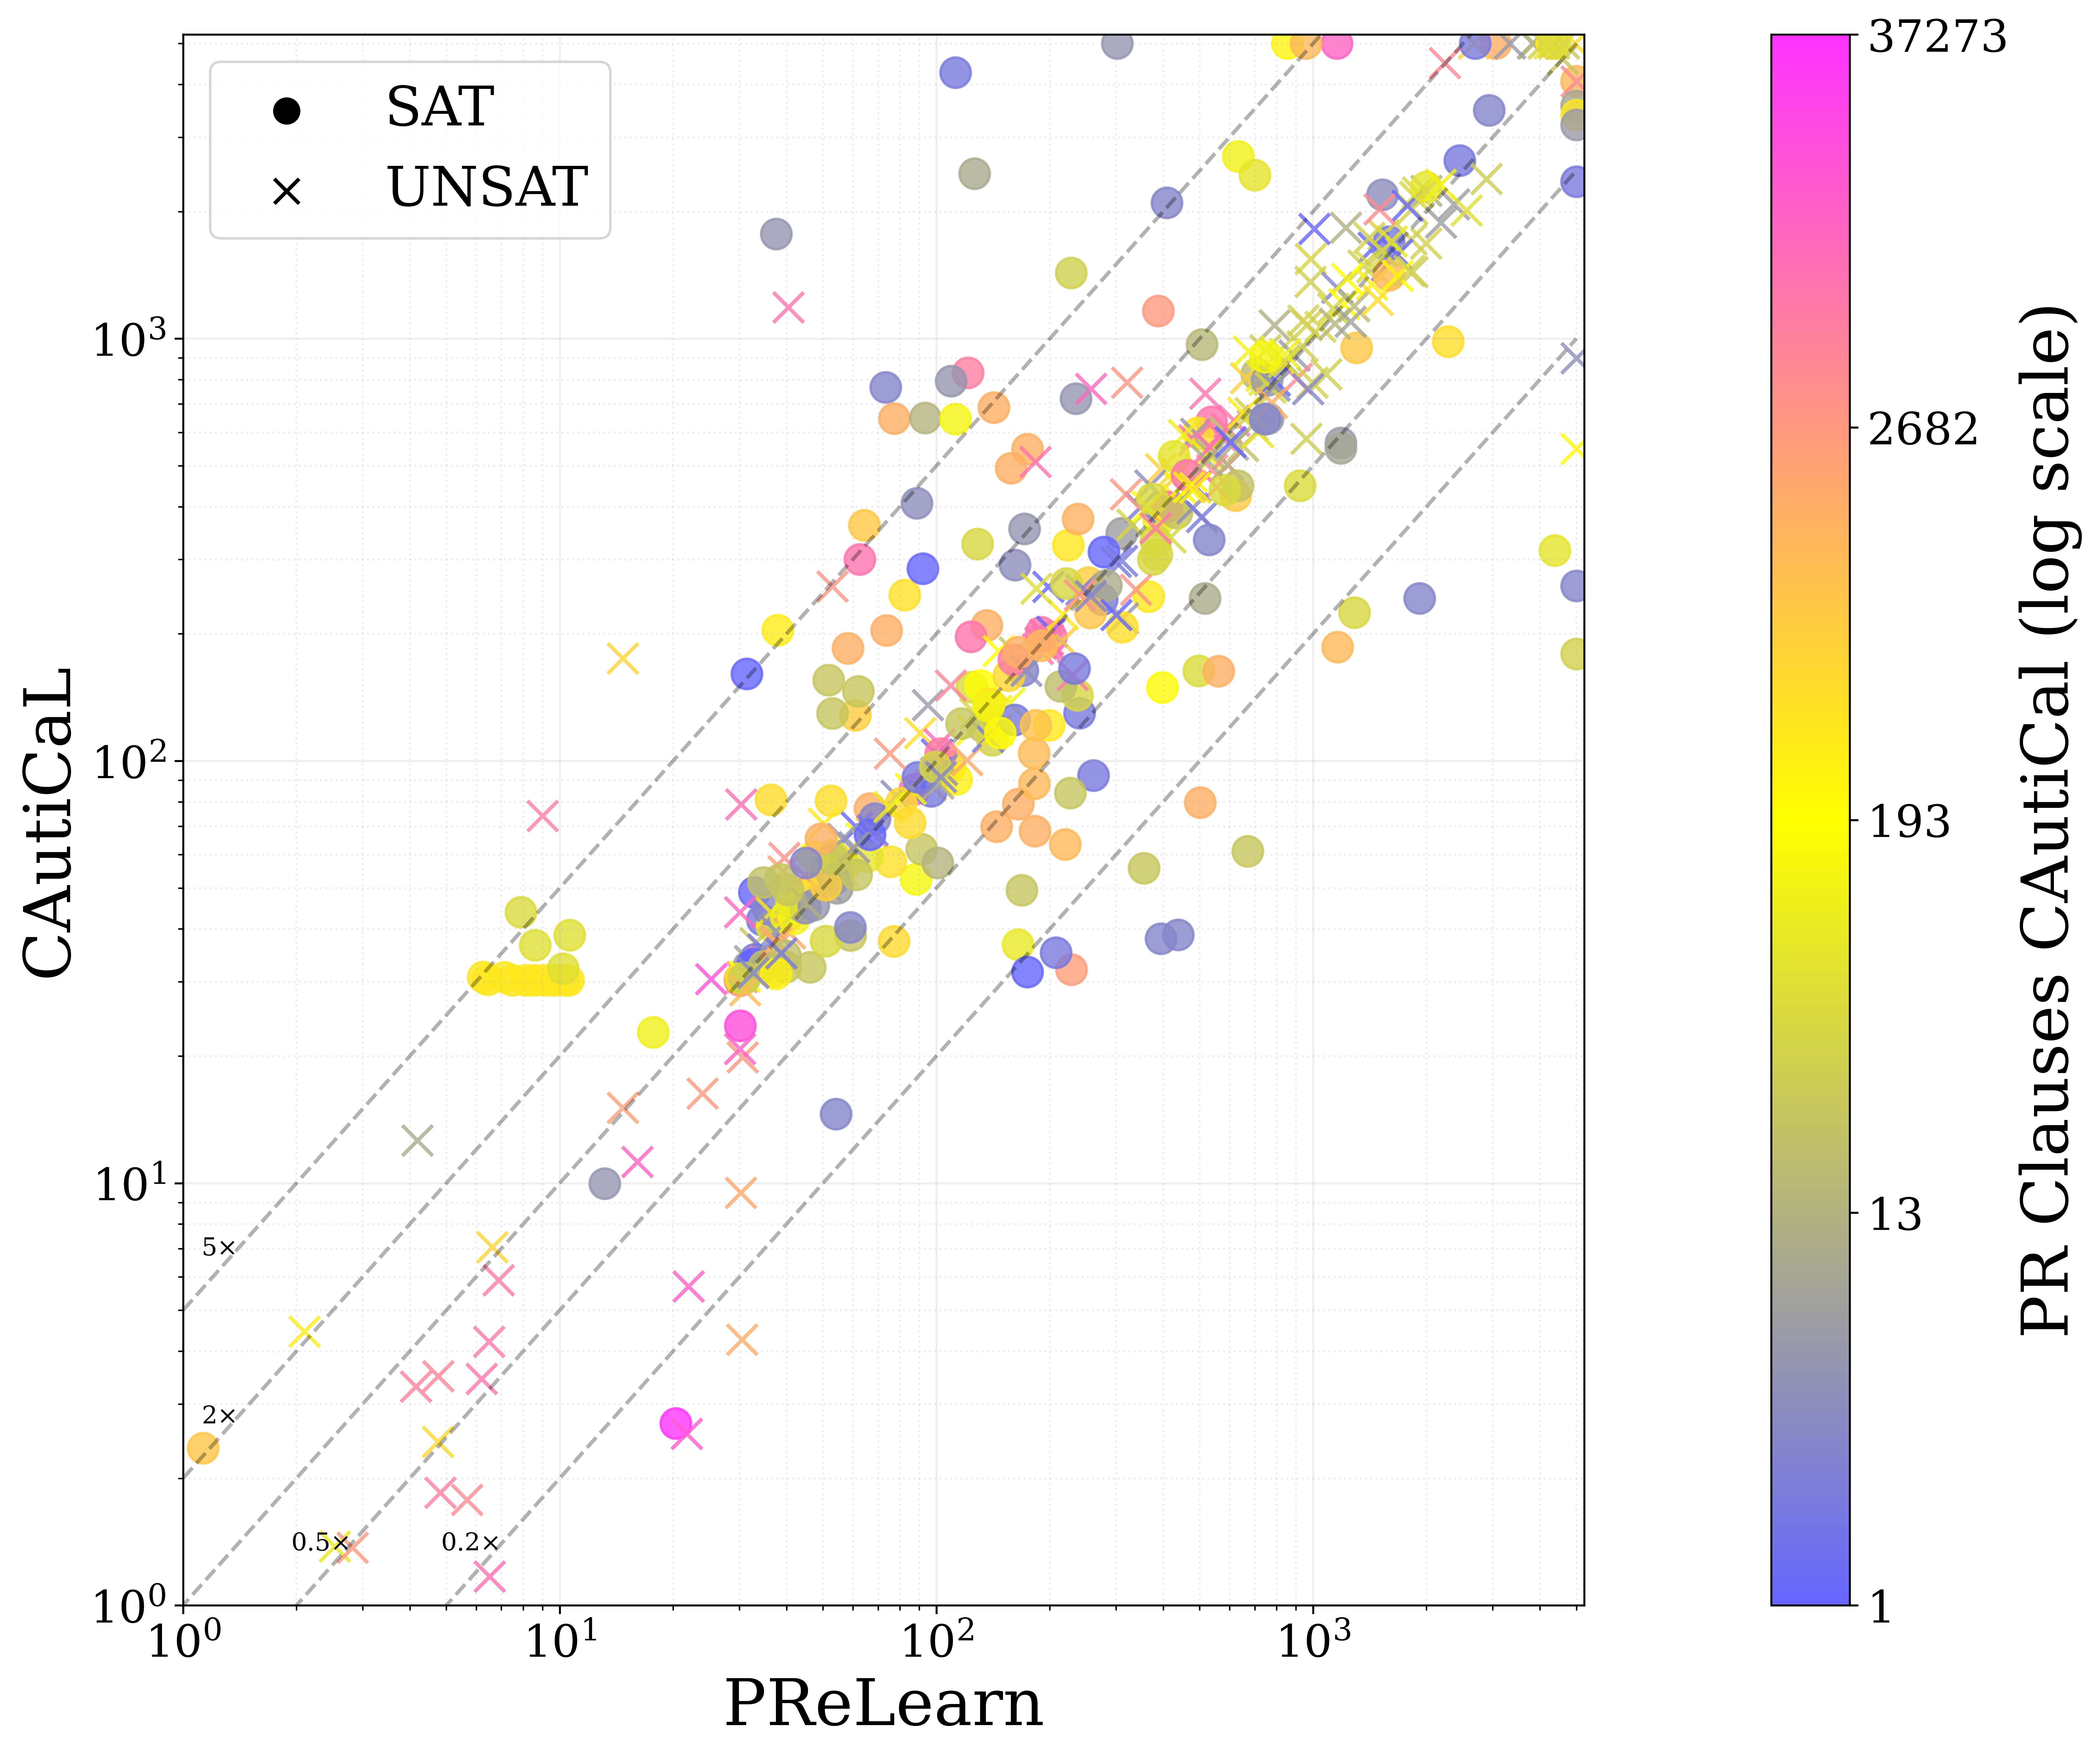
\includegraphics[width=\textwidth]{figs/prelearn_vs_cautical_nontrivial.jpg}
        \subcaption{Comparing \tool to \prelearn.}% The color
        % indicates the number of \pr clauses learnt by \tool. We filter out all
        % formula where neither \tool nor \prelearn learnt any \pr clauses.}
        \label{subfig:cautical-vs-prelearn-performance}
    \end{subfigure}
    % \caption{Performance comparison of \tool with and \prelearn with \cadical
    % on SAT competition benchmarks. We filter out all benchmarks where each
    % solver does not learn any \pr clauses. The color indicates the number of
    % \pr clauses learnt.}
    \caption{Performance comparison of \tool with \prelearn and \cadical on SAT competition benchmarks. On each graph, we filter out all benchmarks where neither solver learns any \pr clauses. The color indicates the number of \pr clauses learnt by \tool.}
    \label{fig:solver-comparison}
\end{figure*}

\begin{table}[h]
    \centering
    \sisetup{table-format=3}        % remove if you are not using siunitx
    \begin{tabular}{lrrrrr}
      \toprule
      & \multicolumn{2}{c}{0--10k clause} & \multicolumn{2}{c}{10k--20M clause}
      \\
      \cmidrule(lr){2-3} \cmidrule(lr){4-5} & SAT & UNSAT & SAT & UNSAT & Total
      \\
      \midrule
    %   Total Formulas & 70 & 132 & 395 & 416 & 1099 \\
      \cadical Solved  &  54 &  73 & 319 & 303 & 749 \\
      \midrule
      \prelearn \\
      \; Total &  52 &  90 & 322 & 307 & 771 \\
      \; Learn \pr clause   &  40 &  73 & 179 & 145 & 431\\
      \; Learn $>50$ \pr clauses   &  22 &  51 & 104 &  79 & 256\\
      \; Improve on \cadical &  11 &  42 &  57 &  36 & 146\\
      \; Unique from \cadical &   1 &  17 &   6 &   6 & 30 \\
      \midrule
      \tool \\
      \; Total &  52 &  87 & 317 & 298 & 754 \\
      \; Learn \pr clause     &   16 &  58 &  30 &  35 & 139 \\
      \; Learn $>$$50$ \pr clauses  &   1  &  39 &  6 &  11 & 57 \\
      \; Improve on \cadical &  23  &  48 &  89 &  59 & 219 \\
      \; Unique from \cadical &   0 &  18 &   9 &   9 & 36 \\
      \bottomrule
    \end{tabular}
    \caption{Number of formulas that \cadical, \prelearn and \tool solve, divided between 0-10k clause and 10k-20M clause formulas, and SAT and UNSAT formulas. For \prelearn and \tool we include the number of benchmarks with \pr clauses learnt, more than $50$ \pr clauses learnt, improved on \cadical by 5\% or more; and solved that \cadical did not solve.}
    \label{tab:solver-stats}
  \end{table}

\begin{figure*}[!ht]
    \centering
    \begin{minipage}[b]{0.45\textwidth}
        \centering
        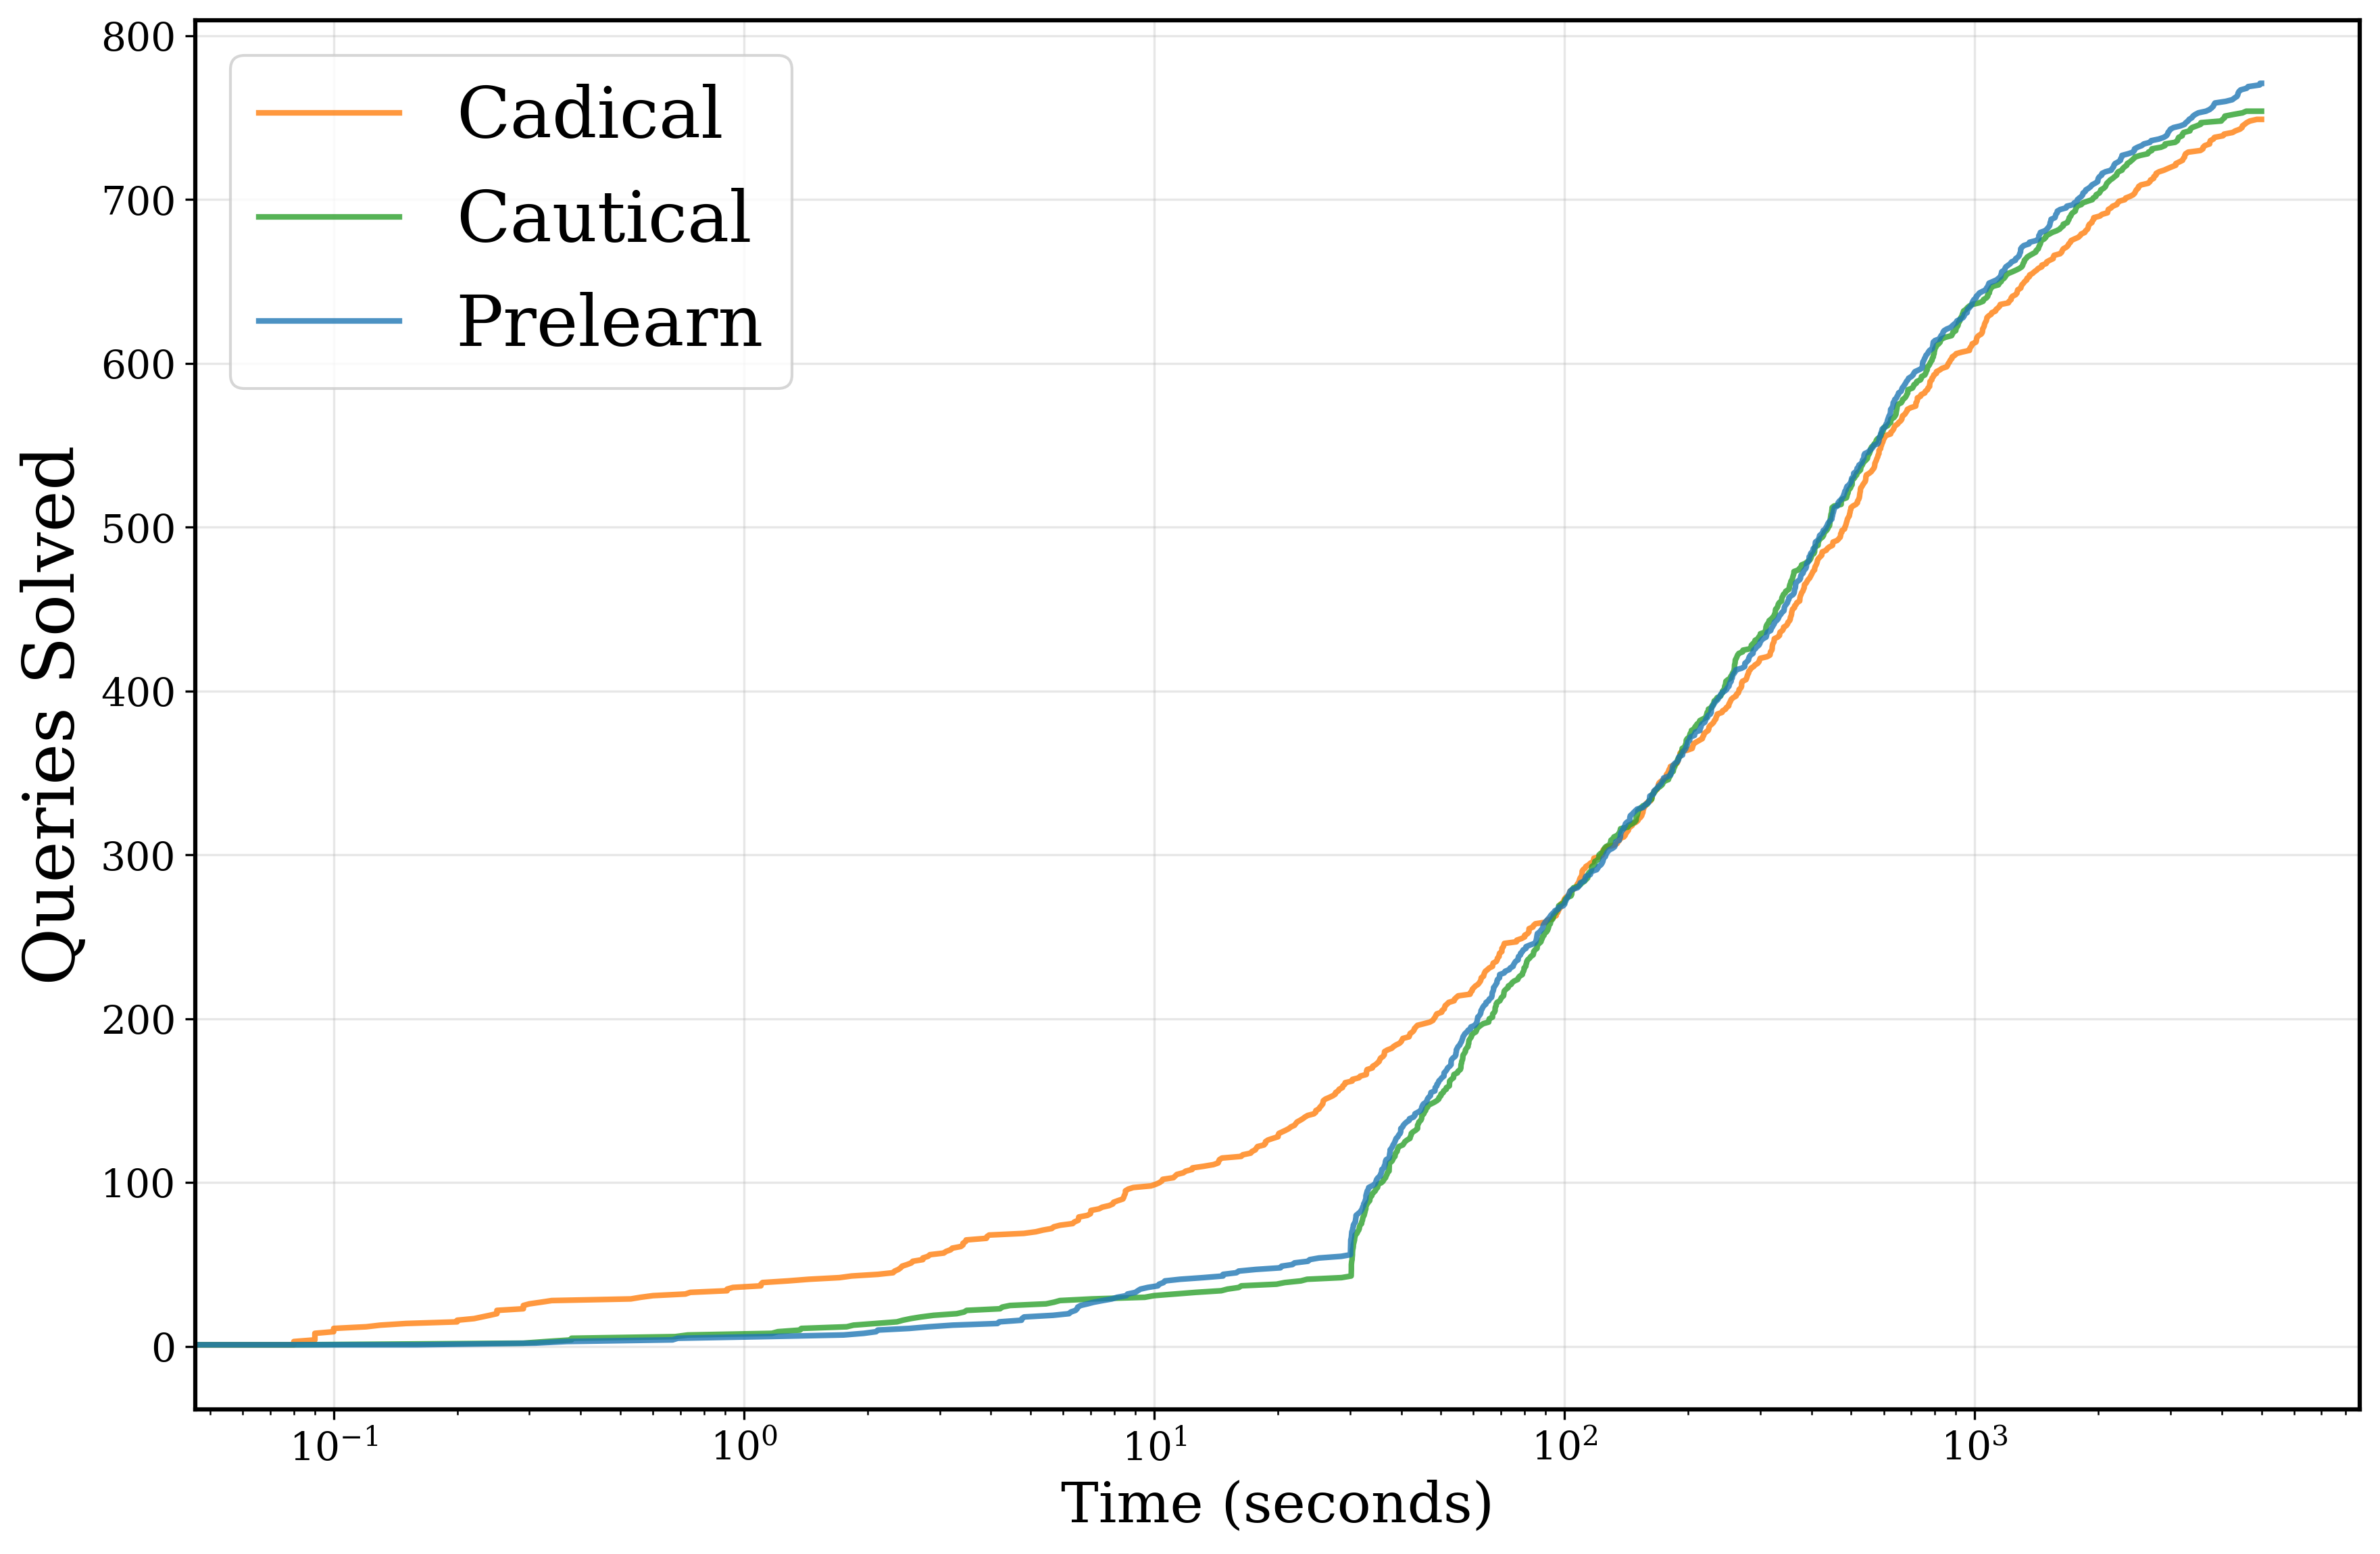
\includegraphics[width=\textwidth]{figs/cdf.png}
        \caption{CDF showing the number of formulas solved by \tool, \prelearn, and \cadical.}
        \label{fig:cdf}
    \end{minipage}
    \hspace{0.06\textwidth}
    \begin{minipage}[b]{0.45\textwidth}
        \centering
        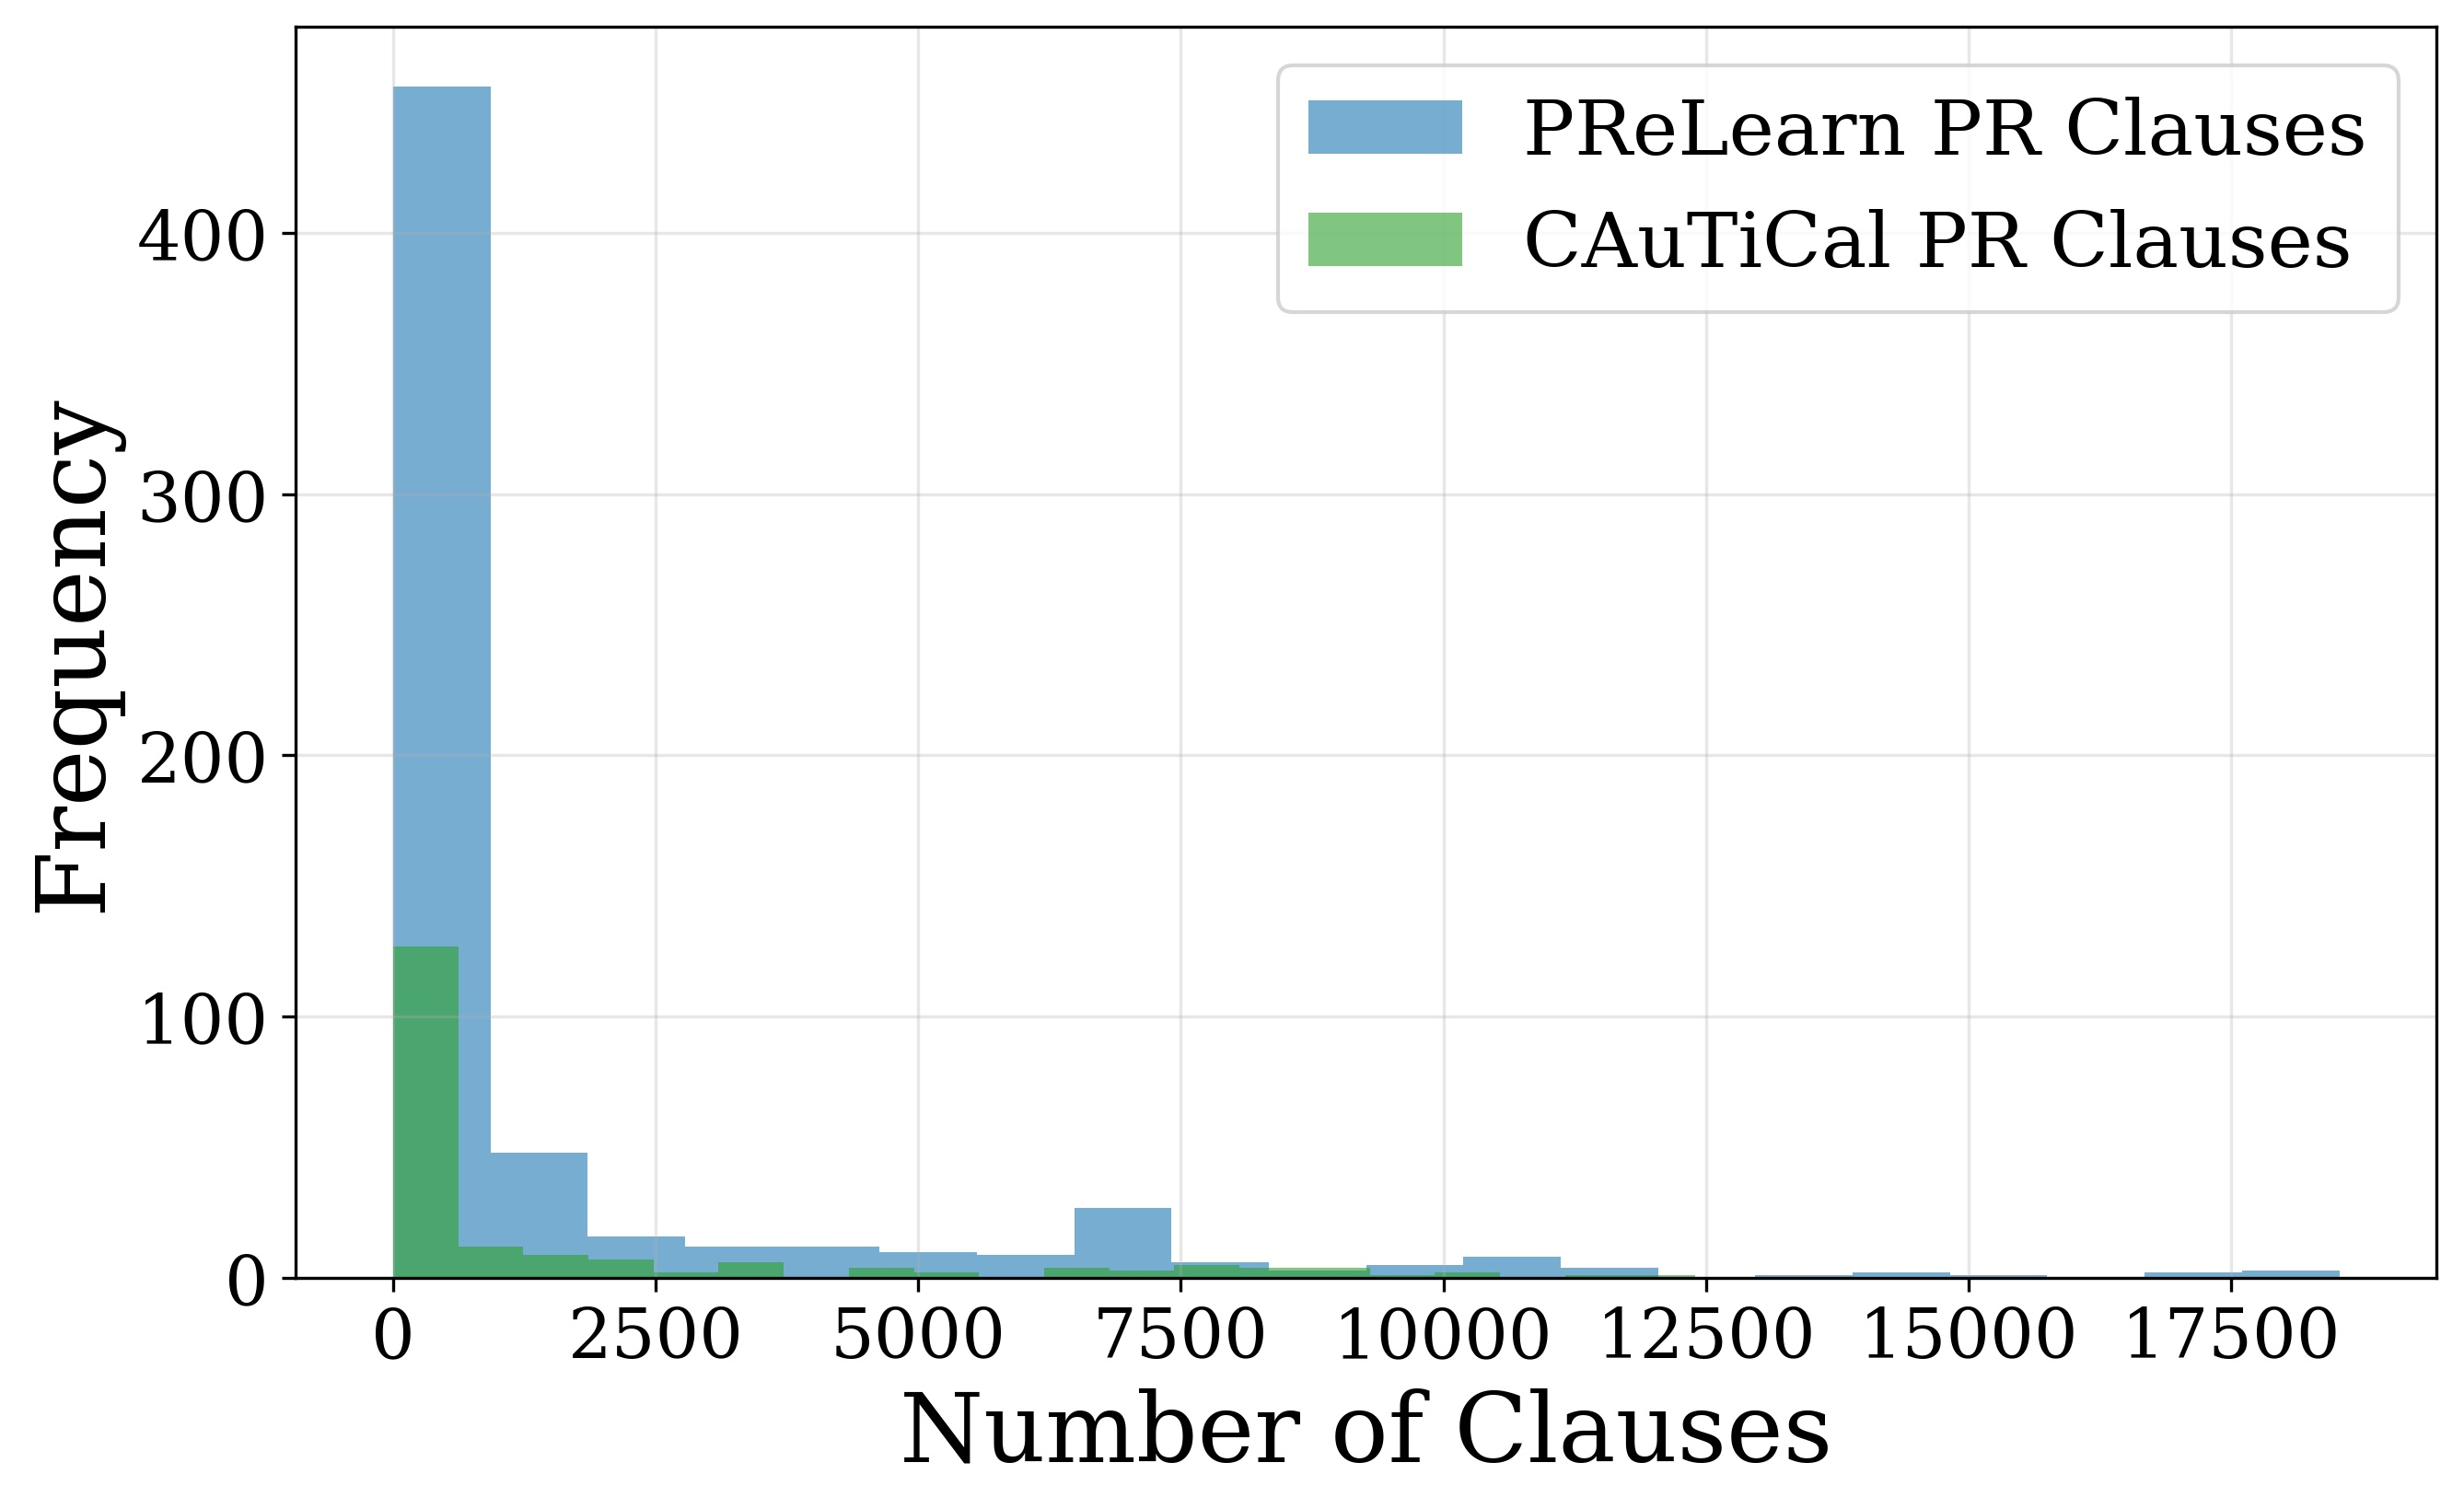
\includegraphics[width=\textwidth]{figs/clauses_histogram.jpg}
        \caption{Histogram showing the number of \pr clauses learnt by \tool and \prelearn}
        \label{fig:clauses-histogram}
    \end{minipage}
\end{figure*}

\begin{figure*}[!h]
    \centering
    \begin{subfigure}[t]{0.45\textwidth}
            \centering
            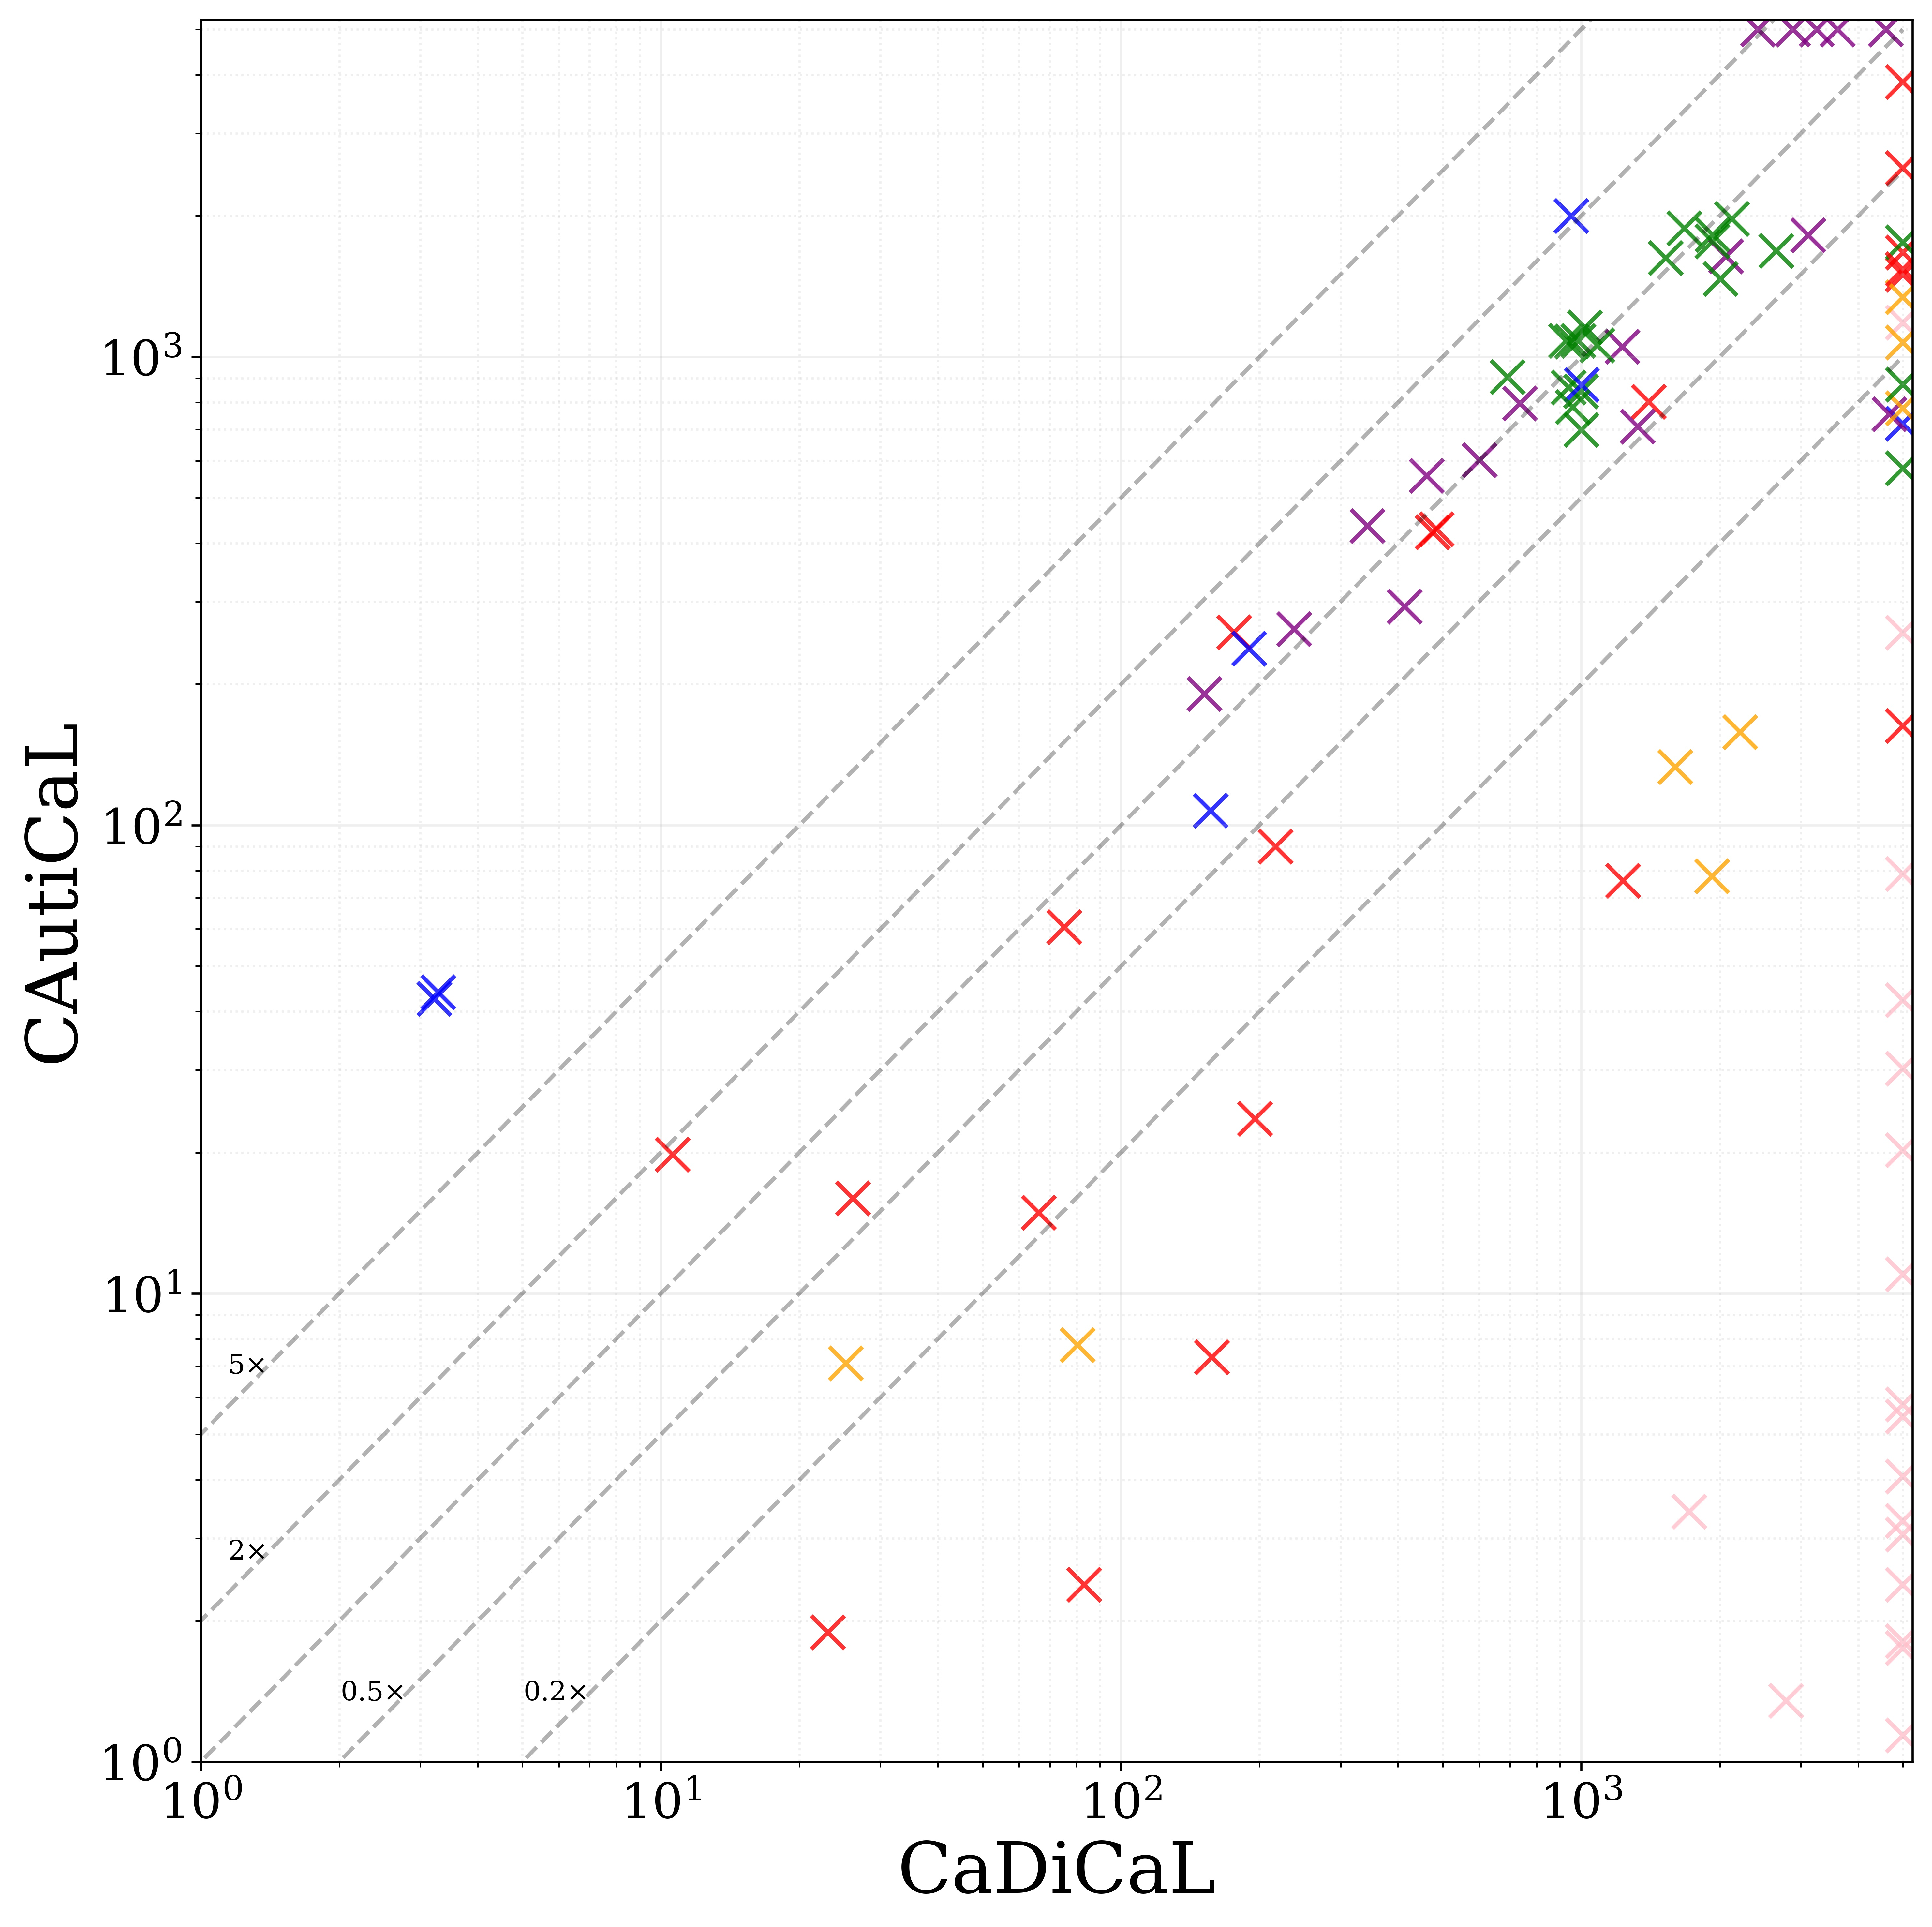
\includegraphics[width=\textwidth]{figs/cadical_vs_cautical_interesting.jpg}
            % \caption{Comparison with \cadical}
            \label{fig:cautical-vs-cadical}
    \end{subfigure}
        % \hspace{0.06\textwidth}
    % \hspace{0.06\textwidth} \begin{subfigure}[t]{0.3\textwidth} \centering
    % 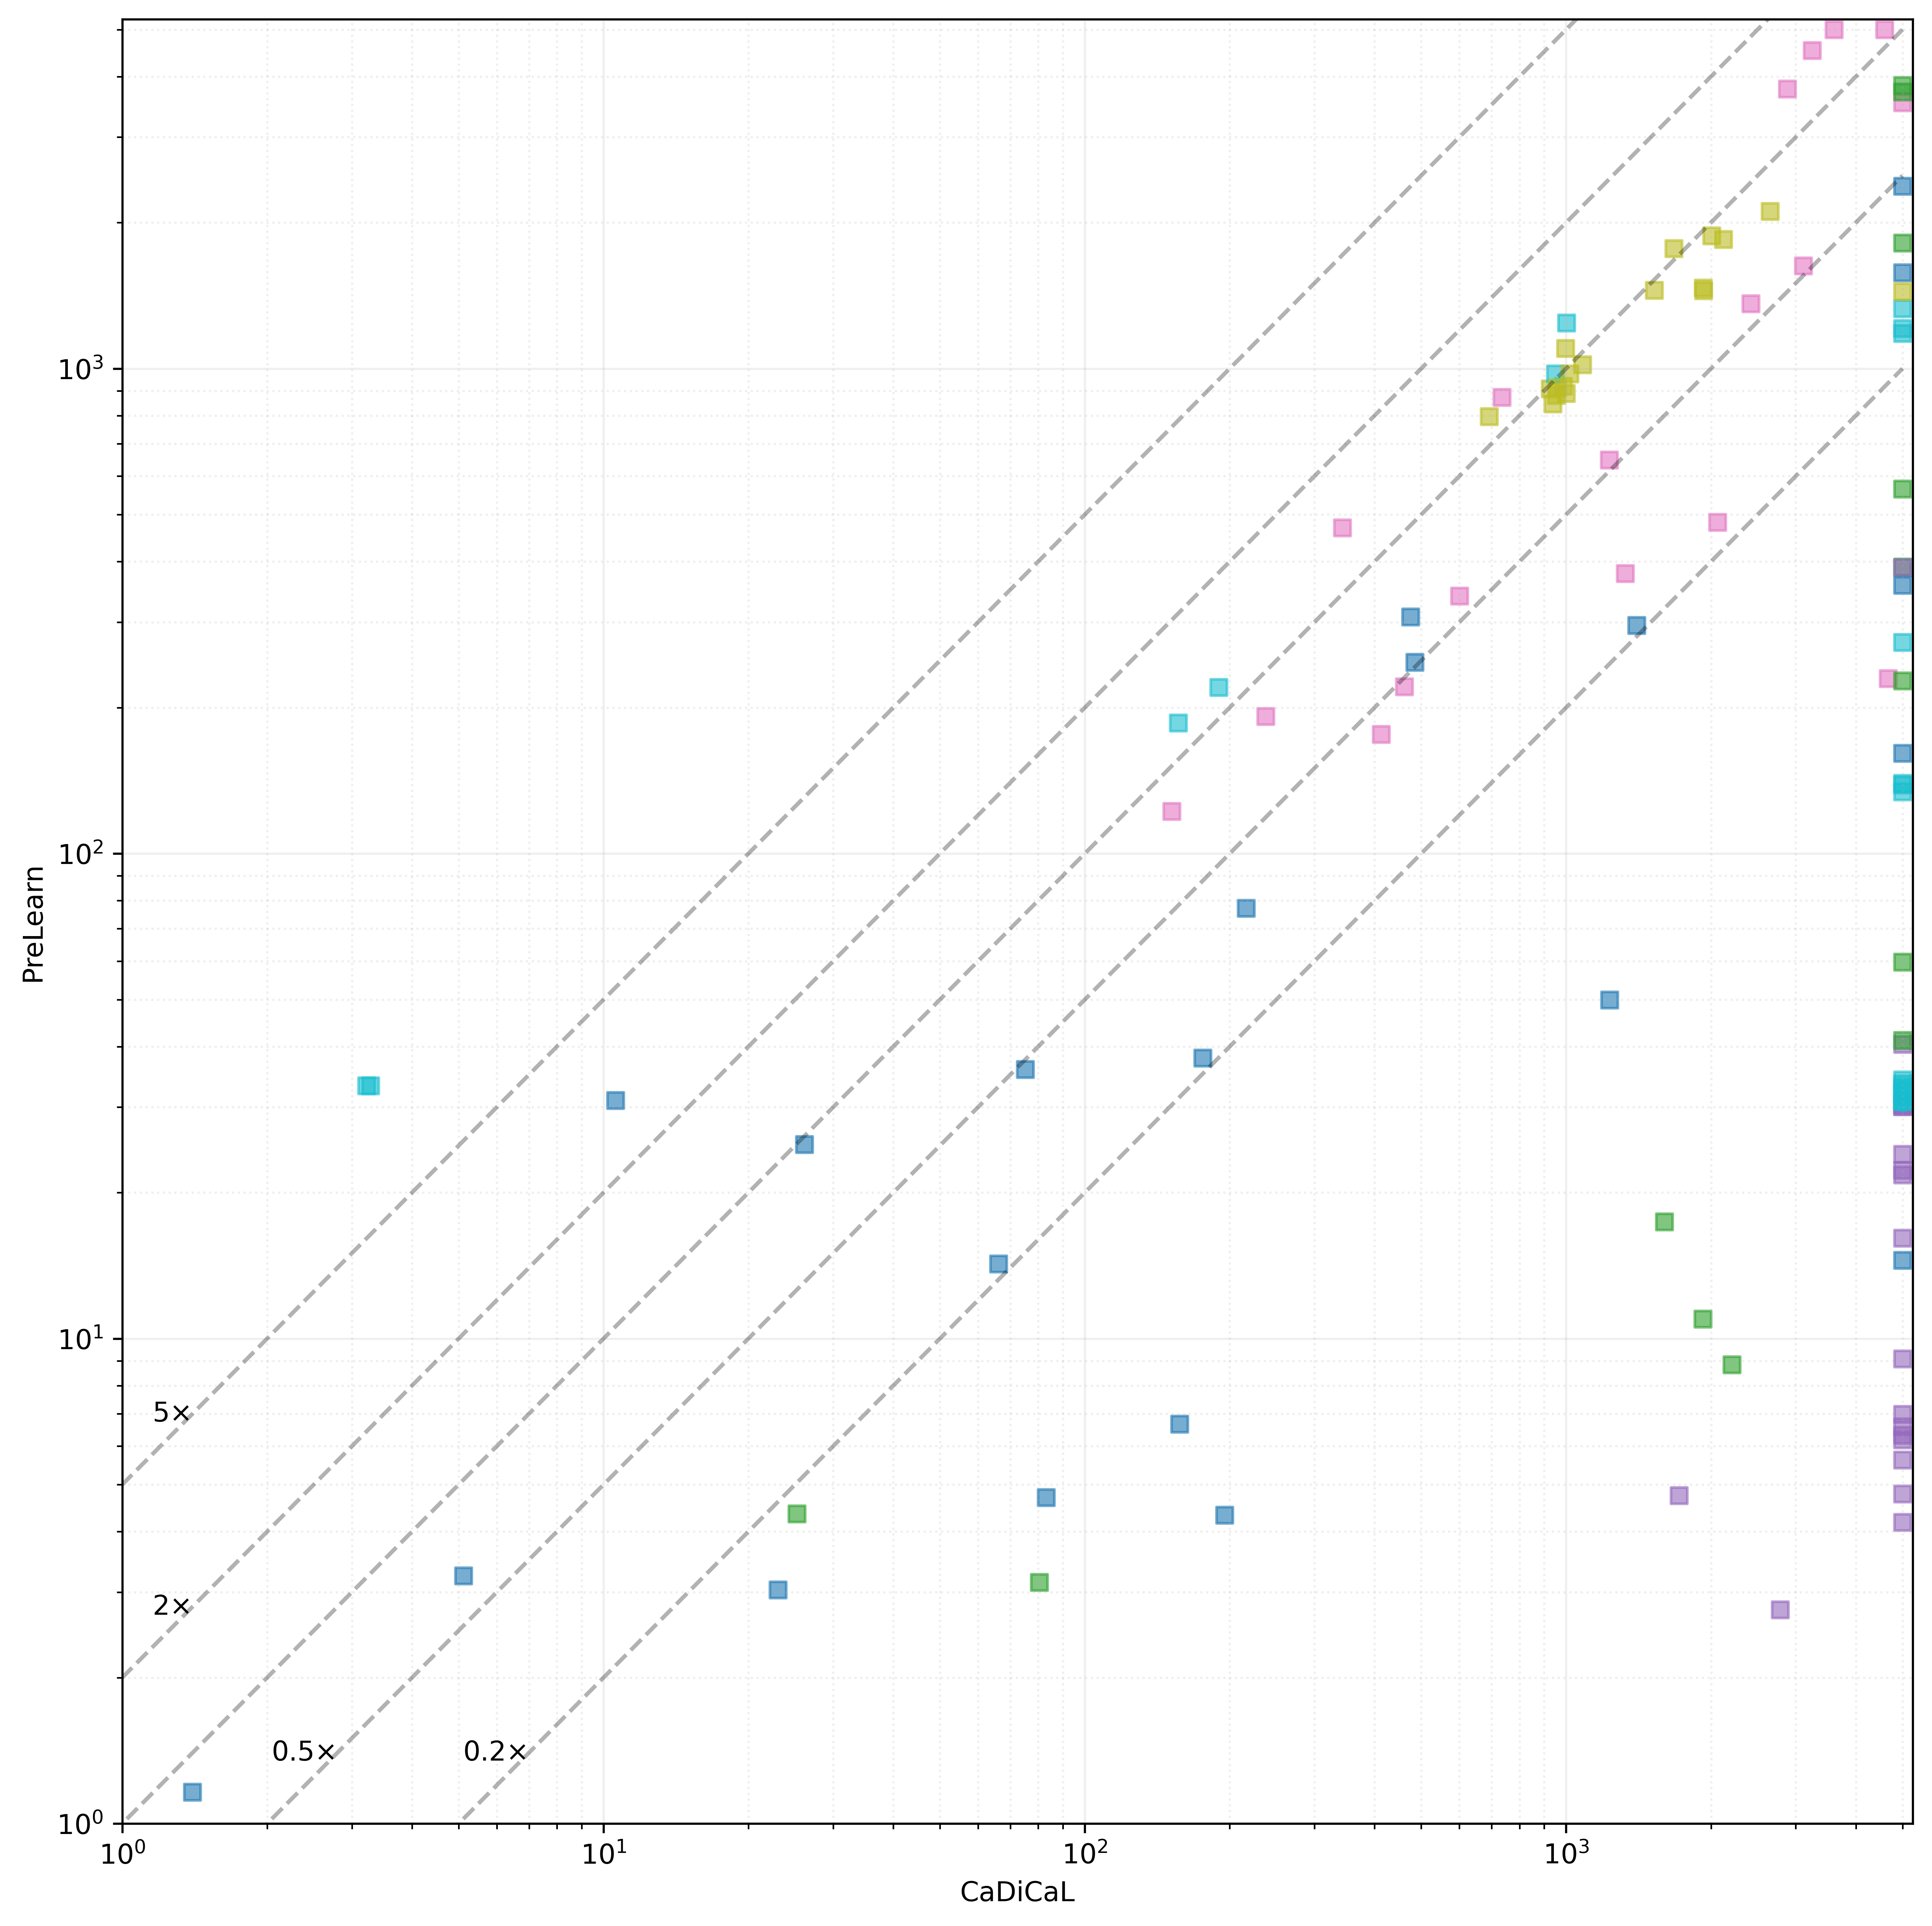
\includegraphics[width=\textwidth]{figs/prelearn_vs_cadical_interesting.jpg}
    % \caption{Comparison with \prelearn} \label{fig:cautical-vs-prelearn}
    % \end{subfigure}
    \begin{subfigure}[t]{0.45\textwidth}
        \centering
        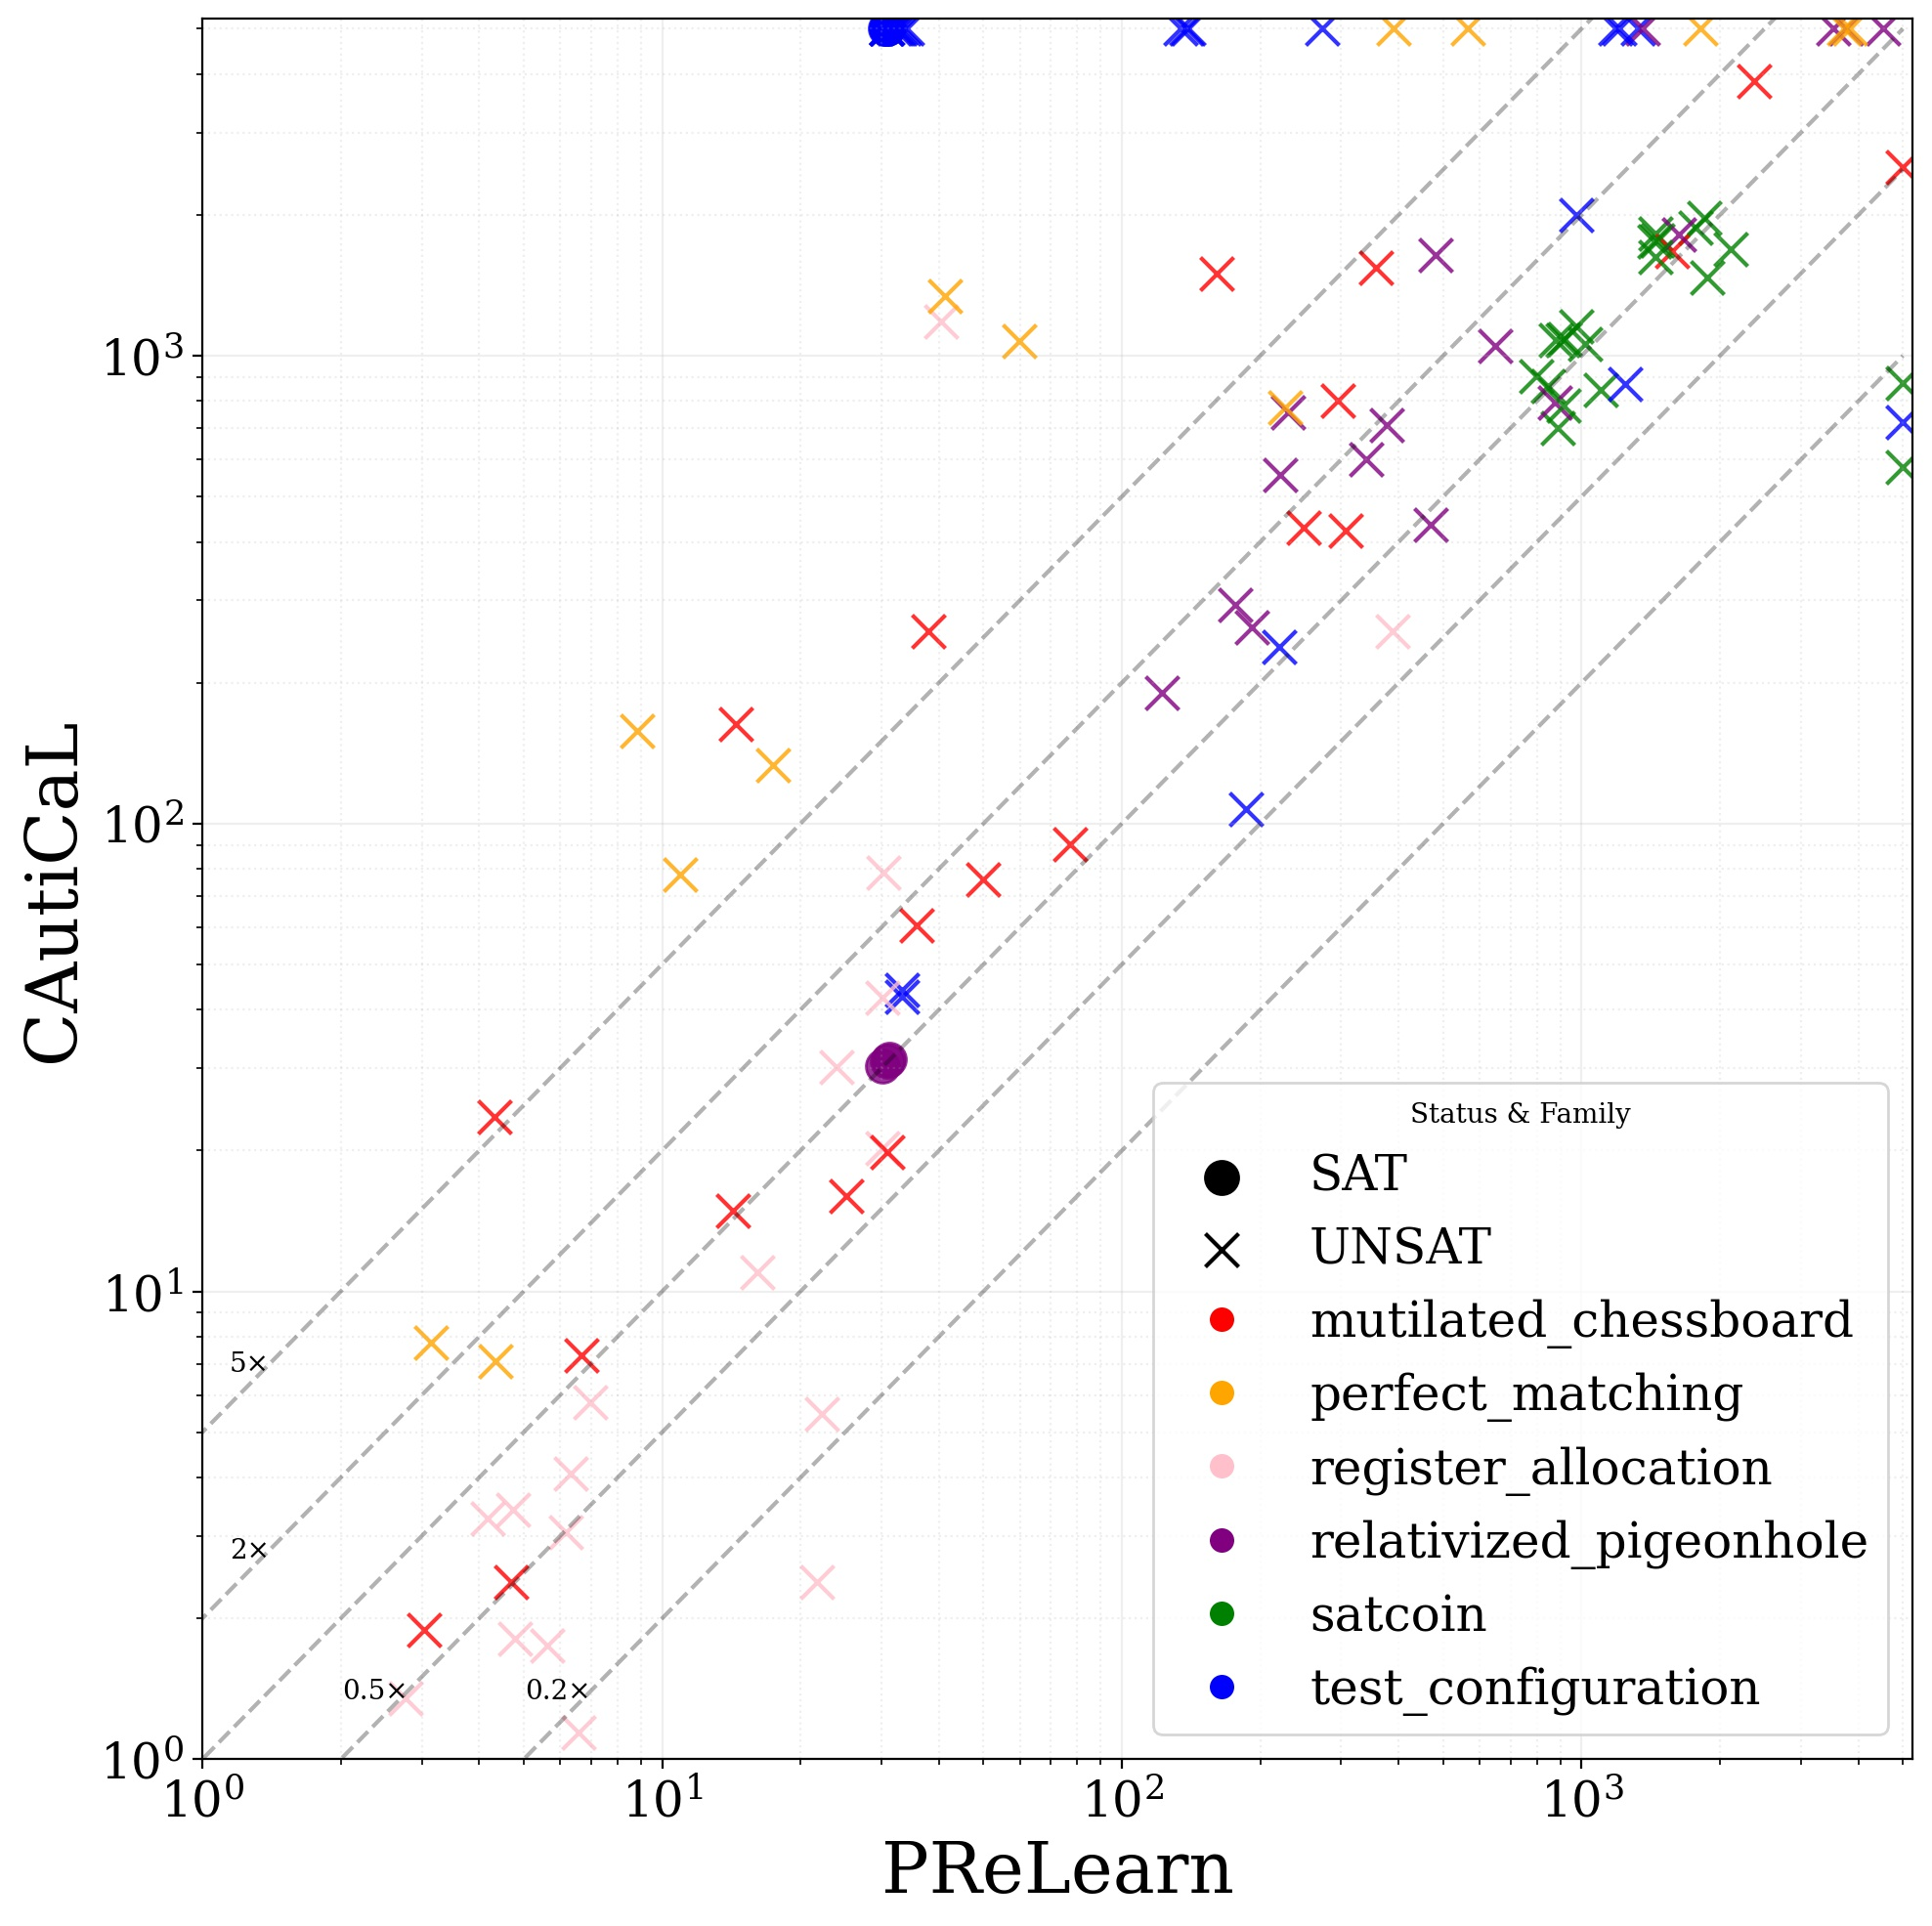
\includegraphics[width=\textwidth]{figs/prelearn_vs_cautical_interesting_legend.jpg}
        % \caption{Comparison with \prelearn}
        \label{fig:cautical-vs-prelearn}
    \end{subfigure}

    \caption{Comparing \tool with \cadical and \prelearn on various benchmark families.}
    \label{fig:solver-comparison-familis}
\end{figure*}

\begin{figure*}[!t]
    \centering
    \begin{subfigure}[t]{0.3\textwidth}
    \centering
    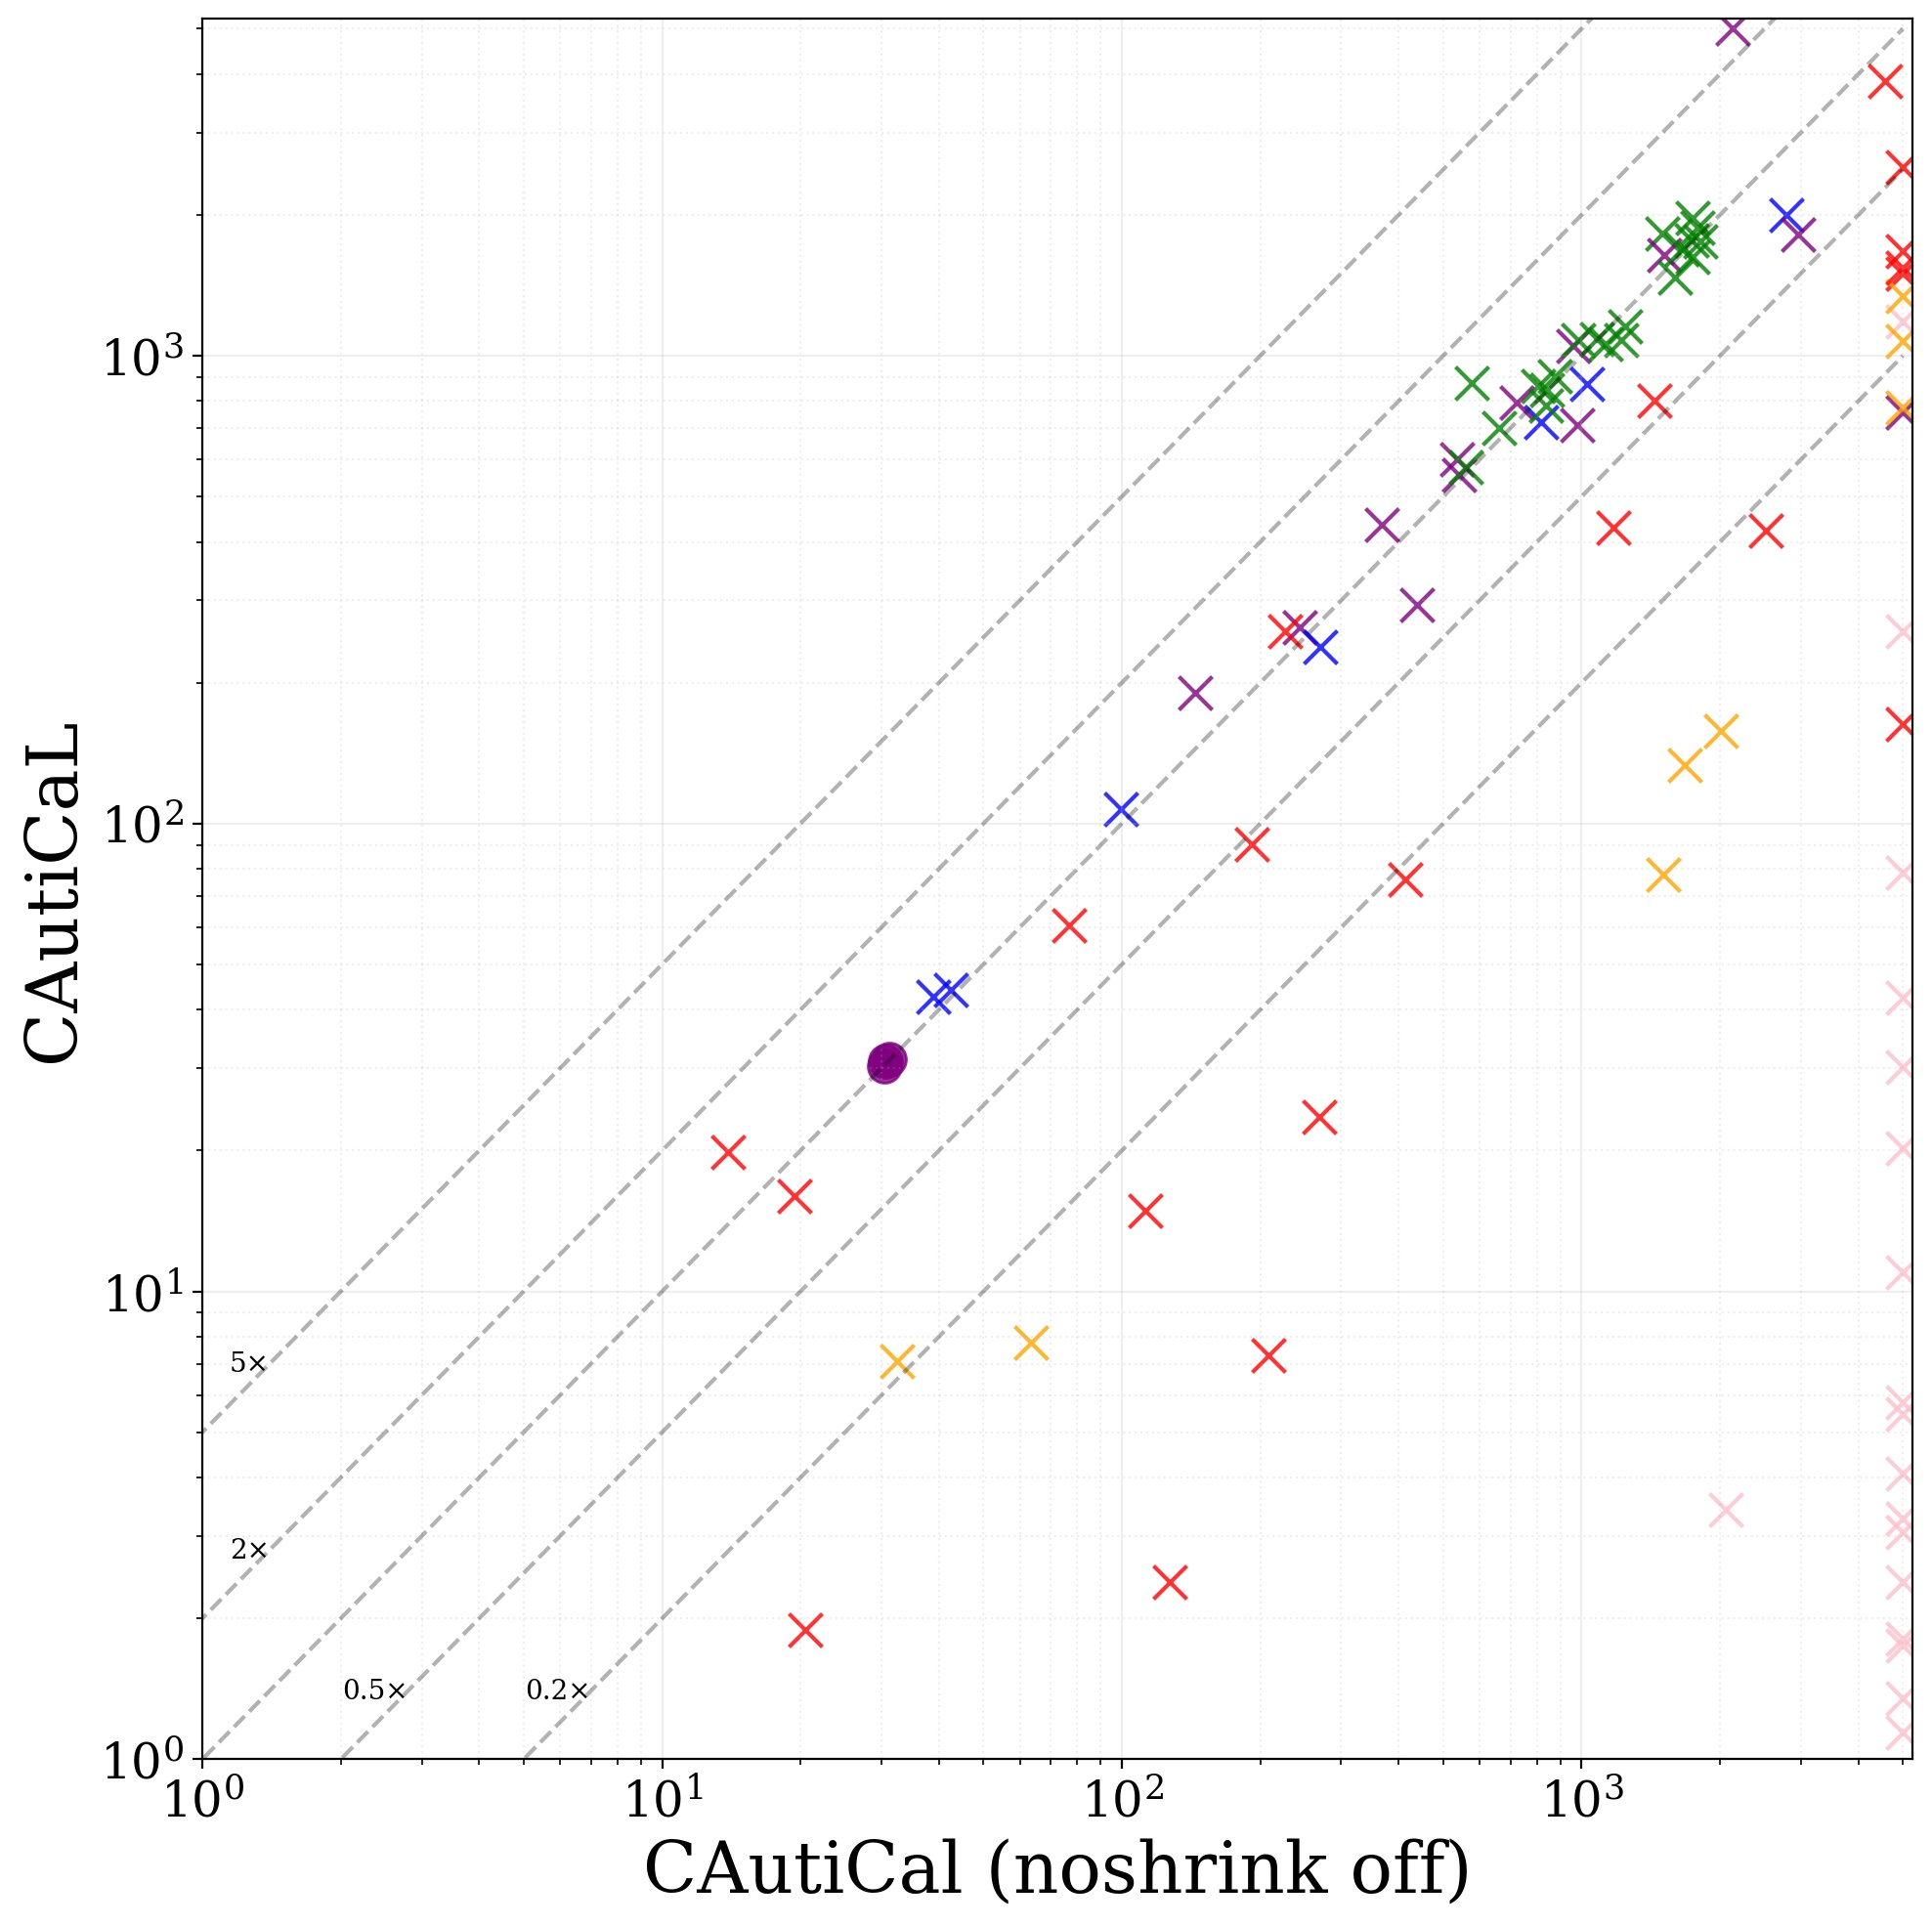
\includegraphics[width=\textwidth]{figs/globalnoshrink_heuristic_comparison.jpg}
    \caption{\tool compared to \tool with \textsf{shrink} turned off}
    \label{fig:global-no-shrink}
\end{subfigure}
\hfill
\begin{subfigure}[t]{0.3\textwidth}
    \centering
    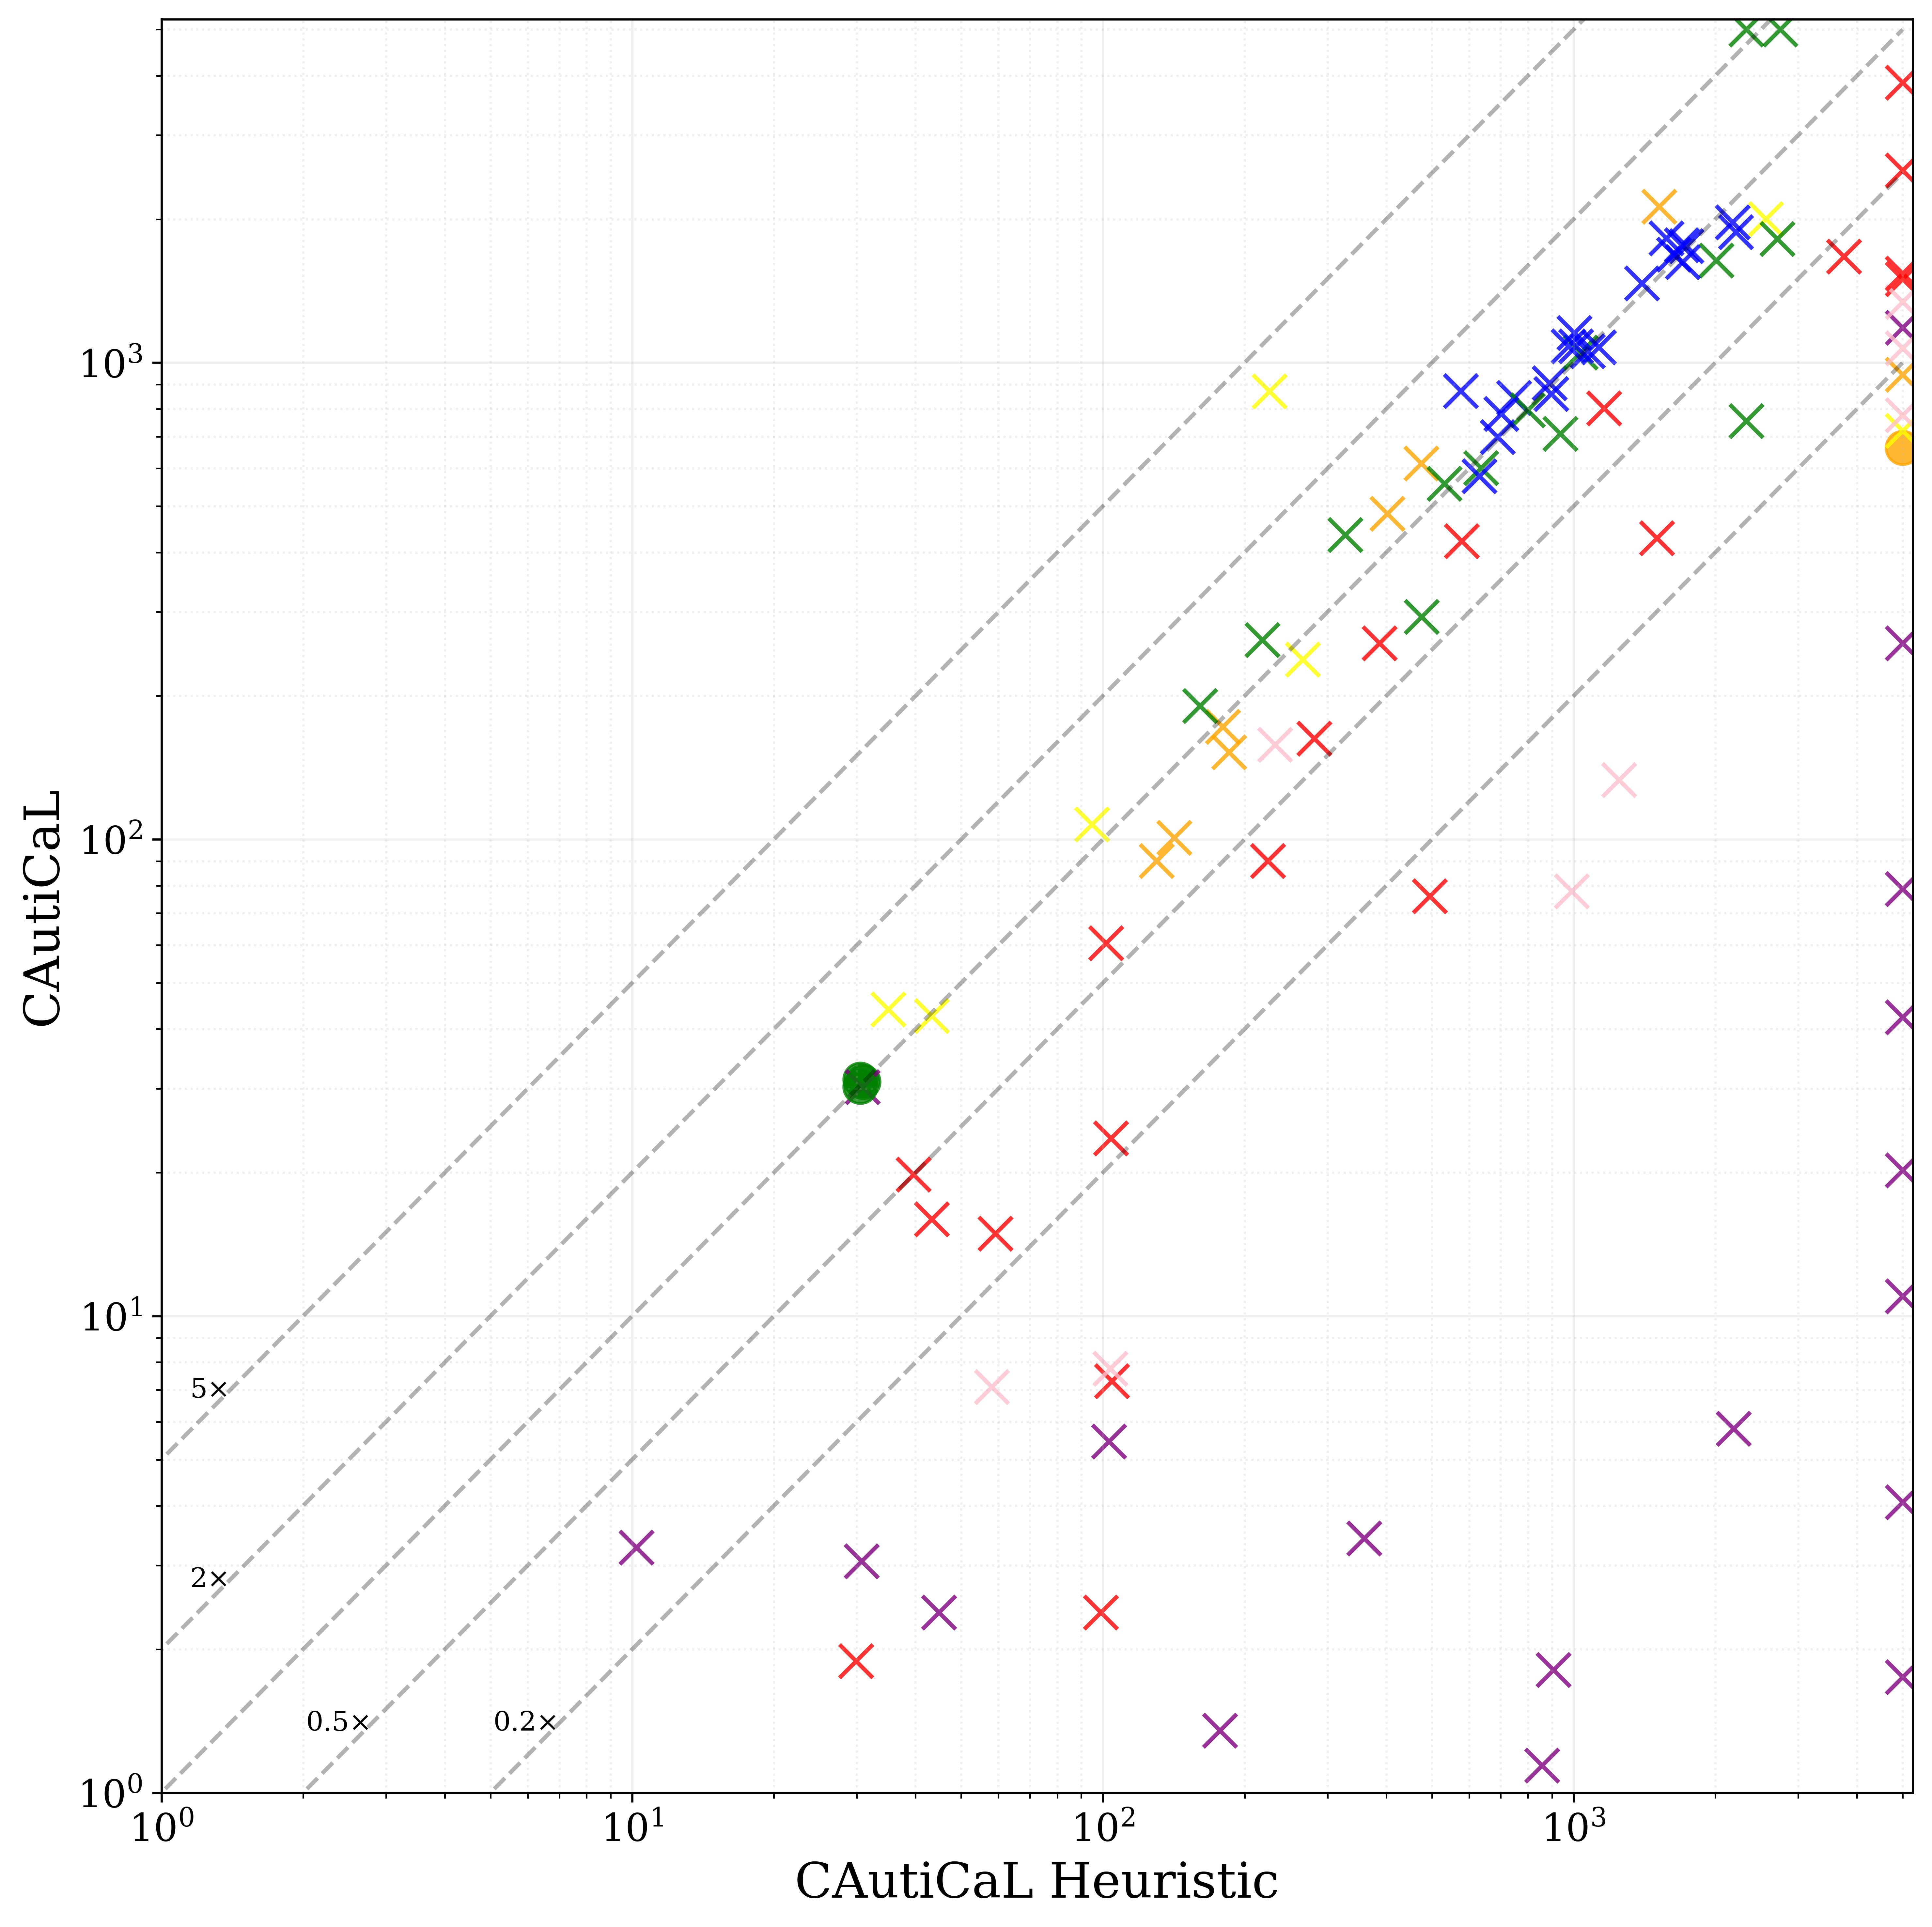
\includegraphics[width=\textwidth]{figs/globaldontfilter_heuristic_comparison.jpg}
    \caption{\tool compared to \tool with \textsf{filter-triv} turned off}
    \label{fig:globaldontfilter}
\end{subfigure}
\hfill
\begin{subfigure}[t]{0.3\textwidth}
    \centering
    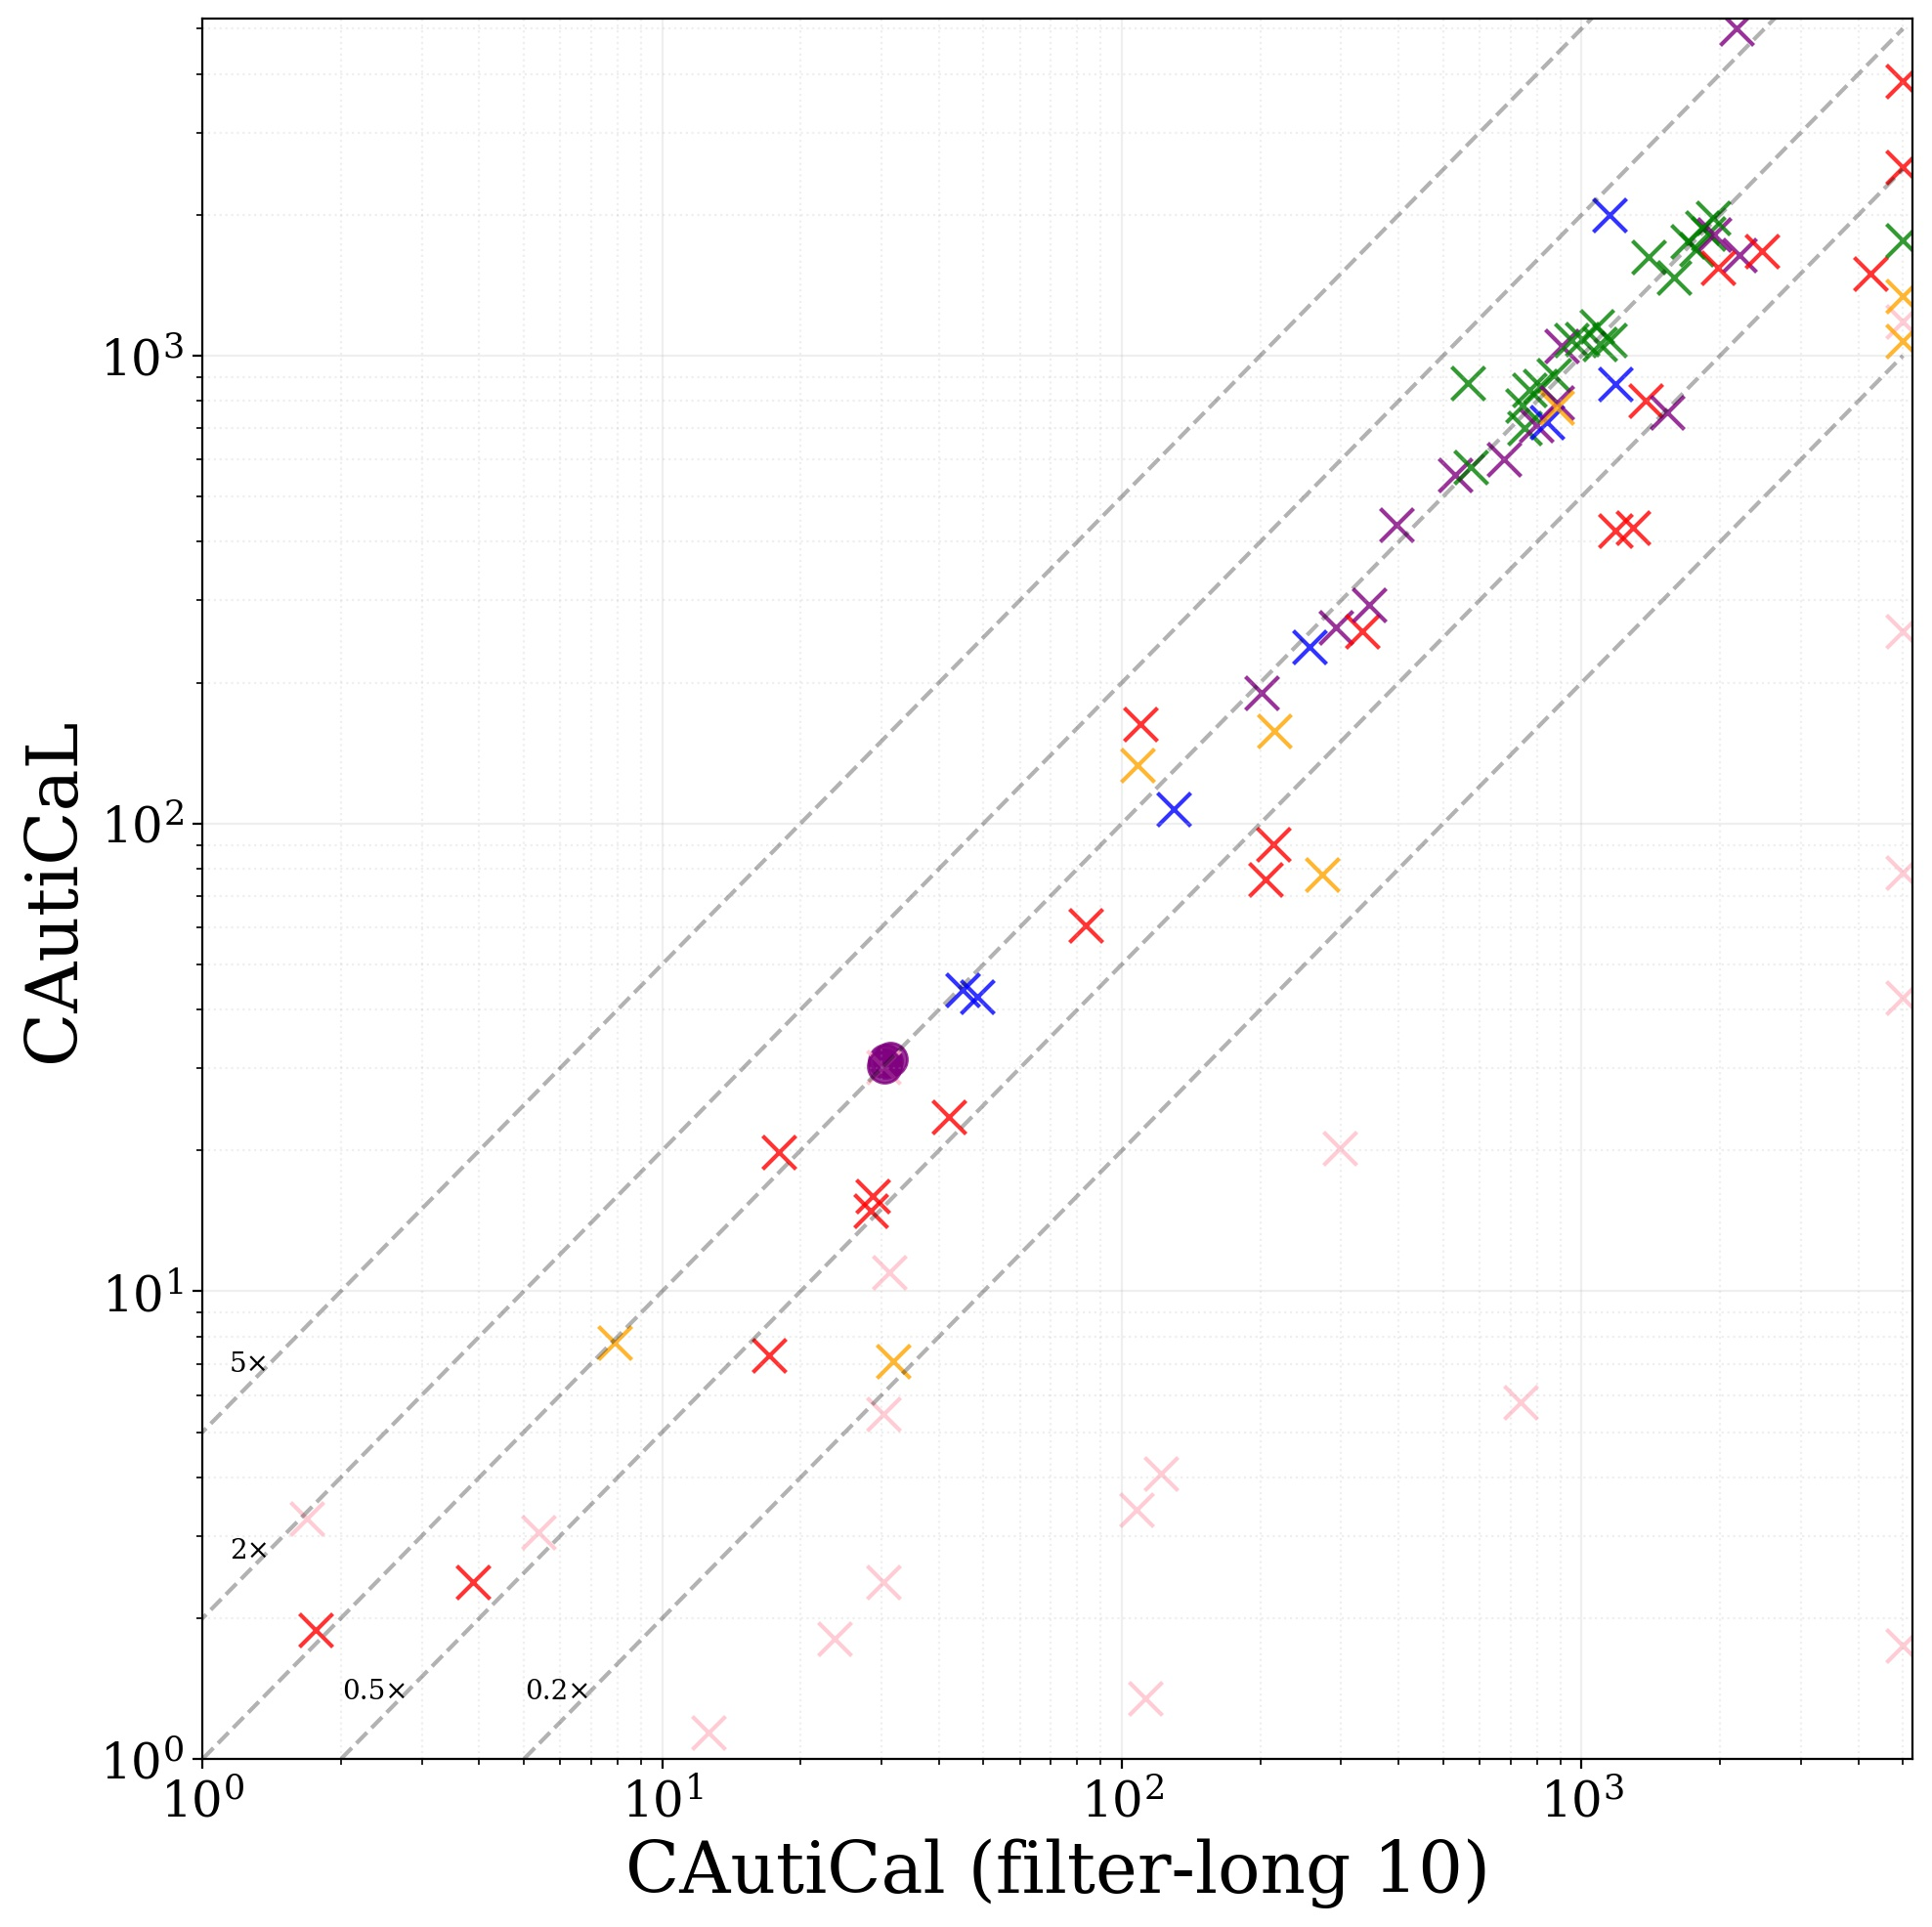
\includegraphics[width=\textwidth]{figs/globalmaxlen_heuristic_comparison.jpg}
    \caption{\tool compared to \tool with \textsf{filter-long} set to $10$}
    \label{fig:global-max-length}
\end{subfigure} 
\hfill
\begin{subfigure}[t]{0.3\textwidth}
    \centering
    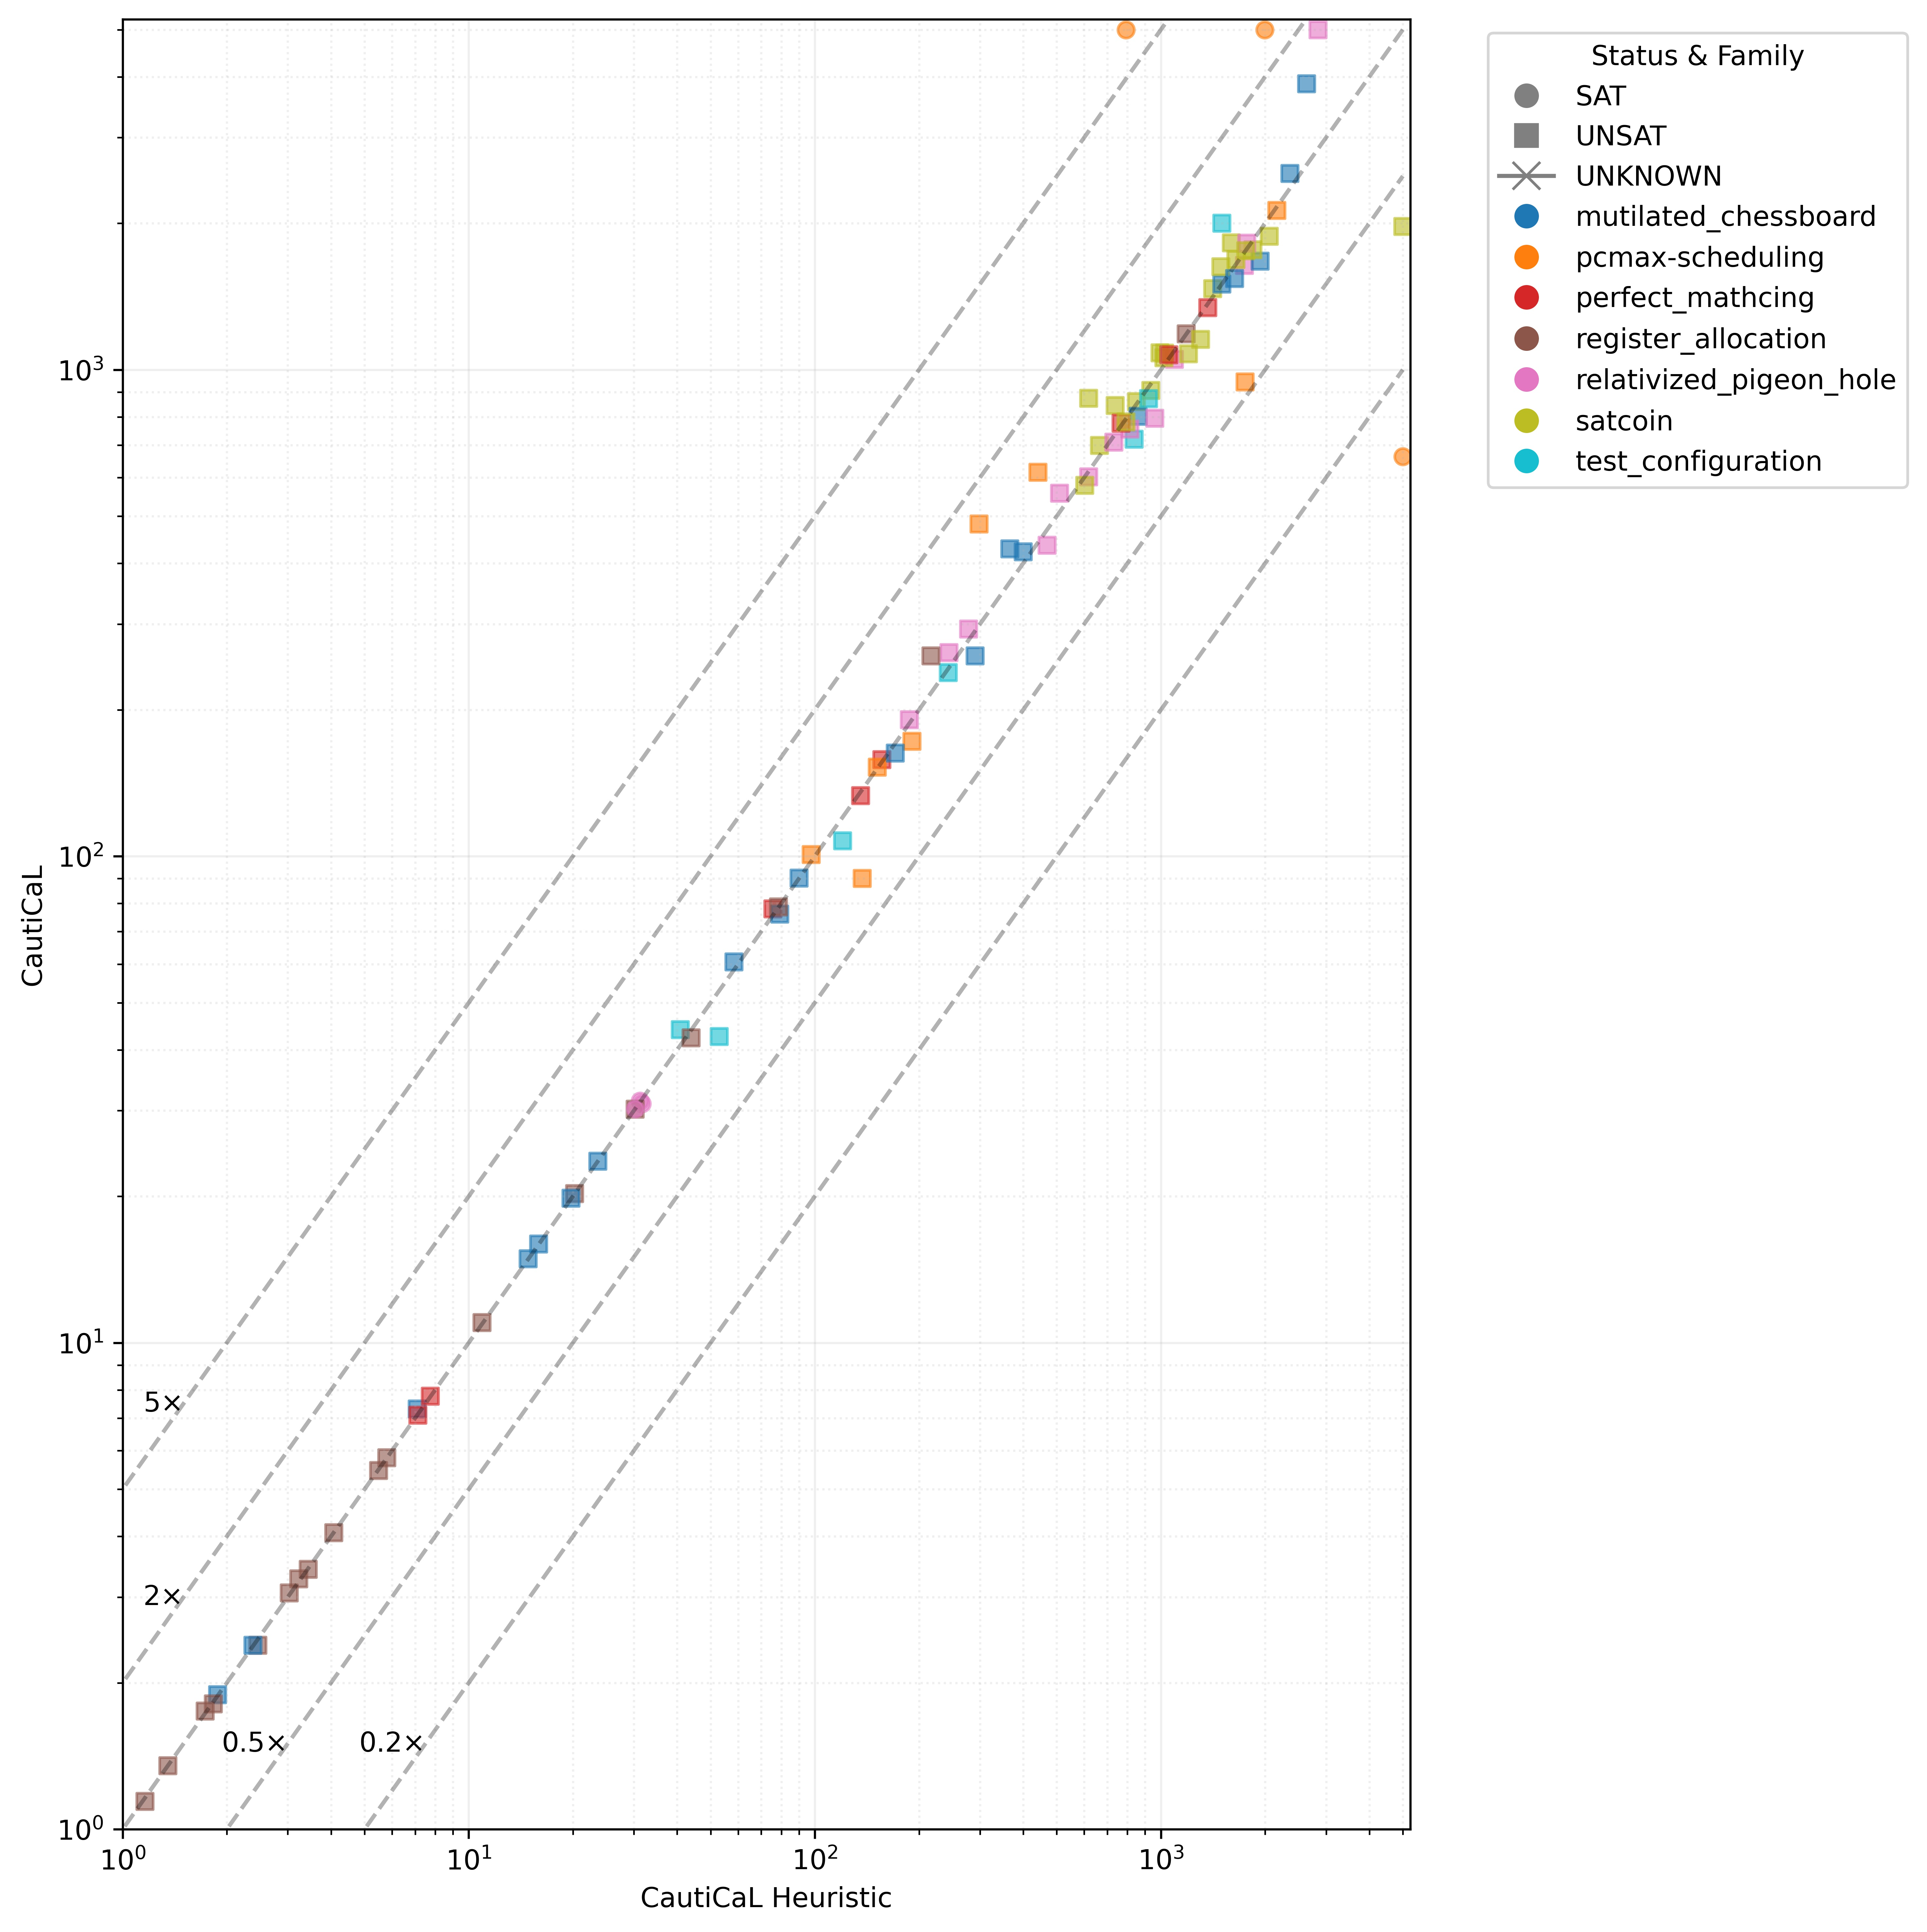
\includegraphics[width=\textwidth]{figs/global_time_lim_heuristic_comparison.jpg}
    \caption{\tool compared to \tool with \textsf{longer-preprocess} set to $100$ seconds}
    \label{fig:global-time-limit}
\end{subfigure}
\hfill    
\begin{subfigure}[t]{0.3\textwidth}
    \centering
    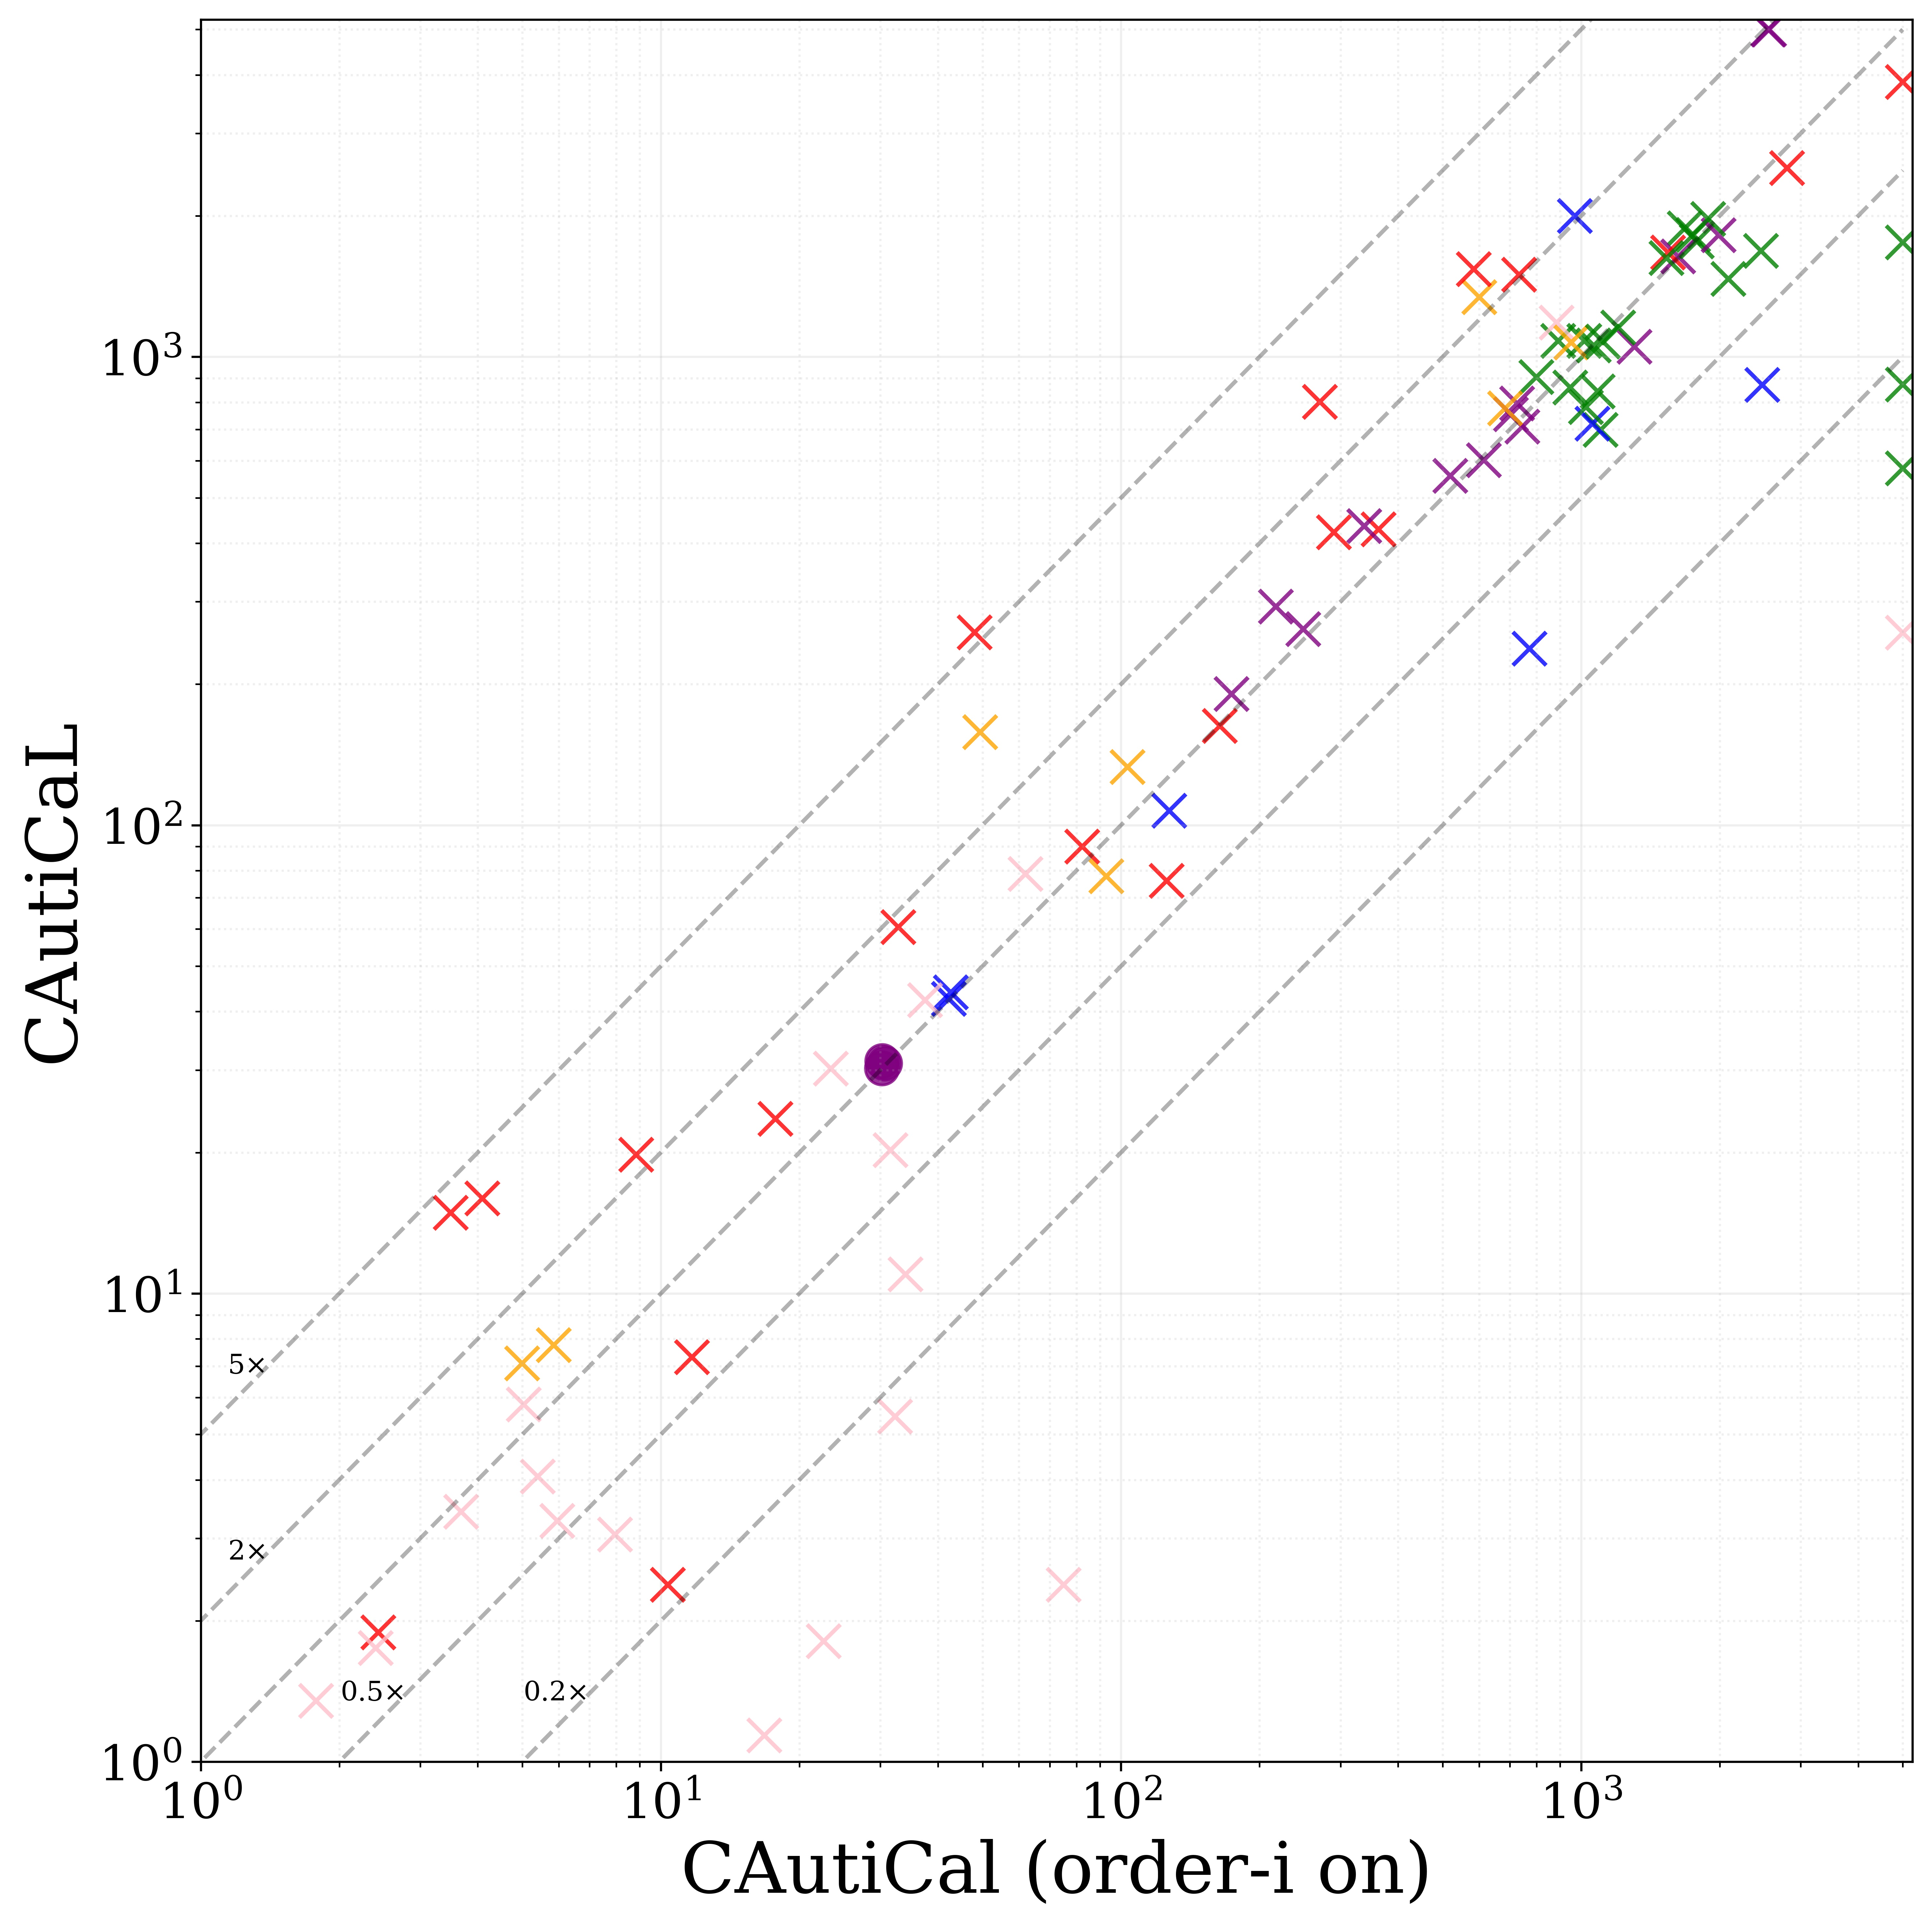
\includegraphics[width=\textwidth]{figs/globalisort_heuristic_comparison.jpg}
    \caption{\tool compared to \tool with \textsf{order-i} turned on}
    \label{fig:global-sort-i}
\end{subfigure}
\hfill
\begin{subfigure}[t]{0.3\textwidth}
    \centering
    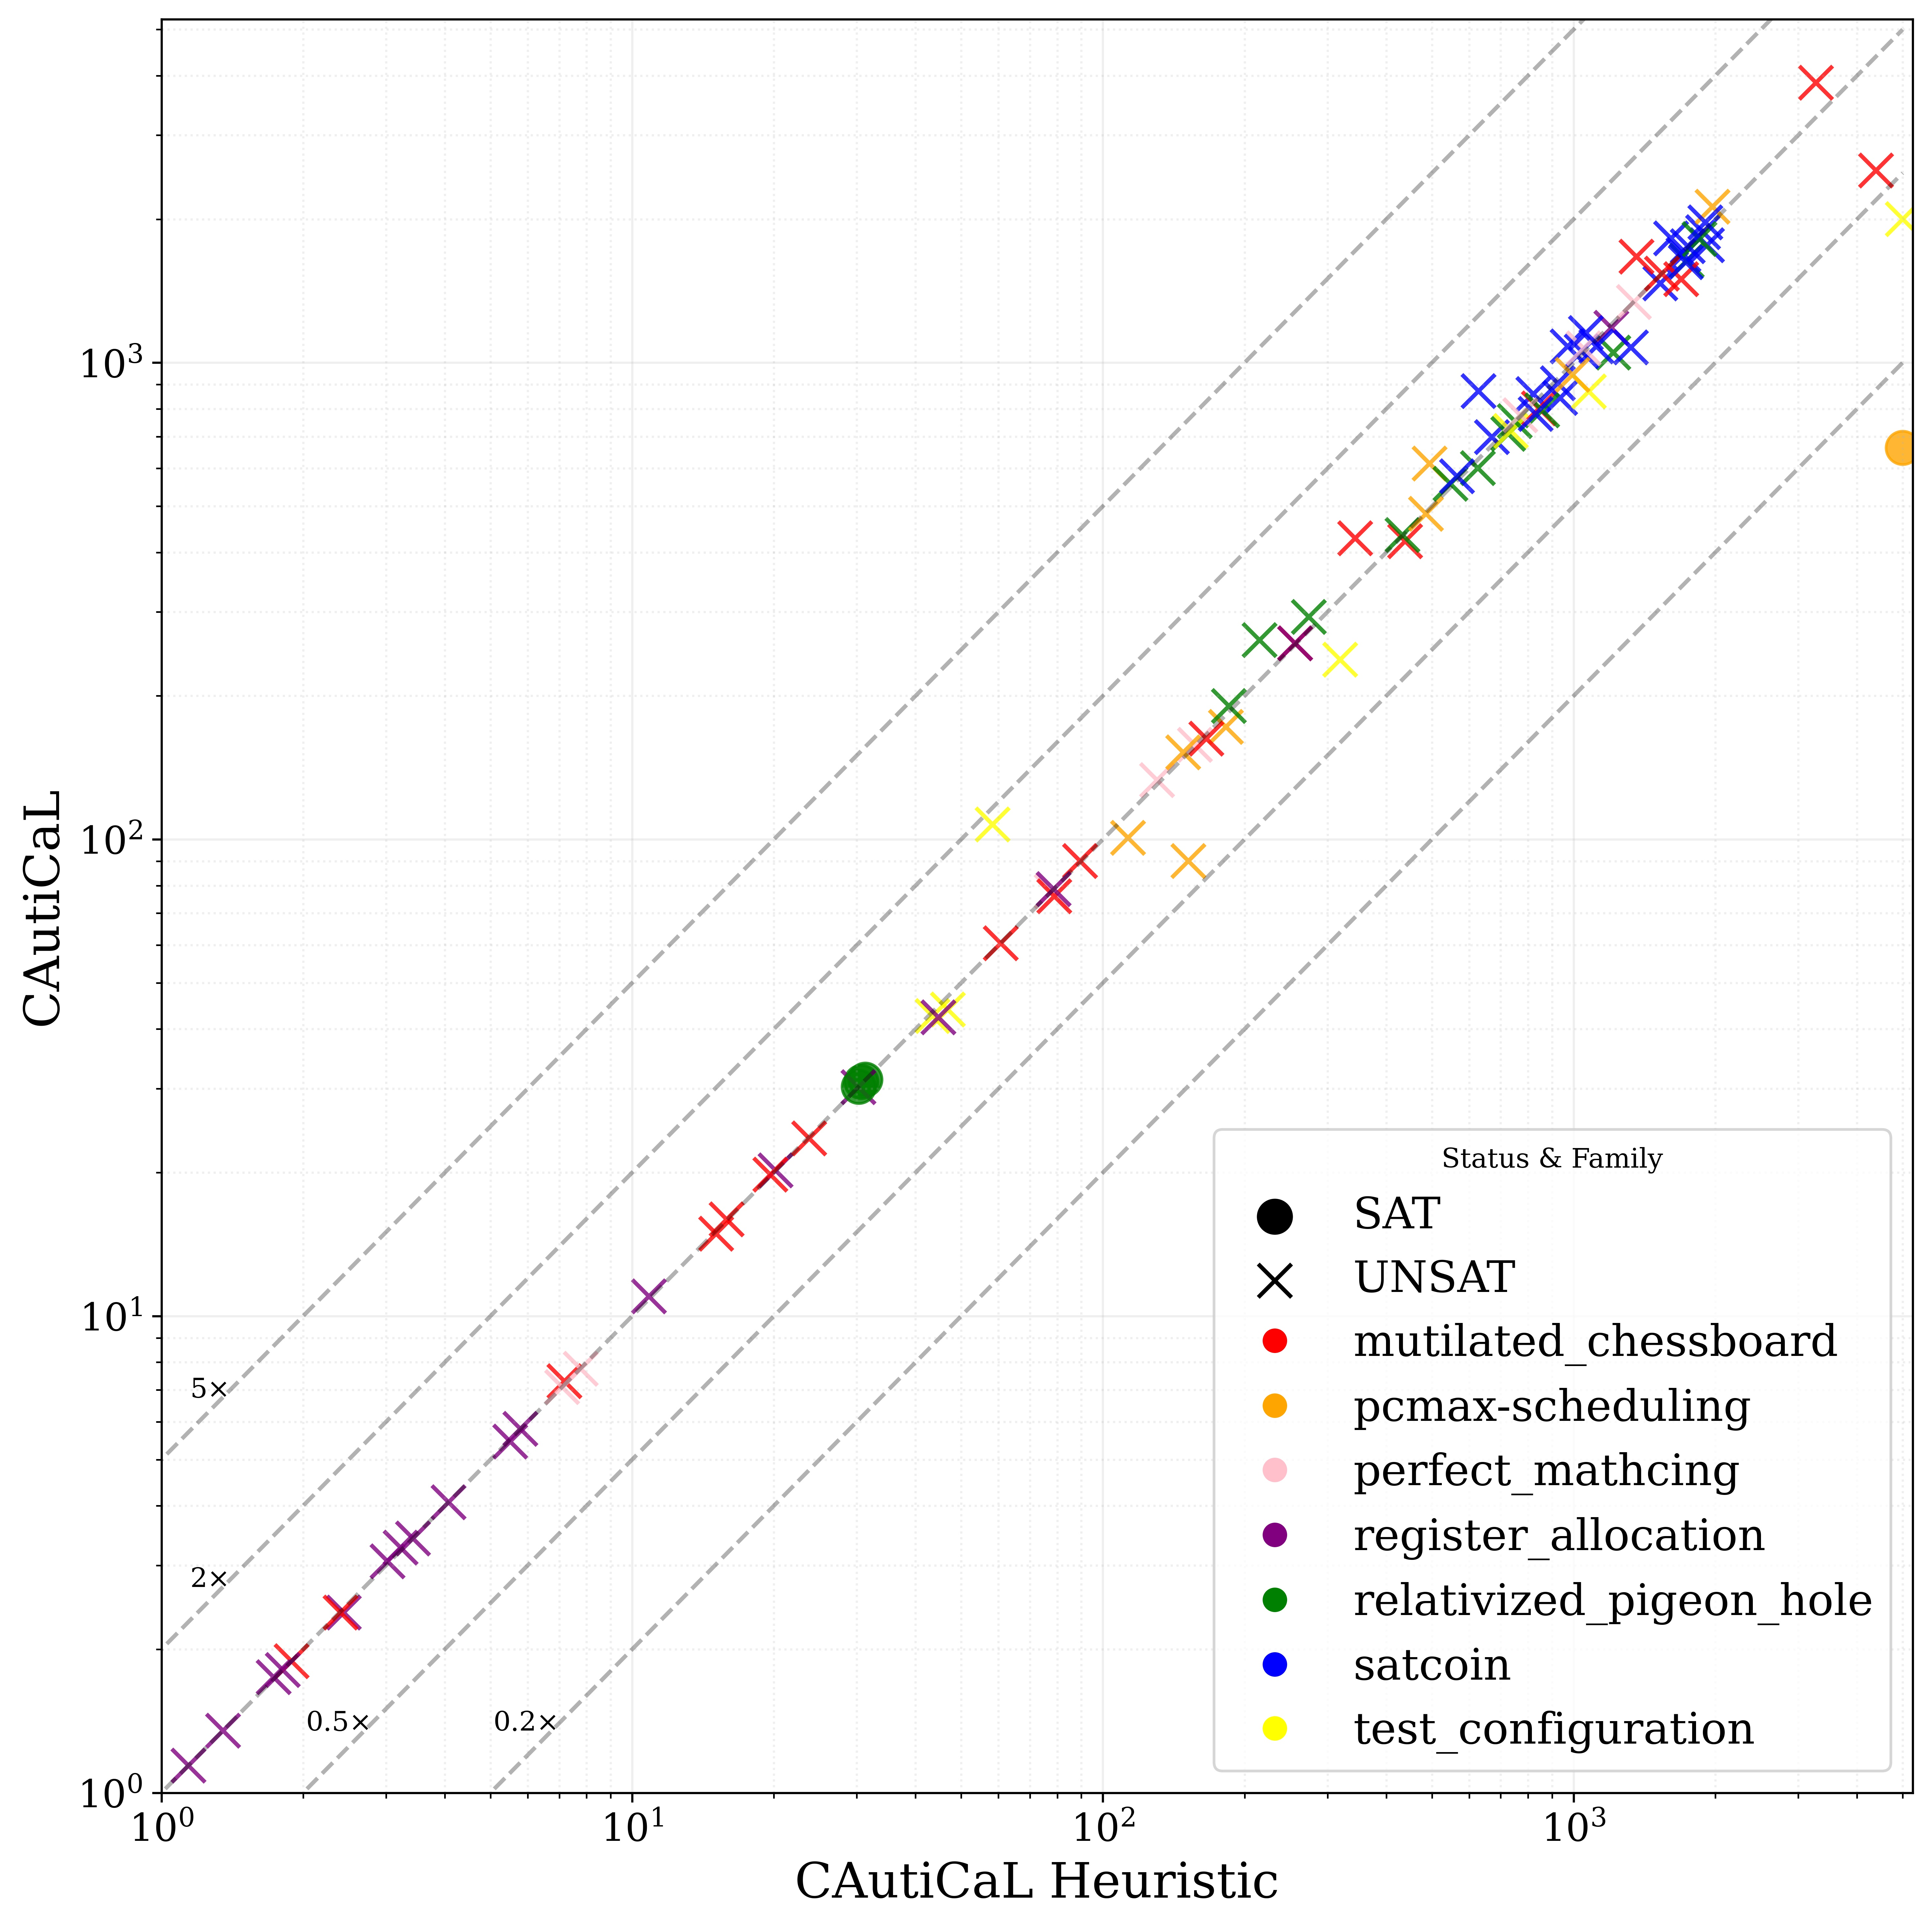
\includegraphics[width=\textwidth]{figs/globaltouch_heuristic_comparison.jpg}
    \caption{\tool compared to \tool with \textsf{select-j} turned on}
    \label{fig:global-touched}
\end{subfigure}
    \caption{Performance comparison of \tool with various heuristics turned on and off}~\label{fig:global-heuristics}
\end{figure*}

We compare the performance of \tool with \cadical and \prelearn on the
benchmarks from the '22, '23, and '24 SAT competition's main
tracks~\cite{satcomp2022,satcomp2023,satcomp2024}. We remove duplicates and
exclude all benchmarks with more than twenty million clauses as these are out of
scope for our technique. This gives us a total of 1,089 benchmarks. We exclude
\sadical from our evaluation as it only solves 22 of these benchmarks.

\autoref{tab:solver-stats} shows the number of instances solved by each solver.
Out of the total number solved, it shows the number of formulas for which
\prelearn and \tool learn additional \pr clauses, improve upon \cadical by at
least 5\%, and solve a formula that \cadical does not solve. 

We divide the benchmarks based on number of clauses (0-10k or 10k-20M) and
status (SAT or UNSAT). The number of clauses is a good indicator of the type of
benchmark, with many hard combinatorial problems containing fewer than ten
thousand clauses.
%, and many industrial clauses containing large numbers of clauses. Whether a
% formula is SAT or UNSAT is a good indicator of how helpful \pr clauses are.
% SAT formulas are sensitive to search heuristics, so adding a \pr clause can
% have a significant (positive or negative) effect on performance regardless of
% whether the clause is actually useful.

\autoref{fig:solver-comparison} shows \tool and \cadical's performance relative
to \cadical.
%  We only include points where \tool (for
% \autoref{subfig:cautical-vs-cadical-satcomp}) and \prelearn (for
% \autoref{subfig:cautical-vs-prelearn-satcomp}) learn at least one \pr clause.
\autoref{subfig:cautical-vs-cadical-satcomp} shows that \tool learns a large
number of \pr clauses for formulas which it solves quickly and \cadical times
out on. \autoref{subfig:cautical-vs-prelearn-performance} shows that \prelearn
also solve a number of formulas that \tool cannot, but \tool typically performs
better on formulas where it learns many \pr clauses.

We find that \tool can show a performance improvement or degradation on formulas
where it does not learn any \pr clauses. This is because as \tool runs, it
updates internal data structures such as watched literals, clause occurrence
lists, and variable phases. 

For instance, during the initial phase of searching for PR clauses, the solver
will decide on a literal. Unit propagation of this literal may lead to a
conflict, and the solver can learn the unit clause without any autarky/PR
reasoning. Unit clauses are not stored or treated as learned clauses inside
\cadical, but instead the literal becomes “fixed,” i.e., the solver treats the
literal as always true. For instance, this happens on the three satcoin
benchmarks where \tool shows the most improvement (see
\autoref{fig:solver-comparison-familis}).


PAR-2 score is a standard metric used to evaluate the performance of solvers. It
is evaluated as the sum of the runtimes of solved instances and twice the
timeout of unsolved instances. On this dataset, \cadical has a PAR-2 score of
3522 seconds, \prelearn has a PAR-2 score of 3331 seconds, and \tool has a PAR-2
score of 3442 seconds. 

\autoref{fig:cdf} shows the distribution of benchmarks solved by each solver.
Both \prelearn and \tool lag behind \cadical during the 30 second preprocessing
stage, but eventually solve more benchmarks. In the end, \prelearn solving the most
formulas at 771, followed by \tool at 754, and \cadical at 749. 

%  I don't know if this actually makes sense
% \tool solves 36 formulas that \cadical does not solve, while
% \prelearn solves 30 that \cadical does not solve. \tool improves on 219 formulas
% from \cadical, while \prelearn improves on 146 formulas. 





\tool exercises more selective \pr clause learning techniques, only learning \pr
clauses for 139 formulas, while \prelearn learns \pr clauses for 431 formulas
(see \autoref{fig:clauses-histogram}). On those formulas, \tool improves the
\cadical's runtime on 29.9\% of benchmarks, while \prelearn improves it on
24.7\% of benchmarks.








% prelearn PAR score:  3331.406813590451 cautical PAR score:  3442.137998163452
% cadical PAR score:  3521.7908356290172










% \subsection{\toolminus}

% Motivated by the fact that \tool improves mostly on formulas where it learns
% many clauses, we define a new variant \toolminus. After running the 30 second
% preprocessing step, if \toolminus does not learn at least $50$ \pr clauses, it
% will completely reset the context and run cadical. In
% \autoref{fig:toolminus-comparison}, we compare \tool to \prelearn and
% \toolminus to \prelearn on the SAT competition benchmarks.


% \begin{figure*}[!t] \centering \begin{subfigure}[t]{0.45\textwidth} \centering
%     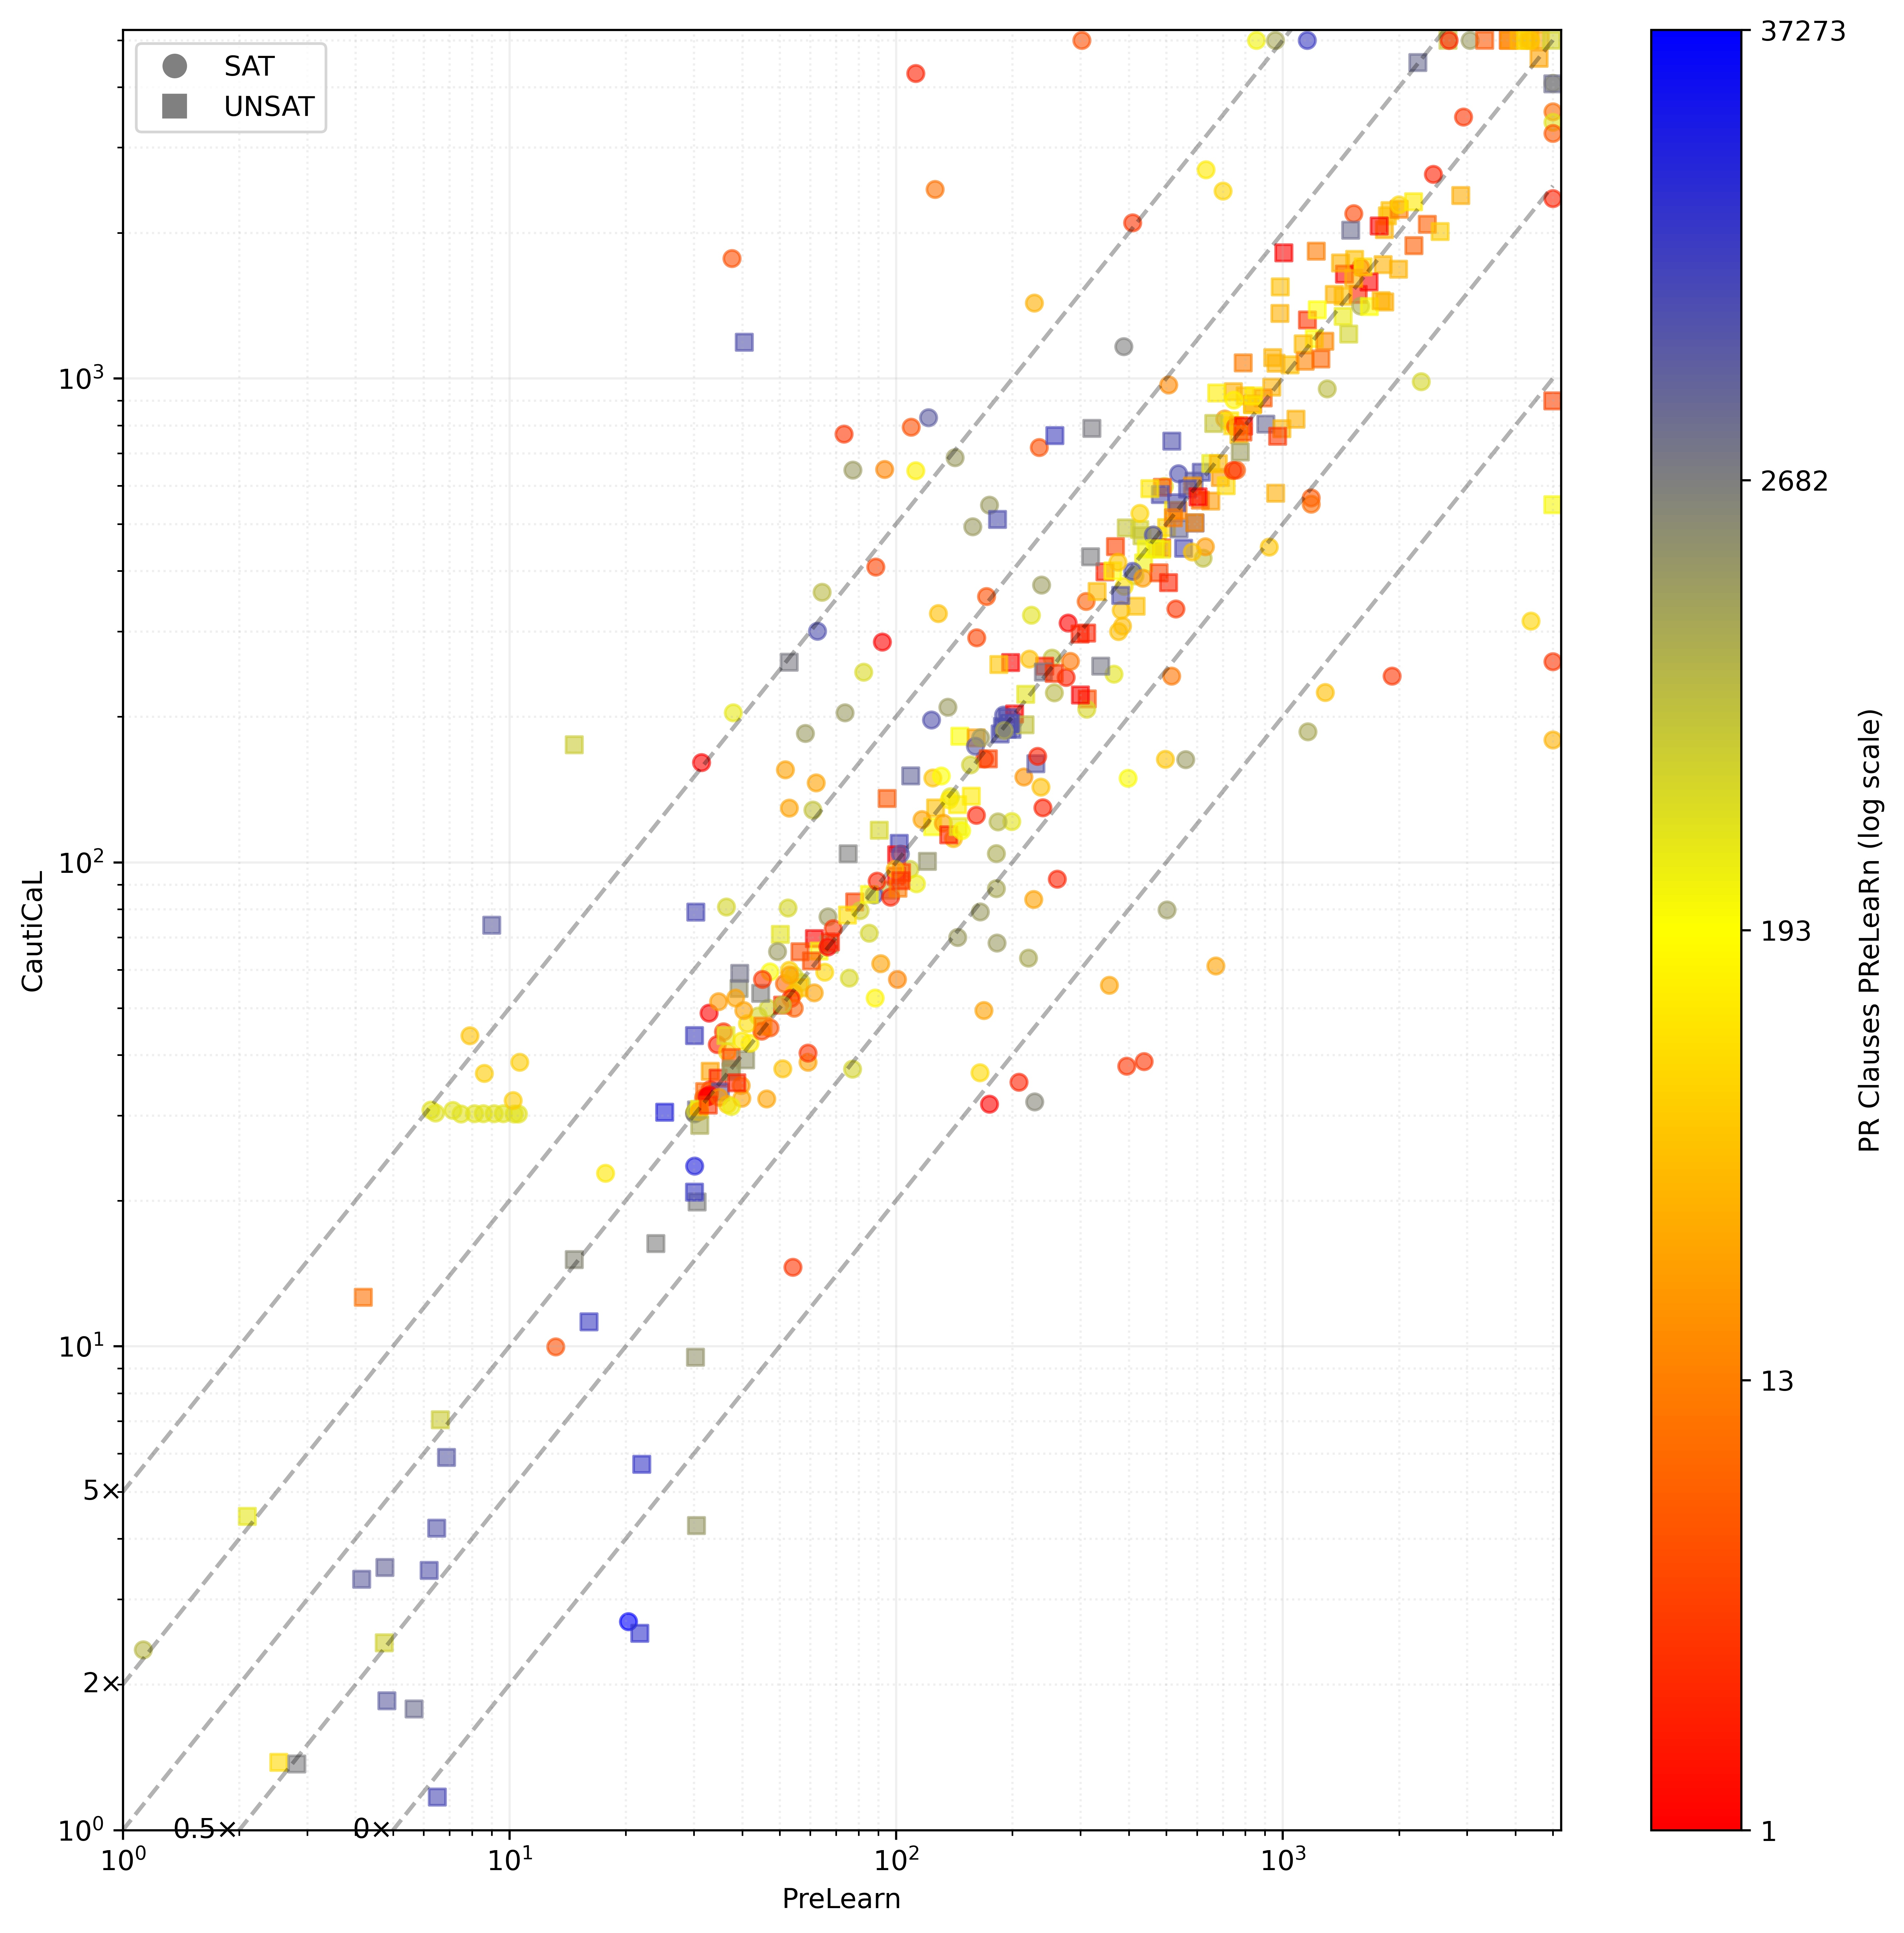
\includegraphics[width=\textwidth]{figs/prelearn_vs_cautical.jpg}
%     \caption{Comparing \tool to \prelearn. The color indicates the number of
%     \pr clauses learnt by \tool} \label{fig:cautical-vs-cadical}
%     \end{subfigure} % \hspace{0.06\textwidth}
%     \begin{subfigure}[t]{0.45\textwidth} \centering
%     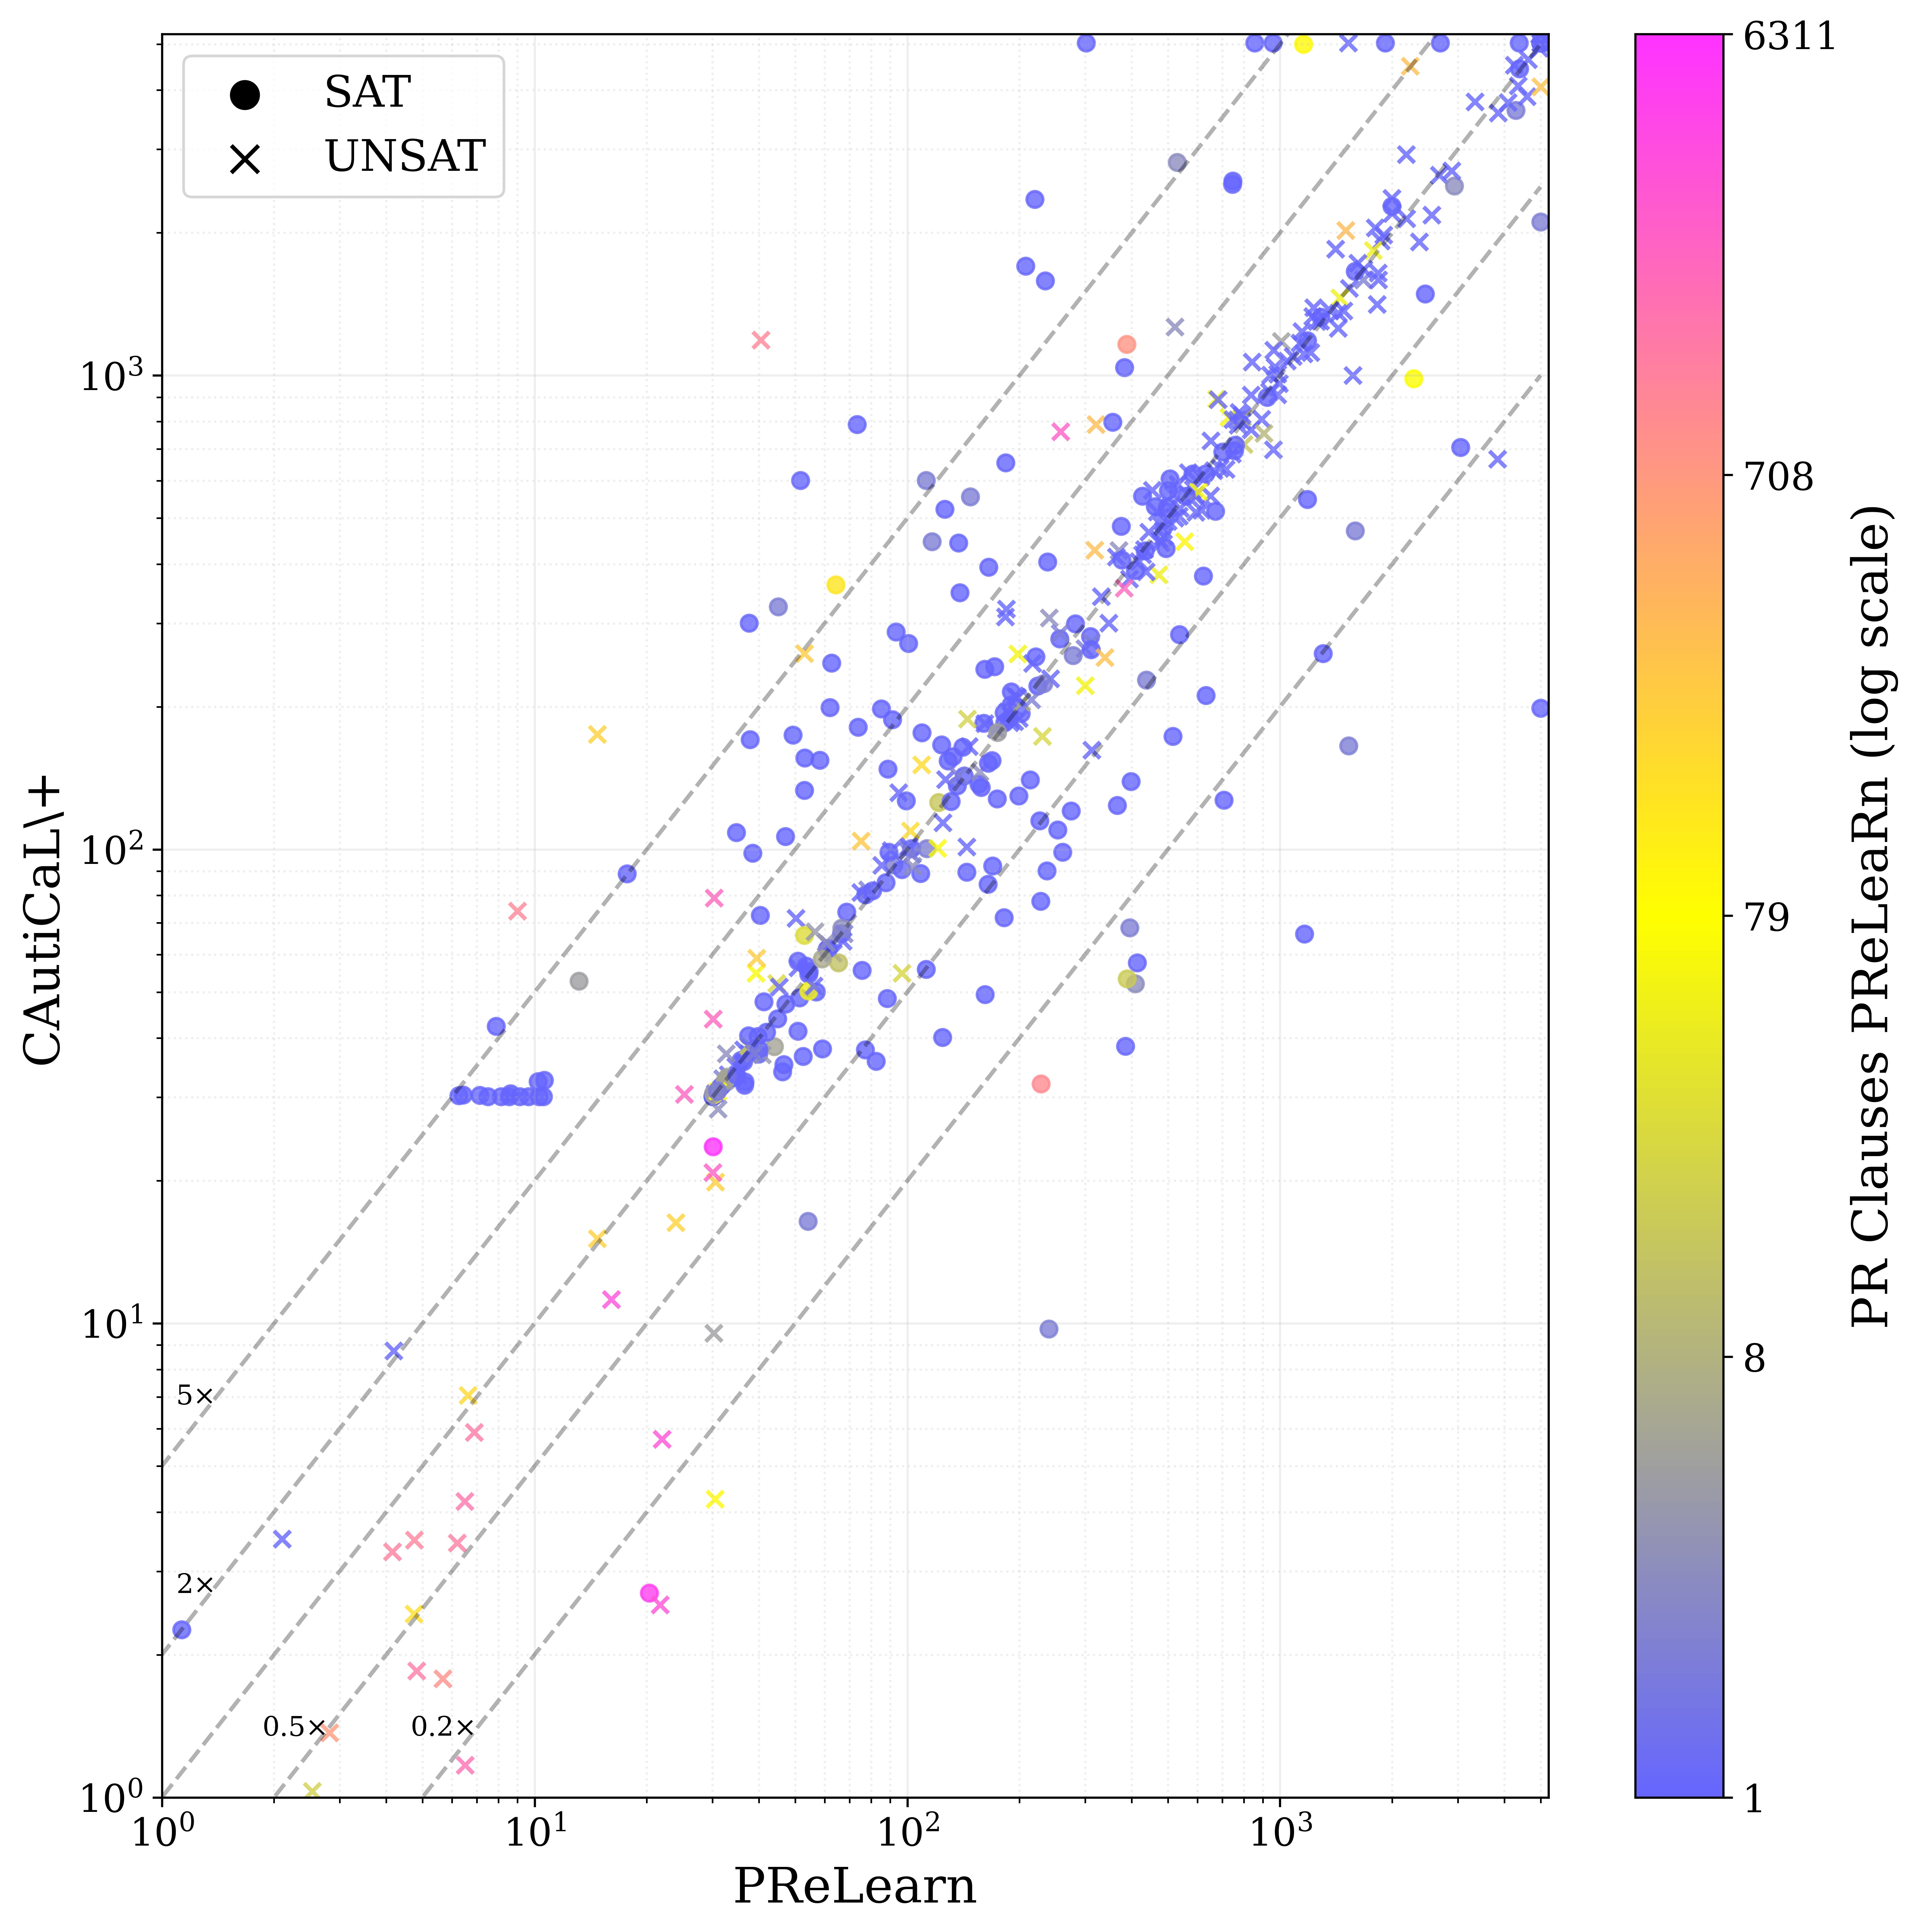
\includegraphics[width=\textwidth]{figs/prelearn_vs_cautical_minus_time.jpg}
%     \caption{Comparing \toolminus to \prelearn. The color indicates the number
%     of \pr clauses learnt by \toolminus} \label{fig:cautical-vs-prelearn}
%     \end{subfigure} \caption{Performance comparison of \tool with and
%     \toolminus with \prelearn on SAT competition benchmarks. We filter out all
%     benchmarks where both \tool and \prelearn do not learn any \pr clauses.
%     The color indicates the number of \pr clauses learnt by the \tool or
%     \toolminus.} % \label{fig:solver-comparison} \end{figure*}

% version of the graphs without filtering out clauses: prelearn_vs_cautical.jpg




\subsection{Discussion of Benchmark Families}~\label{subsec:eval-discussion}

We identify six benchmark families for which \pr clauses perform well. We choose
them based on prior work~\cite{prelearn} and our experiments on SAT competition
benchmarks:

\begin{enumerate}
    \item \texttt{mutilated-chessboard}: famous problem asking if one can use
    $2$-by-$1$ tiles to cover an $2n$-by-$2n$ chessboard with opposite corners
    removed. This is difficult for
    resolution~\cite{mutilatedchessboard-exponential}, but there exists $O(n^3)$
    \pr proofs~\cite{mutilatedchessboard-pr}.
    \item \texttt{perfect\_matching}: generalization of the pigeonhole principle
    and mutilated chessboard problems with various at-most-one
    constraints~\cite{bipartgen}.
    % \item \texttt{pcmax\_scheduling}: A problem encoding the scheduling
    % problem mapping $n$ tasks with known execution times to $m$ identical
    % processors~\cite{pcmax}. \item
    % https://helda.helsinki.fi/server/api/core/bitstreams/3f1f286b-3def-49e9-98ba-f887b1bc250e/content
    % -> page 31
    \item \texttt{register\_allocation}: the graph coloring problem generated by
    simulating register allocation on individual Python
    functions~\cite{register-allocation}.
    \item \texttt{relativized\_pigeonhole}: generalization of the pigeonhole
    principle where we place $n+1$ pigeons in $n$ holes with $k$ nesting places.
    % todo: ask joseph about citation
    \item \texttt{satcoin}: variant of a bitcoin mining problem~\cite{satcoin}.
    \item \texttt{test\_configuration}: is there a list of configurations of
    size $k$ that covers every pairwise combination of configurations of a SAT
    solver~\cite{test-configuration}.
\end{enumerate}

\begin{table}[h]
    \centering
    \begin{tabular}{lll}
        \hline
        Benchmark Family & Number of Clauses  & \tool \# \pr  \\
        \hline
        mutilated-chessboard & 900-3K & 115-351 \\
        perfect\_matching & 300-1K & 183-447 \\
        % pcmax\_scheduling & Task scheduling & Processor allocation \\
        register\_allocation & 1K-23K & 671-3322 \\
        relativized\_pigeonhole & 3K-2M & 469-9091 \\
        satcoin & 600K-600K & 0-0 \\
        test\_configuration & 31K-64K & 0-0 \\
        \hline
    \end{tabular}
    \caption{Overview of benchmark families used in evaluation}
    \label{tab:benchmark-families}
\end{table}

% These formulas are mostly UNSAT as these are most benefitted by \pr clause
% learning. SAT formulas are very sensitive to search heuristics, so adding a
% \pr clause can have a significant (positive or negative) effect on
% performance, regardless if a clause is actually useful.
\autoref{fig:solver-comparison-familis} compares the performance of \tool with
\cadical and \prelearn on these benchmark families. We do not evaluate \sadical
as it does very poorly on SAT competition benchmarks.
\autoref{tab:benchmark-families} provides a brief overview of the families: the
number of clauses in the original formulas (up to 1 significant digit) and the
number of \pr clauses learnt by \tool.

\tool compares favorably to \cadical on all benchmark families, showing especially large speedups on
\texttt{register\_allocation}, \texttt{mutilated\_chessboard} and
\texttt{perfect\_matching}. 
% \texttt{relativized\_pigeonhole}
% These are three of the formulas where \tool learns the most \pr clauses.
% Relativized pigeonhole is known to be somewhat difficult for \pr learning, but
% does have polynomial sized proofs for resolution~\cite{pr}.

\prelearn exhibits large speedups over \tool on \texttt{test\_configuration} and
\texttt{perfect\_matching}. \tool performs better on smaller instances of
\texttt{register\_allocation} and \texttt{mutilated\_chessboard}, while
\prelearn performs better on larger instances. \tool can also solve instances of
\texttt{satcoin} that \prelearn cannot.
%  Interestingly, \tool does not learn any \pr clauses for \texttt{satcoin}.







% \subsection{Analysis of heuristics}~\label{subsec:eval-heuristics}



%  shows that the time limit heuristic is not useful for \tool.
%  \autoref{fig:global-sort-i} shows that sorting $i$ beforehand by frequency
%  used is not useful. \autoref{fig:global-touched} shows that the touched
%  heuristic is not useful.






% \subsection{Research Questions}~\label{subsec:eval-research-questions}





\subsection{Heuristics}~\label{sec:heuristics}

\autoref{fig:global-heuristics} shows the performance of \tool with different
heuristics (discussed in \autoref{sec:implementation}) turned on and off. We
evaluate on the different benchmark families discussed in
\autoref{subsec:eval-discussion}.

First we consider turning three optimizations off.
\autoref{fig:global-no-shrink} compares \tool to \tool with
\textsf{shrink} turned off, i.e. we do not learn \pr clauses.
\autoref{fig:globaldontfilter} compares \tool to \tool with
\textsf{filter-triv} off, i.e. we do not filter trivial clauses.
\autoref{fig:global-max-length} compares \tool to \tool with
\textsf{filter-long} set to $10$, i.e. we filter out clauses of size $> 10$ (as
opposed to $2$ by default).

When we disable any of three optimizations, the performance is significantly
worse, especially on \texttt{perfect-matching}, \texttt{mutilated-chessboard},
and \texttt{register-allocation} benchmarks.

Next, we consider turning three potential ``optimizations'' on.
\autoref{fig:global-time-limit} sets \textsf{longer-preprocess} to 100 seconds
(as opposed to 30 seconds by default). \autoref{fig:global-sort-i} turns on
\textsf{order-i}, propagating the first literal $i$ ordered by which literals
occurs most frequently in the original formula. Finally,
\autoref{fig:global-heuristics} turns on \textsf{select-j}, picking $j$ the
second literal by whether it ``touches'' the first literal $i$.

Enabling any of these three ``optimizations'' does not improve performance and
in the case of \textsf{order-i}, it slightly hurts performance.

\subsection{Research Questions}~\label{subsec:researchquestions}

To conclude, we discuss the two research questions. 

For RQ1, \tool decisively outperforms all solvers except \sadical on the
pigeonhole benchmarks. On SAT competition benchmarks, \tool improves \cadical's
PAR-2 score by 2.2\%. \prelearn performs even better, improving \cadical's PAR-2
score by 5.4\%. However, compared to \prelearn, \tool outperforms \cadical on a
greater number of benchmarks (219 vs 146) and solves more benchmarks that
\cadical cannot solve (36 vs 30).

 
For RQ2, \tool is the only solver to solve all pigeonhole formulas after
scranfilization. Indeed, scranfilization has a negligible effect on \tool's
performance.

We experienced some success with robustness on the SAT competition benchmarks,
but not as significant as for pigeonhole. For instance, in the initial stage
when propagating first on literal $i$ (see \autoref{alg:methodology}), we
randomly pick the order for literal $i$.

Prior \pr learning approaches such as \prelearn used specific orderings of
literals to their advantage. We evaluated such an ordering in
\autoref{fig:global-sort-i} and found that it did not make a difference for
\tool.

